% AUTO-GENERATED by writeup/make_rehaul_close_accuracy.py -- do not edit; re-run the script.
% fig:rh_calibration: decile calibration of the elastic net and LightGBM, HAR benchmark and full predictor set.
\ifdefined\rhcaNdaysSpan\else% AUTO-GENERATED by writeup/make_rehaul_close_accuracy.py -- do not edit; re-run the script.
% \rhca... macros: closing-half-hour accuracy on both spans (tab:rh_close_accuracy) and the calibration
% diagnostics of the 12 pooled forecasts (tab:rh_calibration, fig:rh_calibration). Names: <Stat><Model><Set>
% <Sample><Span>; Model Ridge Lasso Enet Lgbm Xgb Rf Ols (pooled), Ci<Model> (trained on the closing half
% hour), Bm (closing-interval HAR benchmark); Set Har Full; Sample Close (16:00 bar) Bar (every bar);
% Span Span (2014-2024) Pre (2014-2019) Oos (T_oos, 2020-2024).
% --- spans and constants
\providecommand{\rhcaNdaysSpan}{}\renewcommand{\rhcaNdaysSpan}{2{,}579}  % trading days, 2014-01-02 .. 2024-04-30
\providecommand{\rhcaStartSpan}{}\renewcommand{\rhcaStartSpan}{2 January 2014}  % first day
\providecommand{\rhcaEndSpan}{}\renewcommand{\rhcaEndSpan}{30 April 2024}  % last day
\providecommand{\rhcaYearsSpan}{}\renewcommand{\rhcaYearsSpan}{2014--2024}  % years
\providecommand{\rhcaDMLagSpan}{}\renewcommand{\rhcaDMLagSpan}{8}  % Newey-West lag of the daily DM tests (dm_test automatic)
\providecommand{\rhcaHacLagBarSpan}{}\renewcommand{\rhcaHacLagBarSpan}{104}  % Newey-West lag of the every-bar MZ regressions, bars
\providecommand{\rhcaNdaysPre}{}\renewcommand{\rhcaNdaysPre}{1{,}496}  % trading days, 2014-01-02 .. 2019-12-31
\providecommand{\rhcaStartPre}{}\renewcommand{\rhcaStartPre}{2 January 2014}  % first day
\providecommand{\rhcaEndPre}{}\renewcommand{\rhcaEndPre}{31 December 2019}  % last day
\providecommand{\rhcaYearsPre}{}\renewcommand{\rhcaYearsPre}{2014--2019}  % years
\providecommand{\rhcaDMLagPre}{}\renewcommand{\rhcaDMLagPre}{7}  % Newey-West lag of the daily DM tests (dm_test automatic)
\providecommand{\rhcaHacLagBarPre}{}\renewcommand{\rhcaHacLagBarPre}{91}  % Newey-West lag of the every-bar MZ regressions, bars
\providecommand{\rhcaNdaysOos}{}\renewcommand{\rhcaNdaysOos}{1{,}082}  % trading days, 2020-01-03 .. 2024-04-30
\providecommand{\rhcaStartOos}{}\renewcommand{\rhcaStartOos}{3 January 2020}  % first day
\providecommand{\rhcaEndOos}{}\renewcommand{\rhcaEndOos}{30 April 2024}  % last day
\providecommand{\rhcaYearsOos}{}\renewcommand{\rhcaYearsOos}{2020--2024}  % years
\providecommand{\rhcaDMLagOos}{}\renewcommand{\rhcaDMLagOos}{6}  % Newey-West lag of the daily DM tests (dm_test automatic)
\providecommand{\rhcaHacLagBarOos}{}\renewcommand{\rhcaHacLagBarOos}{78}  % Newey-West lag of the every-bar MZ regressions, bars
\providecommand{\rhcaNbars}{}\renewcommand{\rhcaNbars}{33{,}527}  % scored bars of Table 1, 2014-2024
\providecommand{\rhcaCloseFirst}{}\renewcommand{\rhcaCloseFirst}{14 June 2006}  % first forecast of the closing-interval models
\providecommand{\rhcaMseExp}{}\renewcommand{\rhcaMseExp}{10}  % MSE printed x 10^this
\providecommand{\rhcaUnitExp}{}\renewcommand{\rhcaUnitExp}{6}  % MAE and the levels intercept printed x 10^this
\providecommand{\rhcaCrashStart}{}\renewcommand{\rhcaCrashStart}{24 February 2020}  % first day of the excluded window (make_rehaul_results.CRASH)
\providecommand{\rhcaCrashEnd}{}\renewcommand{\rhcaCrashEnd}{30 April 2020}  % last day of the excluded window
\providecommand{\rhcaTopDays}{}\renewcommand{\rhcaTopDays}{5}  % days in the extreme-day share
% --- closing half hour (16:00 bar): pooled forecasts, Span / Pre / Oos; Q QLIKE, Mse (x 10^10), Mae (x 10^6), Rsq R2_OOS %, Pct / Dm / P QLIKE full vs HAR, MsePct / MseDm / MseP, Gap / GapDm / GapP vs the closing-interval HAR benchmark (Oos only)
\providecommand{\rhcaQOlsHarCloseSpan}{}\renewcommand{\rhcaQOlsHarCloseSpan}{0.1269}
\providecommand{\rhcaMseOlsHarCloseSpan}{}\renewcommand{\rhcaMseOlsHarCloseSpan}{1.97}
\providecommand{\rhcaMaeOlsHarCloseSpan}{}\renewcommand{\rhcaMaeOlsHarCloseSpan}{2.92}
\providecommand{\rhcaRsqOlsHarCloseSpan}{}\renewcommand{\rhcaRsqOlsHarCloseSpan}{77.4}
\providecommand{\rhcaQRidgeHarCloseSpan}{}\renewcommand{\rhcaQRidgeHarCloseSpan}{0.1269}
\providecommand{\rhcaMseRidgeHarCloseSpan}{}\renewcommand{\rhcaMseRidgeHarCloseSpan}{1.97}
\providecommand{\rhcaMaeRidgeHarCloseSpan}{}\renewcommand{\rhcaMaeRidgeHarCloseSpan}{2.92}
\providecommand{\rhcaRsqRidgeHarCloseSpan}{}\renewcommand{\rhcaRsqRidgeHarCloseSpan}{77.4}
\providecommand{\rhcaQRidgeFullCloseSpan}{}\renewcommand{\rhcaQRidgeFullCloseSpan}{0.1291}
\providecommand{\rhcaMseRidgeFullCloseSpan}{}\renewcommand{\rhcaMseRidgeFullCloseSpan}{3.49}
\providecommand{\rhcaMaeRidgeFullCloseSpan}{}\renewcommand{\rhcaMaeRidgeFullCloseSpan}{3.22}
\providecommand{\rhcaRsqRidgeFullCloseSpan}{}\renewcommand{\rhcaRsqRidgeFullCloseSpan}{59.9}
\providecommand{\rhcaPctRidgeCloseSpan}{}\renewcommand{\rhcaPctRidgeCloseSpan}{1.8}  % QLIKE %, full vs HAR of the same class
\providecommand{\rhcaDmRidgeCloseSpan}{}\renewcommand{\rhcaDmRidgeCloseSpan}{0.67}
\providecommand{\rhcaPRidgeCloseSpan}{}\renewcommand{\rhcaPRidgeCloseSpan}{\ensuremath{p = 0.50}}
\providecommand{\rhcaMsePctRidgeCloseSpan}{}\renewcommand{\rhcaMsePctRidgeCloseSpan}{77.5}  % MSE %, full vs HAR
\providecommand{\rhcaMseDmRidgeCloseSpan}{}\renewcommand{\rhcaMseDmRidgeCloseSpan}{1.18}
\providecommand{\rhcaMsePRidgeCloseSpan}{}\renewcommand{\rhcaMsePRidgeCloseSpan}{\ensuremath{p = 0.24}}
\providecommand{\rhcaQLassoHarCloseSpan}{}\renewcommand{\rhcaQLassoHarCloseSpan}{0.1269}
\providecommand{\rhcaMseLassoHarCloseSpan}{}\renewcommand{\rhcaMseLassoHarCloseSpan}{1.97}
\providecommand{\rhcaMaeLassoHarCloseSpan}{}\renewcommand{\rhcaMaeLassoHarCloseSpan}{2.92}
\providecommand{\rhcaRsqLassoHarCloseSpan}{}\renewcommand{\rhcaRsqLassoHarCloseSpan}{77.4}
\providecommand{\rhcaQLassoFullCloseSpan}{}\renewcommand{\rhcaQLassoFullCloseSpan}{0.1322}
\providecommand{\rhcaMseLassoFullCloseSpan}{}\renewcommand{\rhcaMseLassoFullCloseSpan}{3.57}
\providecommand{\rhcaMaeLassoFullCloseSpan}{}\renewcommand{\rhcaMaeLassoFullCloseSpan}{3.24}
\providecommand{\rhcaRsqLassoFullCloseSpan}{}\renewcommand{\rhcaRsqLassoFullCloseSpan}{59.0}
\providecommand{\rhcaPctLassoCloseSpan}{}\renewcommand{\rhcaPctLassoCloseSpan}{4.2}  % QLIKE %, full vs HAR of the same class
\providecommand{\rhcaDmLassoCloseSpan}{}\renewcommand{\rhcaDmLassoCloseSpan}{1.35}
\providecommand{\rhcaPLassoCloseSpan}{}\renewcommand{\rhcaPLassoCloseSpan}{\ensuremath{p = 0.18}}
\providecommand{\rhcaMsePctLassoCloseSpan}{}\renewcommand{\rhcaMsePctLassoCloseSpan}{81.5}  % MSE %, full vs HAR
\providecommand{\rhcaMseDmLassoCloseSpan}{}\renewcommand{\rhcaMseDmLassoCloseSpan}{1.21}
\providecommand{\rhcaMsePLassoCloseSpan}{}\renewcommand{\rhcaMsePLassoCloseSpan}{\ensuremath{p = 0.23}}
\providecommand{\rhcaQEnetHarCloseSpan}{}\renewcommand{\rhcaQEnetHarCloseSpan}{0.1269}
\providecommand{\rhcaMseEnetHarCloseSpan}{}\renewcommand{\rhcaMseEnetHarCloseSpan}{1.97}
\providecommand{\rhcaMaeEnetHarCloseSpan}{}\renewcommand{\rhcaMaeEnetHarCloseSpan}{2.92}
\providecommand{\rhcaRsqEnetHarCloseSpan}{}\renewcommand{\rhcaRsqEnetHarCloseSpan}{77.4}
\providecommand{\rhcaQEnetFullCloseSpan}{}\renewcommand{\rhcaQEnetFullCloseSpan}{0.1276}
\providecommand{\rhcaMseEnetFullCloseSpan}{}\renewcommand{\rhcaMseEnetFullCloseSpan}{3.92}
\providecommand{\rhcaMaeEnetFullCloseSpan}{}\renewcommand{\rhcaMaeEnetFullCloseSpan}{3.28}
\providecommand{\rhcaRsqEnetFullCloseSpan}{}\renewcommand{\rhcaRsqEnetFullCloseSpan}{55.0}
\providecommand{\rhcaPctEnetCloseSpan}{}\renewcommand{\rhcaPctEnetCloseSpan}{0.6}  % QLIKE %, full vs HAR of the same class
\providecommand{\rhcaDmEnetCloseSpan}{}\renewcommand{\rhcaDmEnetCloseSpan}{0.24}
\providecommand{\rhcaPEnetCloseSpan}{}\renewcommand{\rhcaPEnetCloseSpan}{\ensuremath{p = 0.81}}
\providecommand{\rhcaMsePctEnetCloseSpan}{}\renewcommand{\rhcaMsePctEnetCloseSpan}{99.1}  % MSE %, full vs HAR
\providecommand{\rhcaMseDmEnetCloseSpan}{}\renewcommand{\rhcaMseDmEnetCloseSpan}{1.16}
\providecommand{\rhcaMsePEnetCloseSpan}{}\renewcommand{\rhcaMsePEnetCloseSpan}{\ensuremath{p = 0.25}}
\providecommand{\rhcaQLgbmHarCloseSpan}{}\renewcommand{\rhcaQLgbmHarCloseSpan}{0.1235}
\providecommand{\rhcaMseLgbmHarCloseSpan}{}\renewcommand{\rhcaMseLgbmHarCloseSpan}{1.77}
\providecommand{\rhcaMaeLgbmHarCloseSpan}{}\renewcommand{\rhcaMaeLgbmHarCloseSpan}{3.01}
\providecommand{\rhcaRsqLgbmHarCloseSpan}{}\renewcommand{\rhcaRsqLgbmHarCloseSpan}{79.6}
\providecommand{\rhcaQLgbmFullCloseSpan}{}\renewcommand{\rhcaQLgbmFullCloseSpan}{0.1202}
\providecommand{\rhcaMseLgbmFullCloseSpan}{}\renewcommand{\rhcaMseLgbmFullCloseSpan}{2.36}
\providecommand{\rhcaMaeLgbmFullCloseSpan}{}\renewcommand{\rhcaMaeLgbmFullCloseSpan}{3.02}
\providecommand{\rhcaRsqLgbmFullCloseSpan}{}\renewcommand{\rhcaRsqLgbmFullCloseSpan}{72.9}
\providecommand{\rhcaPctLgbmCloseSpan}{}\renewcommand{\rhcaPctLgbmCloseSpan}{\ensuremath{-}2.7}  % QLIKE %, full vs HAR of the same class
\providecommand{\rhcaDmLgbmCloseSpan}{}\renewcommand{\rhcaDmLgbmCloseSpan}{\ensuremath{-}1.76}
\providecommand{\rhcaPLgbmCloseSpan}{}\renewcommand{\rhcaPLgbmCloseSpan}{\ensuremath{p = 0.079}}
\providecommand{\rhcaMsePctLgbmCloseSpan}{}\renewcommand{\rhcaMsePctLgbmCloseSpan}{33.0}  % MSE %, full vs HAR
\providecommand{\rhcaMseDmLgbmCloseSpan}{}\renewcommand{\rhcaMseDmLgbmCloseSpan}{1.10}
\providecommand{\rhcaMsePLgbmCloseSpan}{}\renewcommand{\rhcaMsePLgbmCloseSpan}{\ensuremath{p = 0.27}}
\providecommand{\rhcaQXgbHarCloseSpan}{}\renewcommand{\rhcaQXgbHarCloseSpan}{0.1234}
\providecommand{\rhcaMseXgbHarCloseSpan}{}\renewcommand{\rhcaMseXgbHarCloseSpan}{1.73}
\providecommand{\rhcaMaeXgbHarCloseSpan}{}\renewcommand{\rhcaMaeXgbHarCloseSpan}{2.95}
\providecommand{\rhcaRsqXgbHarCloseSpan}{}\renewcommand{\rhcaRsqXgbHarCloseSpan}{80.1}
\providecommand{\rhcaQXgbFullCloseSpan}{}\renewcommand{\rhcaQXgbFullCloseSpan}{0.1195}
\providecommand{\rhcaMseXgbFullCloseSpan}{}\renewcommand{\rhcaMseXgbFullCloseSpan}{2.19}
\providecommand{\rhcaMaeXgbFullCloseSpan}{}\renewcommand{\rhcaMaeXgbFullCloseSpan}{3.01}
\providecommand{\rhcaRsqXgbFullCloseSpan}{}\renewcommand{\rhcaRsqXgbFullCloseSpan}{74.9}
\providecommand{\rhcaPctXgbCloseSpan}{}\renewcommand{\rhcaPctXgbCloseSpan}{\ensuremath{-}3.1}  % QLIKE %, full vs HAR of the same class
\providecommand{\rhcaDmXgbCloseSpan}{}\renewcommand{\rhcaDmXgbCloseSpan}{\ensuremath{-}2.01}
\providecommand{\rhcaPXgbCloseSpan}{}\renewcommand{\rhcaPXgbCloseSpan}{\ensuremath{p = 0.044}}
\providecommand{\rhcaMsePctXgbCloseSpan}{}\renewcommand{\rhcaMsePctXgbCloseSpan}{26.3}  % MSE %, full vs HAR
\providecommand{\rhcaMseDmXgbCloseSpan}{}\renewcommand{\rhcaMseDmXgbCloseSpan}{1.09}
\providecommand{\rhcaMsePXgbCloseSpan}{}\renewcommand{\rhcaMsePXgbCloseSpan}{\ensuremath{p = 0.28}}
\providecommand{\rhcaQRfHarCloseSpan}{}\renewcommand{\rhcaQRfHarCloseSpan}{0.1266}
\providecommand{\rhcaMseRfHarCloseSpan}{}\renewcommand{\rhcaMseRfHarCloseSpan}{1.63}
\providecommand{\rhcaMaeRfHarCloseSpan}{}\renewcommand{\rhcaMaeRfHarCloseSpan}{2.91}
\providecommand{\rhcaRsqRfHarCloseSpan}{}\renewcommand{\rhcaRsqRfHarCloseSpan}{81.3}
\providecommand{\rhcaQRfFullCloseSpan}{}\renewcommand{\rhcaQRfFullCloseSpan}{0.1246}
\providecommand{\rhcaMseRfFullCloseSpan}{}\renewcommand{\rhcaMseRfFullCloseSpan}{1.95}
\providecommand{\rhcaMaeRfFullCloseSpan}{}\renewcommand{\rhcaMaeRfFullCloseSpan}{2.97}
\providecommand{\rhcaRsqRfFullCloseSpan}{}\renewcommand{\rhcaRsqRfFullCloseSpan}{77.6}
\providecommand{\rhcaPctRfCloseSpan}{}\renewcommand{\rhcaPctRfCloseSpan}{\ensuremath{-}1.6}  % QLIKE %, full vs HAR of the same class
\providecommand{\rhcaDmRfCloseSpan}{}\renewcommand{\rhcaDmRfCloseSpan}{\ensuremath{-}1.03}
\providecommand{\rhcaPRfCloseSpan}{}\renewcommand{\rhcaPRfCloseSpan}{\ensuremath{p = 0.30}}
\providecommand{\rhcaMsePctRfCloseSpan}{}\renewcommand{\rhcaMsePctRfCloseSpan}{19.7}  % MSE %, full vs HAR
\providecommand{\rhcaMseDmRfCloseSpan}{}\renewcommand{\rhcaMseDmRfCloseSpan}{1.11}
\providecommand{\rhcaMsePRfCloseSpan}{}\renewcommand{\rhcaMsePRfCloseSpan}{\ensuremath{p = 0.27}}
\providecommand{\rhcaQOlsHarClosePre}{}\renewcommand{\rhcaQOlsHarClosePre}{0.1365}
\providecommand{\rhcaMseOlsHarClosePre}{}\renewcommand{\rhcaMseOlsHarClosePre}{0.32}
\providecommand{\rhcaMaeOlsHarClosePre}{}\renewcommand{\rhcaMaeOlsHarClosePre}{1.74}
\providecommand{\rhcaRsqOlsHarClosePre}{}\renewcommand{\rhcaRsqOlsHarClosePre}{73.9}
\providecommand{\rhcaQRidgeHarClosePre}{}\renewcommand{\rhcaQRidgeHarClosePre}{0.1365}
\providecommand{\rhcaMseRidgeHarClosePre}{}\renewcommand{\rhcaMseRidgeHarClosePre}{0.32}
\providecommand{\rhcaMaeRidgeHarClosePre}{}\renewcommand{\rhcaMaeRidgeHarClosePre}{1.74}
\providecommand{\rhcaRsqRidgeHarClosePre}{}\renewcommand{\rhcaRsqRidgeHarClosePre}{73.9}
\providecommand{\rhcaQRidgeFullClosePre}{}\renewcommand{\rhcaQRidgeFullClosePre}{0.1309}
\providecommand{\rhcaMseRidgeFullClosePre}{}\renewcommand{\rhcaMseRidgeFullClosePre}{0.28}
\providecommand{\rhcaMaeRidgeFullClosePre}{}\renewcommand{\rhcaMaeRidgeFullClosePre}{1.66}
\providecommand{\rhcaRsqRidgeFullClosePre}{}\renewcommand{\rhcaRsqRidgeFullClosePre}{77.3}
\providecommand{\rhcaPctRidgeClosePre}{}\renewcommand{\rhcaPctRidgeClosePre}{\ensuremath{-}4.1}  % QLIKE %, full vs HAR of the same class
\providecommand{\rhcaDmRidgeClosePre}{}\renewcommand{\rhcaDmRidgeClosePre}{\ensuremath{-}1.42}
\providecommand{\rhcaPRidgeClosePre}{}\renewcommand{\rhcaPRidgeClosePre}{\ensuremath{p = 0.16}}
\providecommand{\rhcaMsePctRidgeClosePre}{}\renewcommand{\rhcaMsePctRidgeClosePre}{\ensuremath{-}13.1}  % MSE %, full vs HAR
\providecommand{\rhcaMseDmRidgeClosePre}{}\renewcommand{\rhcaMseDmRidgeClosePre}{\ensuremath{-}1.79}
\providecommand{\rhcaMsePRidgeClosePre}{}\renewcommand{\rhcaMsePRidgeClosePre}{\ensuremath{p = 0.074}}
\providecommand{\rhcaQLassoHarClosePre}{}\renewcommand{\rhcaQLassoHarClosePre}{0.1365}
\providecommand{\rhcaMseLassoHarClosePre}{}\renewcommand{\rhcaMseLassoHarClosePre}{0.32}
\providecommand{\rhcaMaeLassoHarClosePre}{}\renewcommand{\rhcaMaeLassoHarClosePre}{1.74}
\providecommand{\rhcaRsqLassoHarClosePre}{}\renewcommand{\rhcaRsqLassoHarClosePre}{73.9}
\providecommand{\rhcaQLassoFullClosePre}{}\renewcommand{\rhcaQLassoFullClosePre}{0.1333}
\providecommand{\rhcaMseLassoFullClosePre}{}\renewcommand{\rhcaMseLassoFullClosePre}{0.27}
\providecommand{\rhcaMaeLassoFullClosePre}{}\renewcommand{\rhcaMaeLassoFullClosePre}{1.65}
\providecommand{\rhcaRsqLassoFullClosePre}{}\renewcommand{\rhcaRsqLassoFullClosePre}{78.0}
\providecommand{\rhcaPctLassoClosePre}{}\renewcommand{\rhcaPctLassoClosePre}{\ensuremath{-}2.3}  % QLIKE %, full vs HAR of the same class
\providecommand{\rhcaDmLassoClosePre}{}\renewcommand{\rhcaDmLassoClosePre}{\ensuremath{-}0.67}
\providecommand{\rhcaPLassoClosePre}{}\renewcommand{\rhcaPLassoClosePre}{\ensuremath{p = 0.50}}
\providecommand{\rhcaMsePctLassoClosePre}{}\renewcommand{\rhcaMsePctLassoClosePre}{\ensuremath{-}15.8}  % MSE %, full vs HAR
\providecommand{\rhcaMseDmLassoClosePre}{}\renewcommand{\rhcaMseDmLassoClosePre}{\ensuremath{-}1.78}
\providecommand{\rhcaMsePLassoClosePre}{}\renewcommand{\rhcaMsePLassoClosePre}{\ensuremath{p = 0.075}}
\providecommand{\rhcaQEnetHarClosePre}{}\renewcommand{\rhcaQEnetHarClosePre}{0.1365}
\providecommand{\rhcaMseEnetHarClosePre}{}\renewcommand{\rhcaMseEnetHarClosePre}{0.32}
\providecommand{\rhcaMaeEnetHarClosePre}{}\renewcommand{\rhcaMaeEnetHarClosePre}{1.74}
\providecommand{\rhcaRsqEnetHarClosePre}{}\renewcommand{\rhcaRsqEnetHarClosePre}{73.9}
\providecommand{\rhcaQEnetFullClosePre}{}\renewcommand{\rhcaQEnetFullClosePre}{0.1300}
\providecommand{\rhcaMseEnetFullClosePre}{}\renewcommand{\rhcaMseEnetFullClosePre}{0.28}
\providecommand{\rhcaMaeEnetFullClosePre}{}\renewcommand{\rhcaMaeEnetFullClosePre}{1.64}
\providecommand{\rhcaRsqEnetFullClosePre}{}\renewcommand{\rhcaRsqEnetFullClosePre}{77.6}
\providecommand{\rhcaPctEnetClosePre}{}\renewcommand{\rhcaPctEnetClosePre}{\ensuremath{-}4.8}  % QLIKE %, full vs HAR of the same class
\providecommand{\rhcaDmEnetClosePre}{}\renewcommand{\rhcaDmEnetClosePre}{\ensuremath{-}1.80}
\providecommand{\rhcaPEnetClosePre}{}\renewcommand{\rhcaPEnetClosePre}{\ensuremath{p = 0.071}}
\providecommand{\rhcaMsePctEnetClosePre}{}\renewcommand{\rhcaMsePctEnetClosePre}{\ensuremath{-}14.4}  % MSE %, full vs HAR
\providecommand{\rhcaMseDmEnetClosePre}{}\renewcommand{\rhcaMseDmEnetClosePre}{\ensuremath{-}1.90}
\providecommand{\rhcaMsePEnetClosePre}{}\renewcommand{\rhcaMsePEnetClosePre}{\ensuremath{p = 0.058}}
\providecommand{\rhcaQLgbmHarClosePre}{}\renewcommand{\rhcaQLgbmHarClosePre}{0.1333}
\providecommand{\rhcaMseLgbmHarClosePre}{}\renewcommand{\rhcaMseLgbmHarClosePre}{0.40}
\providecommand{\rhcaMaeLgbmHarClosePre}{}\renewcommand{\rhcaMaeLgbmHarClosePre}{1.84}
\providecommand{\rhcaRsqLgbmHarClosePre}{}\renewcommand{\rhcaRsqLgbmHarClosePre}{68.1}
\providecommand{\rhcaQLgbmFullClosePre}{}\renewcommand{\rhcaQLgbmFullClosePre}{0.1287}
\providecommand{\rhcaMseLgbmFullClosePre}{}\renewcommand{\rhcaMseLgbmFullClosePre}{0.37}
\providecommand{\rhcaMaeLgbmFullClosePre}{}\renewcommand{\rhcaMaeLgbmFullClosePre}{1.74}
\providecommand{\rhcaRsqLgbmFullClosePre}{}\renewcommand{\rhcaRsqLgbmFullClosePre}{70.5}
\providecommand{\rhcaPctLgbmClosePre}{}\renewcommand{\rhcaPctLgbmClosePre}{\ensuremath{-}3.4}  % QLIKE %, full vs HAR of the same class
\providecommand{\rhcaDmLgbmClosePre}{}\renewcommand{\rhcaDmLgbmClosePre}{\ensuremath{-}1.99}
\providecommand{\rhcaPLgbmClosePre}{}\renewcommand{\rhcaPLgbmClosePre}{\ensuremath{p = 0.046}}
\providecommand{\rhcaMsePctLgbmClosePre}{}\renewcommand{\rhcaMsePctLgbmClosePre}{\ensuremath{-}7.5}  % MSE %, full vs HAR
\providecommand{\rhcaMseDmLgbmClosePre}{}\renewcommand{\rhcaMseDmLgbmClosePre}{\ensuremath{-}1.78}
\providecommand{\rhcaMsePLgbmClosePre}{}\renewcommand{\rhcaMsePLgbmClosePre}{\ensuremath{p = 0.076}}
\providecommand{\rhcaQXgbHarClosePre}{}\renewcommand{\rhcaQXgbHarClosePre}{0.1331}
\providecommand{\rhcaMseXgbHarClosePre}{}\renewcommand{\rhcaMseXgbHarClosePre}{0.37}
\providecommand{\rhcaMaeXgbHarClosePre}{}\renewcommand{\rhcaMaeXgbHarClosePre}{1.82}
\providecommand{\rhcaRsqXgbHarClosePre}{}\renewcommand{\rhcaRsqXgbHarClosePre}{70.0}
\providecommand{\rhcaQXgbFullClosePre}{}\renewcommand{\rhcaQXgbFullClosePre}{0.1277}
\providecommand{\rhcaMseXgbFullClosePre}{}\renewcommand{\rhcaMseXgbFullClosePre}{0.33}
\providecommand{\rhcaMaeXgbFullClosePre}{}\renewcommand{\rhcaMaeXgbFullClosePre}{1.74}
\providecommand{\rhcaRsqXgbFullClosePre}{}\renewcommand{\rhcaRsqXgbFullClosePre}{73.0}
\providecommand{\rhcaPctXgbClosePre}{}\renewcommand{\rhcaPctXgbClosePre}{\ensuremath{-}4.0}  % QLIKE %, full vs HAR of the same class
\providecommand{\rhcaDmXgbClosePre}{}\renewcommand{\rhcaDmXgbClosePre}{\ensuremath{-}2.13}
\providecommand{\rhcaPXgbClosePre}{}\renewcommand{\rhcaPXgbClosePre}{\ensuremath{p = 0.033}}
\providecommand{\rhcaMsePctXgbClosePre}{}\renewcommand{\rhcaMsePctXgbClosePre}{\ensuremath{-}10.0}  % MSE %, full vs HAR
\providecommand{\rhcaMseDmXgbClosePre}{}\renewcommand{\rhcaMseDmXgbClosePre}{\ensuremath{-}1.66}
\providecommand{\rhcaMsePXgbClosePre}{}\renewcommand{\rhcaMsePXgbClosePre}{\ensuremath{p = 0.097}}
\providecommand{\rhcaQRfHarClosePre}{}\renewcommand{\rhcaQRfHarClosePre}{0.1364}
\providecommand{\rhcaMseRfHarClosePre}{}\renewcommand{\rhcaMseRfHarClosePre}{0.36}
\providecommand{\rhcaMaeRfHarClosePre}{}\renewcommand{\rhcaMaeRfHarClosePre}{1.81}
\providecommand{\rhcaRsqRfHarClosePre}{}\renewcommand{\rhcaRsqRfHarClosePre}{70.7}
\providecommand{\rhcaQRfFullClosePre}{}\renewcommand{\rhcaQRfFullClosePre}{0.1335}
\providecommand{\rhcaMseRfFullClosePre}{}\renewcommand{\rhcaMseRfFullClosePre}{0.34}
\providecommand{\rhcaMaeRfFullClosePre}{}\renewcommand{\rhcaMaeRfFullClosePre}{1.77}
\providecommand{\rhcaRsqRfFullClosePre}{}\renewcommand{\rhcaRsqRfFullClosePre}{72.3}
\providecommand{\rhcaPctRfClosePre}{}\renewcommand{\rhcaPctRfClosePre}{\ensuremath{-}2.1}  % QLIKE %, full vs HAR of the same class
\providecommand{\rhcaDmRfClosePre}{}\renewcommand{\rhcaDmRfClosePre}{\ensuremath{-}1.14}
\providecommand{\rhcaPRfClosePre}{}\renewcommand{\rhcaPRfClosePre}{\ensuremath{p = 0.25}}
\providecommand{\rhcaMsePctRfClosePre}{}\renewcommand{\rhcaMsePctRfClosePre}{\ensuremath{-}5.3}  % MSE %, full vs HAR
\providecommand{\rhcaMseDmRfClosePre}{}\renewcommand{\rhcaMseDmRfClosePre}{\ensuremath{-}1.39}
\providecommand{\rhcaMsePRfClosePre}{}\renewcommand{\rhcaMsePRfClosePre}{\ensuremath{p = 0.17}}
\providecommand{\rhcaQOlsHarCloseOos}{}\renewcommand{\rhcaQOlsHarCloseOos}{0.1137}
\providecommand{\rhcaMseOlsHarCloseOos}{}\renewcommand{\rhcaMseOlsHarCloseOos}{4.24}
\providecommand{\rhcaMaeOlsHarCloseOos}{}\renewcommand{\rhcaMaeOlsHarCloseOos}{4.55}
\providecommand{\rhcaRsqOlsHarCloseOos}{}\renewcommand{\rhcaRsqOlsHarCloseOos}{77.7}
\providecommand{\rhcaGapOlsHarCloseOos}{}\renewcommand{\rhcaGapOlsHarCloseOos}{10.9}  % QLIKE % vs the closing-interval HAR benchmark
\providecommand{\rhcaGapDmOlsHarCloseOos}{}\renewcommand{\rhcaGapDmOlsHarCloseOos}{2.84}
\providecommand{\rhcaGapPOlsHarCloseOos}{}\renewcommand{\rhcaGapPOlsHarCloseOos}{\ensuremath{p = 0.004}}
\providecommand{\rhcaQRidgeHarCloseOos}{}\renewcommand{\rhcaQRidgeHarCloseOos}{0.1137}
\providecommand{\rhcaMseRidgeHarCloseOos}{}\renewcommand{\rhcaMseRidgeHarCloseOos}{4.24}
\providecommand{\rhcaMaeRidgeHarCloseOos}{}\renewcommand{\rhcaMaeRidgeHarCloseOos}{4.55}
\providecommand{\rhcaRsqRidgeHarCloseOos}{}\renewcommand{\rhcaRsqRidgeHarCloseOos}{77.7}
\providecommand{\rhcaGapRidgeHarCloseOos}{}\renewcommand{\rhcaGapRidgeHarCloseOos}{10.9}  % QLIKE % vs the closing-interval HAR benchmark
\providecommand{\rhcaGapDmRidgeHarCloseOos}{}\renewcommand{\rhcaGapDmRidgeHarCloseOos}{2.84}
\providecommand{\rhcaGapPRidgeHarCloseOos}{}\renewcommand{\rhcaGapPRidgeHarCloseOos}{\ensuremath{p = 0.004}}
\providecommand{\rhcaQRidgeFullCloseOos}{}\renewcommand{\rhcaQRidgeFullCloseOos}{0.1269}
\providecommand{\rhcaMseRidgeFullCloseOos}{}\renewcommand{\rhcaMseRidgeFullCloseOos}{7.94}
\providecommand{\rhcaMaeRidgeFullCloseOos}{}\renewcommand{\rhcaMaeRidgeFullCloseOos}{5.39}
\providecommand{\rhcaRsqRidgeFullCloseOos}{}\renewcommand{\rhcaRsqRidgeFullCloseOos}{58.4}
\providecommand{\rhcaPctRidgeCloseOos}{}\renewcommand{\rhcaPctRidgeCloseOos}{11.6}  % QLIKE %, full vs HAR of the same class
\providecommand{\rhcaDmRidgeCloseOos}{}\renewcommand{\rhcaDmRidgeCloseOos}{2.44}
\providecommand{\rhcaPRidgeCloseOos}{}\renewcommand{\rhcaPRidgeCloseOos}{\ensuremath{p = 0.015}}
\providecommand{\rhcaMsePctRidgeCloseOos}{}\renewcommand{\rhcaMsePctRidgeCloseOos}{87.0}  % MSE %, full vs HAR
\providecommand{\rhcaMseDmRidgeCloseOos}{}\renewcommand{\rhcaMseDmRidgeCloseOos}{1.29}
\providecommand{\rhcaMsePRidgeCloseOos}{}\renewcommand{\rhcaMsePRidgeCloseOos}{\ensuremath{p = 0.20}}
\providecommand{\rhcaGapRidgeFullCloseOos}{}\renewcommand{\rhcaGapRidgeFullCloseOos}{23.8}  % QLIKE % vs the closing-interval HAR benchmark
\providecommand{\rhcaGapDmRidgeFullCloseOos}{}\renewcommand{\rhcaGapDmRidgeFullCloseOos}{3.72}
\providecommand{\rhcaGapPRidgeFullCloseOos}{}\renewcommand{\rhcaGapPRidgeFullCloseOos}{\ensuremath{p < 0.001}}
\providecommand{\rhcaQLassoHarCloseOos}{}\renewcommand{\rhcaQLassoHarCloseOos}{0.1137}
\providecommand{\rhcaMseLassoHarCloseOos}{}\renewcommand{\rhcaMseLassoHarCloseOos}{4.24}
\providecommand{\rhcaMaeLassoHarCloseOos}{}\renewcommand{\rhcaMaeLassoHarCloseOos}{4.55}
\providecommand{\rhcaRsqLassoHarCloseOos}{}\renewcommand{\rhcaRsqLassoHarCloseOos}{77.7}
\providecommand{\rhcaGapLassoHarCloseOos}{}\renewcommand{\rhcaGapLassoHarCloseOos}{10.9}  % QLIKE % vs the closing-interval HAR benchmark
\providecommand{\rhcaGapDmLassoHarCloseOos}{}\renewcommand{\rhcaGapDmLassoHarCloseOos}{2.84}
\providecommand{\rhcaGapPLassoHarCloseOos}{}\renewcommand{\rhcaGapPLassoHarCloseOos}{\ensuremath{p = 0.004}}
\providecommand{\rhcaQLassoFullCloseOos}{}\renewcommand{\rhcaQLassoFullCloseOos}{0.1309}
\providecommand{\rhcaMseLassoFullCloseOos}{}\renewcommand{\rhcaMseLassoFullCloseOos}{8.14}
\providecommand{\rhcaMaeLassoFullCloseOos}{}\renewcommand{\rhcaMaeLassoFullCloseOos}{5.45}
\providecommand{\rhcaRsqLassoFullCloseOos}{}\renewcommand{\rhcaRsqLassoFullCloseOos}{57.3}
\providecommand{\rhcaPctLassoCloseOos}{}\renewcommand{\rhcaPctLassoCloseOos}{15.2}  % QLIKE %, full vs HAR of the same class
\providecommand{\rhcaDmLassoCloseOos}{}\renewcommand{\rhcaDmLassoCloseOos}{2.68}
\providecommand{\rhcaPLassoCloseOos}{}\renewcommand{\rhcaPLassoCloseOos}{\ensuremath{p = 0.007}}
\providecommand{\rhcaMsePctLassoCloseOos}{}\renewcommand{\rhcaMsePctLassoCloseOos}{91.7}  % MSE %, full vs HAR
\providecommand{\rhcaMseDmLassoCloseOos}{}\renewcommand{\rhcaMseDmLassoCloseOos}{1.33}
\providecommand{\rhcaMsePLassoCloseOos}{}\renewcommand{\rhcaMsePLassoCloseOos}{\ensuremath{p = 0.18}}
\providecommand{\rhcaGapLassoFullCloseOos}{}\renewcommand{\rhcaGapLassoFullCloseOos}{27.7}  % QLIKE % vs the closing-interval HAR benchmark
\providecommand{\rhcaGapDmLassoFullCloseOos}{}\renewcommand{\rhcaGapDmLassoFullCloseOos}{3.80}
\providecommand{\rhcaGapPLassoFullCloseOos}{}\renewcommand{\rhcaGapPLassoFullCloseOos}{\ensuremath{p < 0.001}}
\providecommand{\rhcaQEnetHarCloseOos}{}\renewcommand{\rhcaQEnetHarCloseOos}{0.1137}
\providecommand{\rhcaMseEnetHarCloseOos}{}\renewcommand{\rhcaMseEnetHarCloseOos}{4.24}
\providecommand{\rhcaMaeEnetHarCloseOos}{}\renewcommand{\rhcaMaeEnetHarCloseOos}{4.55}
\providecommand{\rhcaRsqEnetHarCloseOos}{}\renewcommand{\rhcaRsqEnetHarCloseOos}{77.7}
\providecommand{\rhcaGapEnetHarCloseOos}{}\renewcommand{\rhcaGapEnetHarCloseOos}{10.9}  % QLIKE % vs the closing-interval HAR benchmark
\providecommand{\rhcaGapDmEnetHarCloseOos}{}\renewcommand{\rhcaGapDmEnetHarCloseOos}{2.84}
\providecommand{\rhcaGapPEnetHarCloseOos}{}\renewcommand{\rhcaGapPEnetHarCloseOos}{\ensuremath{p = 0.004}}
\providecommand{\rhcaQEnetFullCloseOos}{}\renewcommand{\rhcaQEnetFullCloseOos}{0.1245}
\providecommand{\rhcaMseEnetFullCloseOos}{}\renewcommand{\rhcaMseEnetFullCloseOos}{8.96}
\providecommand{\rhcaMaeEnetFullCloseOos}{}\renewcommand{\rhcaMaeEnetFullCloseOos}{5.54}
\providecommand{\rhcaRsqEnetFullCloseOos}{}\renewcommand{\rhcaRsqEnetFullCloseOos}{53.0}
\providecommand{\rhcaPctEnetCloseOos}{}\renewcommand{\rhcaPctEnetCloseOos}{9.5}  % QLIKE %, full vs HAR of the same class
\providecommand{\rhcaDmEnetCloseOos}{}\renewcommand{\rhcaDmEnetCloseOos}{2.09}
\providecommand{\rhcaPEnetCloseOos}{}\renewcommand{\rhcaPEnetCloseOos}{\ensuremath{p = 0.036}}
\providecommand{\rhcaMsePctEnetCloseOos}{}\renewcommand{\rhcaMsePctEnetCloseOos}{111.1}  % MSE %, full vs HAR
\providecommand{\rhcaMseDmEnetCloseOos}{}\renewcommand{\rhcaMseDmEnetCloseOos}{1.25}
\providecommand{\rhcaMsePEnetCloseOos}{}\renewcommand{\rhcaMsePEnetCloseOos}{\ensuremath{p = 0.21}}
\providecommand{\rhcaGapEnetFullCloseOos}{}\renewcommand{\rhcaGapEnetFullCloseOos}{21.4}  % QLIKE % vs the closing-interval HAR benchmark
\providecommand{\rhcaGapDmEnetFullCloseOos}{}\renewcommand{\rhcaGapDmEnetFullCloseOos}{3.48}
\providecommand{\rhcaGapPEnetFullCloseOos}{}\renewcommand{\rhcaGapPEnetFullCloseOos}{\ensuremath{p < 0.001}}
\providecommand{\rhcaQLgbmHarCloseOos}{}\renewcommand{\rhcaQLgbmHarCloseOos}{0.1101}
\providecommand{\rhcaMseLgbmHarCloseOos}{}\renewcommand{\rhcaMseLgbmHarCloseOos}{3.68}
\providecommand{\rhcaMaeLgbmHarCloseOos}{}\renewcommand{\rhcaMaeLgbmHarCloseOos}{4.63}
\providecommand{\rhcaRsqLgbmHarCloseOos}{}\renewcommand{\rhcaRsqLgbmHarCloseOos}{80.7}
\providecommand{\rhcaGapLgbmHarCloseOos}{}\renewcommand{\rhcaGapLgbmHarCloseOos}{7.4}  % QLIKE % vs the closing-interval HAR benchmark
\providecommand{\rhcaGapDmLgbmHarCloseOos}{}\renewcommand{\rhcaGapDmLgbmHarCloseOos}{2.60}
\providecommand{\rhcaGapPLgbmHarCloseOos}{}\renewcommand{\rhcaGapPLgbmHarCloseOos}{\ensuremath{p = 0.009}}
\providecommand{\rhcaQLgbmFullCloseOos}{}\renewcommand{\rhcaQLgbmFullCloseOos}{0.1086}
\providecommand{\rhcaMseLgbmFullCloseOos}{}\renewcommand{\rhcaMseLgbmFullCloseOos}{5.12}
\providecommand{\rhcaMaeLgbmFullCloseOos}{}\renewcommand{\rhcaMaeLgbmFullCloseOos}{4.80}
\providecommand{\rhcaRsqLgbmFullCloseOos}{}\renewcommand{\rhcaRsqLgbmFullCloseOos}{73.1}
\providecommand{\rhcaPctLgbmCloseOos}{}\renewcommand{\rhcaPctLgbmCloseOos}{\ensuremath{-}1.4}  % QLIKE %, full vs HAR of the same class
\providecommand{\rhcaDmLgbmCloseOos}{}\renewcommand{\rhcaDmLgbmCloseOos}{\ensuremath{-}0.49}
\providecommand{\rhcaPLgbmCloseOos}{}\renewcommand{\rhcaPLgbmCloseOos}{\ensuremath{p = 0.62}}
\providecommand{\rhcaMsePctLgbmCloseOos}{}\renewcommand{\rhcaMsePctLgbmCloseOos}{38.9}  % MSE %, full vs HAR
\providecommand{\rhcaMseDmLgbmCloseOos}{}\renewcommand{\rhcaMseDmLgbmCloseOos}{1.22}
\providecommand{\rhcaMsePLgbmCloseOos}{}\renewcommand{\rhcaMsePLgbmCloseOos}{\ensuremath{p = 0.22}}
\providecommand{\rhcaGapLgbmFullCloseOos}{}\renewcommand{\rhcaGapLgbmFullCloseOos}{6.0}  % QLIKE % vs the closing-interval HAR benchmark
\providecommand{\rhcaGapDmLgbmFullCloseOos}{}\renewcommand{\rhcaGapDmLgbmFullCloseOos}{1.41}
\providecommand{\rhcaGapPLgbmFullCloseOos}{}\renewcommand{\rhcaGapPLgbmFullCloseOos}{\ensuremath{p = 0.16}}
\providecommand{\rhcaQXgbHarCloseOos}{}\renewcommand{\rhcaQXgbHarCloseOos}{0.1102}
\providecommand{\rhcaMseXgbHarCloseOos}{}\renewcommand{\rhcaMseXgbHarCloseOos}{3.62}
\providecommand{\rhcaMaeXgbHarCloseOos}{}\renewcommand{\rhcaMaeXgbHarCloseOos}{4.51}
\providecommand{\rhcaRsqXgbHarCloseOos}{}\renewcommand{\rhcaRsqXgbHarCloseOos}{81.0}
\providecommand{\rhcaGapXgbHarCloseOos}{}\renewcommand{\rhcaGapXgbHarCloseOos}{7.5}  % QLIKE % vs the closing-interval HAR benchmark
\providecommand{\rhcaGapDmXgbHarCloseOos}{}\renewcommand{\rhcaGapDmXgbHarCloseOos}{2.70}
\providecommand{\rhcaGapPXgbHarCloseOos}{}\renewcommand{\rhcaGapPXgbHarCloseOos}{\ensuremath{p = 0.007}}
\providecommand{\rhcaQXgbFullCloseOos}{}\renewcommand{\rhcaQXgbFullCloseOos}{0.1083}
\providecommand{\rhcaMseXgbFullCloseOos}{}\renewcommand{\rhcaMseXgbFullCloseOos}{4.76}
\providecommand{\rhcaMaeXgbFullCloseOos}{}\renewcommand{\rhcaMaeXgbFullCloseOos}{4.76}
\providecommand{\rhcaRsqXgbFullCloseOos}{}\renewcommand{\rhcaRsqXgbFullCloseOos}{75.0}
\providecommand{\rhcaPctXgbCloseOos}{}\renewcommand{\rhcaPctXgbCloseOos}{\ensuremath{-}1.7}  % QLIKE %, full vs HAR of the same class
\providecommand{\rhcaDmXgbCloseOos}{}\renewcommand{\rhcaDmXgbCloseOos}{\ensuremath{-}0.63}
\providecommand{\rhcaPXgbCloseOos}{}\renewcommand{\rhcaPXgbCloseOos}{\ensuremath{p = 0.53}}
\providecommand{\rhcaMsePctXgbCloseOos}{}\renewcommand{\rhcaMsePctXgbCloseOos}{31.4}  % MSE %, full vs HAR
\providecommand{\rhcaMseDmXgbCloseOos}{}\renewcommand{\rhcaMseDmXgbCloseOos}{1.23}
\providecommand{\rhcaMsePXgbCloseOos}{}\renewcommand{\rhcaMsePXgbCloseOos}{\ensuremath{p = 0.22}}
\providecommand{\rhcaGapXgbFullCloseOos}{}\renewcommand{\rhcaGapXgbFullCloseOos}{5.7}  % QLIKE % vs the closing-interval HAR benchmark
\providecommand{\rhcaGapDmXgbFullCloseOos}{}\renewcommand{\rhcaGapDmXgbFullCloseOos}{1.40}
\providecommand{\rhcaGapPXgbFullCloseOos}{}\renewcommand{\rhcaGapPXgbFullCloseOos}{\ensuremath{p = 0.16}}
\providecommand{\rhcaQRfHarCloseOos}{}\renewcommand{\rhcaQRfHarCloseOos}{0.1131}
\providecommand{\rhcaMseRfHarCloseOos}{}\renewcommand{\rhcaMseRfHarCloseOos}{3.39}
\providecommand{\rhcaMaeRfHarCloseOos}{}\renewcommand{\rhcaMaeRfHarCloseOos}{4.42}
\providecommand{\rhcaRsqRfHarCloseOos}{}\renewcommand{\rhcaRsqRfHarCloseOos}{82.2}
\providecommand{\rhcaGapRfHarCloseOos}{}\renewcommand{\rhcaGapRfHarCloseOos}{10.4}  % QLIKE % vs the closing-interval HAR benchmark
\providecommand{\rhcaGapDmRfHarCloseOos}{}\renewcommand{\rhcaGapDmRfHarCloseOos}{3.12}
\providecommand{\rhcaGapPRfHarCloseOos}{}\renewcommand{\rhcaGapPRfHarCloseOos}{\ensuremath{p = 0.002}}
\providecommand{\rhcaQRfFullCloseOos}{}\renewcommand{\rhcaQRfFullCloseOos}{0.1123}
\providecommand{\rhcaMseRfFullCloseOos}{}\renewcommand{\rhcaMseRfFullCloseOos}{4.18}
\providecommand{\rhcaMaeRfFullCloseOos}{}\renewcommand{\rhcaMaeRfFullCloseOos}{4.63}
\providecommand{\rhcaRsqRfFullCloseOos}{}\renewcommand{\rhcaRsqRfFullCloseOos}{78.0}
\providecommand{\rhcaPctRfCloseOos}{}\renewcommand{\rhcaPctRfCloseOos}{\ensuremath{-}0.7}  % QLIKE %, full vs HAR of the same class
\providecommand{\rhcaDmRfCloseOos}{}\renewcommand{\rhcaDmRfCloseOos}{\ensuremath{-}0.27}
\providecommand{\rhcaPRfCloseOos}{}\renewcommand{\rhcaPRfCloseOos}{\ensuremath{p = 0.79}}
\providecommand{\rhcaMsePctRfCloseOos}{}\renewcommand{\rhcaMsePctRfCloseOos}{23.3}  % MSE %, full vs HAR
\providecommand{\rhcaMseDmRfCloseOos}{}\renewcommand{\rhcaMseDmRfCloseOos}{1.25}
\providecommand{\rhcaMsePRfCloseOos}{}\renewcommand{\rhcaMsePRfCloseOos}{\ensuremath{p = 0.21}}
\providecommand{\rhcaGapRfFullCloseOos}{}\renewcommand{\rhcaGapRfFullCloseOos}{9.6}  % QLIKE % vs the closing-interval HAR benchmark
\providecommand{\rhcaGapDmRfFullCloseOos}{}\renewcommand{\rhcaGapDmRfFullCloseOos}{2.13}
\providecommand{\rhcaGapPRfFullCloseOos}{}\renewcommand{\rhcaGapPRfFullCloseOos}{\ensuremath{p = 0.033}}
\providecommand{\rhcaQBmCloseOos}{}\renewcommand{\rhcaQBmCloseOos}{0.1025}
\providecommand{\rhcaMseBmCloseOos}{}\renewcommand{\rhcaMseBmCloseOos}{4.31}
\providecommand{\rhcaMaeBmCloseOos}{}\renewcommand{\rhcaMaeBmCloseOos}{4.78}
\providecommand{\rhcaRsqBmCloseOos}{}\renewcommand{\rhcaRsqBmCloseOos}{77.4}
\providecommand{\rhcaQCiRidgeHarCloseOos}{}\renewcommand{\rhcaQCiRidgeHarCloseOos}{0.1033}
\providecommand{\rhcaMseCiRidgeHarCloseOos}{}\renewcommand{\rhcaMseCiRidgeHarCloseOos}{4.15}
\providecommand{\rhcaMaeCiRidgeHarCloseOos}{}\renewcommand{\rhcaMaeCiRidgeHarCloseOos}{4.67}
\providecommand{\rhcaRsqCiRidgeHarCloseOos}{}\renewcommand{\rhcaRsqCiRidgeHarCloseOos}{78.2}
\providecommand{\rhcaGapCiRidgeHarCloseOos}{}\renewcommand{\rhcaGapCiRidgeHarCloseOos}{0.7}  % QLIKE % vs the closing-interval HAR benchmark
\providecommand{\rhcaGapDmCiRidgeHarCloseOos}{}\renewcommand{\rhcaGapDmCiRidgeHarCloseOos}{0.86}
\providecommand{\rhcaGapPCiRidgeHarCloseOos}{}\renewcommand{\rhcaGapPCiRidgeHarCloseOos}{\ensuremath{p = 0.39}}
\providecommand{\rhcaQCiRidgeFullCloseOos}{}\renewcommand{\rhcaQCiRidgeFullCloseOos}{0.1031}
\providecommand{\rhcaMseCiRidgeFullCloseOos}{}\renewcommand{\rhcaMseCiRidgeFullCloseOos}{7.30}
\providecommand{\rhcaMaeCiRidgeFullCloseOos}{}\renewcommand{\rhcaMaeCiRidgeFullCloseOos}{5.27}
\providecommand{\rhcaRsqCiRidgeFullCloseOos}{}\renewcommand{\rhcaRsqCiRidgeFullCloseOos}{61.7}
\providecommand{\rhcaPctCiRidgeCloseOos}{}\renewcommand{\rhcaPctCiRidgeCloseOos}{\ensuremath{-}0.1}  % QLIKE %, full vs HAR of the same class
\providecommand{\rhcaDmCiRidgeCloseOos}{}\renewcommand{\rhcaDmCiRidgeCloseOos}{\ensuremath{-}0.04}
\providecommand{\rhcaPCiRidgeCloseOos}{}\renewcommand{\rhcaPCiRidgeCloseOos}{\ensuremath{p = 0.97}}
\providecommand{\rhcaMsePctCiRidgeCloseOos}{}\renewcommand{\rhcaMsePctCiRidgeCloseOos}{75.8}  % MSE %, full vs HAR
\providecommand{\rhcaMseDmCiRidgeCloseOos}{}\renewcommand{\rhcaMseDmCiRidgeCloseOos}{1.45}
\providecommand{\rhcaMsePCiRidgeCloseOos}{}\renewcommand{\rhcaMsePCiRidgeCloseOos}{\ensuremath{p = 0.15}}
\providecommand{\rhcaGapCiRidgeFullCloseOos}{}\renewcommand{\rhcaGapCiRidgeFullCloseOos}{0.6}  % QLIKE % vs the closing-interval HAR benchmark
\providecommand{\rhcaGapDmCiRidgeFullCloseOos}{}\renewcommand{\rhcaGapDmCiRidgeFullCloseOos}{0.15}
\providecommand{\rhcaGapPCiRidgeFullCloseOos}{}\renewcommand{\rhcaGapPCiRidgeFullCloseOos}{\ensuremath{p = 0.88}}
\providecommand{\rhcaQCiLassoHarCloseOos}{}\renewcommand{\rhcaQCiLassoHarCloseOos}{0.1033}
\providecommand{\rhcaMseCiLassoHarCloseOos}{}\renewcommand{\rhcaMseCiLassoHarCloseOos}{4.15}
\providecommand{\rhcaMaeCiLassoHarCloseOos}{}\renewcommand{\rhcaMaeCiLassoHarCloseOos}{4.67}
\providecommand{\rhcaRsqCiLassoHarCloseOos}{}\renewcommand{\rhcaRsqCiLassoHarCloseOos}{78.2}
\providecommand{\rhcaGapCiLassoHarCloseOos}{}\renewcommand{\rhcaGapCiLassoHarCloseOos}{0.7}  % QLIKE % vs the closing-interval HAR benchmark
\providecommand{\rhcaGapDmCiLassoHarCloseOos}{}\renewcommand{\rhcaGapDmCiLassoHarCloseOos}{0.86}
\providecommand{\rhcaGapPCiLassoHarCloseOos}{}\renewcommand{\rhcaGapPCiLassoHarCloseOos}{\ensuremath{p = 0.39}}
\providecommand{\rhcaQCiLassoFullCloseOos}{}\renewcommand{\rhcaQCiLassoFullCloseOos}{0.0992}
\providecommand{\rhcaMseCiLassoFullCloseOos}{}\renewcommand{\rhcaMseCiLassoFullCloseOos}{5.94}
\providecommand{\rhcaMaeCiLassoFullCloseOos}{}\renewcommand{\rhcaMaeCiLassoFullCloseOos}{5.07}
\providecommand{\rhcaRsqCiLassoFullCloseOos}{}\renewcommand{\rhcaRsqCiLassoFullCloseOos}{68.8}
\providecommand{\rhcaPctCiLassoCloseOos}{}\renewcommand{\rhcaPctCiLassoCloseOos}{\ensuremath{-}4.0}  % QLIKE %, full vs HAR of the same class
\providecommand{\rhcaDmCiLassoCloseOos}{}\renewcommand{\rhcaDmCiLassoCloseOos}{\ensuremath{-}1.91}
\providecommand{\rhcaPCiLassoCloseOos}{}\renewcommand{\rhcaPCiLassoCloseOos}{\ensuremath{p = 0.056}}
\providecommand{\rhcaMsePctCiLassoCloseOos}{}\renewcommand{\rhcaMsePctCiLassoCloseOos}{43.1}  % MSE %, full vs HAR
\providecommand{\rhcaMseDmCiLassoCloseOos}{}\renewcommand{\rhcaMseDmCiLassoCloseOos}{1.34}
\providecommand{\rhcaMsePCiLassoCloseOos}{}\renewcommand{\rhcaMsePCiLassoCloseOos}{\ensuremath{p = 0.18}}
\providecommand{\rhcaGapCiLassoFullCloseOos}{}\renewcommand{\rhcaGapCiLassoFullCloseOos}{\ensuremath{-}3.3}  % QLIKE % vs the closing-interval HAR benchmark
\providecommand{\rhcaGapDmCiLassoFullCloseOos}{}\renewcommand{\rhcaGapDmCiLassoFullCloseOos}{\ensuremath{-}1.44}
\providecommand{\rhcaGapPCiLassoFullCloseOos}{}\renewcommand{\rhcaGapPCiLassoFullCloseOos}{\ensuremath{p = 0.15}}
\providecommand{\rhcaQCiEnetHarCloseOos}{}\renewcommand{\rhcaQCiEnetHarCloseOos}{0.1033}
\providecommand{\rhcaMseCiEnetHarCloseOos}{}\renewcommand{\rhcaMseCiEnetHarCloseOos}{4.15}
\providecommand{\rhcaMaeCiEnetHarCloseOos}{}\renewcommand{\rhcaMaeCiEnetHarCloseOos}{4.67}
\providecommand{\rhcaRsqCiEnetHarCloseOos}{}\renewcommand{\rhcaRsqCiEnetHarCloseOos}{78.2}
\providecommand{\rhcaGapCiEnetHarCloseOos}{}\renewcommand{\rhcaGapCiEnetHarCloseOos}{0.7}  % QLIKE % vs the closing-interval HAR benchmark
\providecommand{\rhcaGapDmCiEnetHarCloseOos}{}\renewcommand{\rhcaGapDmCiEnetHarCloseOos}{0.86}
\providecommand{\rhcaGapPCiEnetHarCloseOos}{}\renewcommand{\rhcaGapPCiEnetHarCloseOos}{\ensuremath{p = 0.39}}
\providecommand{\rhcaQCiEnetFullCloseOos}{}\renewcommand{\rhcaQCiEnetFullCloseOos}{0.1014}
\providecommand{\rhcaMseCiEnetFullCloseOos}{}\renewcommand{\rhcaMseCiEnetFullCloseOos}{6.89}
\providecommand{\rhcaMaeCiEnetFullCloseOos}{}\renewcommand{\rhcaMaeCiEnetFullCloseOos}{5.21}
\providecommand{\rhcaRsqCiEnetFullCloseOos}{}\renewcommand{\rhcaRsqCiEnetFullCloseOos}{63.9}
\providecommand{\rhcaPctCiEnetCloseOos}{}\renewcommand{\rhcaPctCiEnetCloseOos}{\ensuremath{-}1.8}  % QLIKE %, full vs HAR of the same class
\providecommand{\rhcaDmCiEnetCloseOos}{}\renewcommand{\rhcaDmCiEnetCloseOos}{\ensuremath{-}0.55}
\providecommand{\rhcaPCiEnetCloseOos}{}\renewcommand{\rhcaPCiEnetCloseOos}{\ensuremath{p = 0.58}}
\providecommand{\rhcaMsePctCiEnetCloseOos}{}\renewcommand{\rhcaMsePctCiEnetCloseOos}{65.9}  % MSE %, full vs HAR
\providecommand{\rhcaMseDmCiEnetCloseOos}{}\renewcommand{\rhcaMseDmCiEnetCloseOos}{1.45}
\providecommand{\rhcaMsePCiEnetCloseOos}{}\renewcommand{\rhcaMsePCiEnetCloseOos}{\ensuremath{p = 0.15}}
\providecommand{\rhcaGapCiEnetFullCloseOos}{}\renewcommand{\rhcaGapCiEnetFullCloseOos}{\ensuremath{-}1.1}  % QLIKE % vs the closing-interval HAR benchmark
\providecommand{\rhcaGapDmCiEnetFullCloseOos}{}\renewcommand{\rhcaGapDmCiEnetFullCloseOos}{\ensuremath{-}0.32}
\providecommand{\rhcaGapPCiEnetFullCloseOos}{}\renewcommand{\rhcaGapPCiEnetFullCloseOos}{\ensuremath{p = 0.75}}
\providecommand{\rhcaQCiLgbmHarCloseOos}{}\renewcommand{\rhcaQCiLgbmHarCloseOos}{0.1094}
\providecommand{\rhcaMseCiLgbmHarCloseOos}{}\renewcommand{\rhcaMseCiLgbmHarCloseOos}{5.75}
\providecommand{\rhcaMaeCiLgbmHarCloseOos}{}\renewcommand{\rhcaMaeCiLgbmHarCloseOos}{5.02}
\providecommand{\rhcaRsqCiLgbmHarCloseOos}{}\renewcommand{\rhcaRsqCiLgbmHarCloseOos}{69.8}
\providecommand{\rhcaGapCiLgbmHarCloseOos}{}\renewcommand{\rhcaGapCiLgbmHarCloseOos}{6.7}  % QLIKE % vs the closing-interval HAR benchmark
\providecommand{\rhcaGapDmCiLgbmHarCloseOos}{}\renewcommand{\rhcaGapDmCiLgbmHarCloseOos}{3.03}
\providecommand{\rhcaGapPCiLgbmHarCloseOos}{}\renewcommand{\rhcaGapPCiLgbmHarCloseOos}{\ensuremath{p = 0.002}}
\providecommand{\rhcaQCiLgbmFullCloseOos}{}\renewcommand{\rhcaQCiLgbmFullCloseOos}{0.1049}
\providecommand{\rhcaMseCiLgbmFullCloseOos}{}\renewcommand{\rhcaMseCiLgbmFullCloseOos}{17.19}
\providecommand{\rhcaMaeCiLgbmFullCloseOos}{}\renewcommand{\rhcaMaeCiLgbmFullCloseOos}{6.84}
\providecommand{\rhcaRsqCiLgbmFullCloseOos}{}\renewcommand{\rhcaRsqCiLgbmFullCloseOos}{9.8}
\providecommand{\rhcaPctCiLgbmCloseOos}{}\renewcommand{\rhcaPctCiLgbmCloseOos}{\ensuremath{-}4.1}  % QLIKE %, full vs HAR of the same class
\providecommand{\rhcaDmCiLgbmCloseOos}{}\renewcommand{\rhcaDmCiLgbmCloseOos}{\ensuremath{-}1.48}
\providecommand{\rhcaPCiLgbmCloseOos}{}\renewcommand{\rhcaPCiLgbmCloseOos}{\ensuremath{p = 0.14}}
\providecommand{\rhcaMsePctCiLgbmCloseOos}{}\renewcommand{\rhcaMsePctCiLgbmCloseOos}{199.1}  % MSE %, full vs HAR
\providecommand{\rhcaMseDmCiLgbmCloseOos}{}\renewcommand{\rhcaMseDmCiLgbmCloseOos}{1.21}
\providecommand{\rhcaMsePCiLgbmCloseOos}{}\renewcommand{\rhcaMsePCiLgbmCloseOos}{\ensuremath{p = 0.23}}
\providecommand{\rhcaGapCiLgbmFullCloseOos}{}\renewcommand{\rhcaGapCiLgbmFullCloseOos}{2.3}  % QLIKE % vs the closing-interval HAR benchmark
\providecommand{\rhcaGapDmCiLgbmFullCloseOos}{}\renewcommand{\rhcaGapDmCiLgbmFullCloseOos}{0.72}
\providecommand{\rhcaGapPCiLgbmFullCloseOos}{}\renewcommand{\rhcaGapPCiLgbmFullCloseOos}{\ensuremath{p = 0.47}}
\providecommand{\rhcaQCiXgbHarCloseOos}{}\renewcommand{\rhcaQCiXgbHarCloseOos}{0.1076}
\providecommand{\rhcaMseCiXgbHarCloseOos}{}\renewcommand{\rhcaMseCiXgbHarCloseOos}{5.27}
\providecommand{\rhcaMaeCiXgbHarCloseOos}{}\renewcommand{\rhcaMaeCiXgbHarCloseOos}{4.94}
\providecommand{\rhcaRsqCiXgbHarCloseOos}{}\renewcommand{\rhcaRsqCiXgbHarCloseOos}{72.4}
\providecommand{\rhcaGapCiXgbHarCloseOos}{}\renewcommand{\rhcaGapCiXgbHarCloseOos}{5.0}  % QLIKE % vs the closing-interval HAR benchmark
\providecommand{\rhcaGapDmCiXgbHarCloseOos}{}\renewcommand{\rhcaGapDmCiXgbHarCloseOos}{2.45}
\providecommand{\rhcaGapPCiXgbHarCloseOos}{}\renewcommand{\rhcaGapPCiXgbHarCloseOos}{\ensuremath{p = 0.014}}
\providecommand{\rhcaQCiXgbFullCloseOos}{}\renewcommand{\rhcaQCiXgbFullCloseOos}{0.1031}
\providecommand{\rhcaMseCiXgbFullCloseOos}{}\renewcommand{\rhcaMseCiXgbFullCloseOos}{20.94}
\providecommand{\rhcaMaeCiXgbFullCloseOos}{}\renewcommand{\rhcaMaeCiXgbFullCloseOos}{6.98}
\providecommand{\rhcaRsqCiXgbFullCloseOos}{}\renewcommand{\rhcaRsqCiXgbFullCloseOos}{\ensuremath{-}9.9}
\providecommand{\rhcaPctCiXgbCloseOos}{}\renewcommand{\rhcaPctCiXgbCloseOos}{\ensuremath{-}4.1}  % QLIKE %, full vs HAR of the same class
\providecommand{\rhcaDmCiXgbCloseOos}{}\renewcommand{\rhcaDmCiXgbCloseOos}{\ensuremath{-}1.63}
\providecommand{\rhcaPCiXgbCloseOos}{}\renewcommand{\rhcaPCiXgbCloseOos}{\ensuremath{p = 0.1039}}
\providecommand{\rhcaMsePctCiXgbCloseOos}{}\renewcommand{\rhcaMsePctCiXgbCloseOos}{297.6}  % MSE %, full vs HAR
\providecommand{\rhcaMseDmCiXgbCloseOos}{}\renewcommand{\rhcaMseDmCiXgbCloseOos}{1.15}
\providecommand{\rhcaMsePCiXgbCloseOos}{}\renewcommand{\rhcaMsePCiXgbCloseOos}{\ensuremath{p = 0.25}}
\providecommand{\rhcaGapCiXgbFullCloseOos}{}\renewcommand{\rhcaGapCiXgbFullCloseOos}{0.6}  % QLIKE % vs the closing-interval HAR benchmark
\providecommand{\rhcaGapDmCiXgbFullCloseOos}{}\renewcommand{\rhcaGapDmCiXgbFullCloseOos}{0.21}
\providecommand{\rhcaGapPCiXgbFullCloseOos}{}\renewcommand{\rhcaGapPCiXgbFullCloseOos}{\ensuremath{p = 0.83}}
\providecommand{\rhcaQCiRfHarCloseOos}{}\renewcommand{\rhcaQCiRfHarCloseOos}{0.1068}
\providecommand{\rhcaMseCiRfHarCloseOos}{}\renewcommand{\rhcaMseCiRfHarCloseOos}{4.62}
\providecommand{\rhcaMaeCiRfHarCloseOos}{}\renewcommand{\rhcaMaeCiRfHarCloseOos}{4.76}
\providecommand{\rhcaRsqCiRfHarCloseOos}{}\renewcommand{\rhcaRsqCiRfHarCloseOos}{75.8}
\providecommand{\rhcaGapCiRfHarCloseOos}{}\renewcommand{\rhcaGapCiRfHarCloseOos}{4.2}  % QLIKE % vs the closing-interval HAR benchmark
\providecommand{\rhcaGapDmCiRfHarCloseOos}{}\renewcommand{\rhcaGapDmCiRfHarCloseOos}{2.28}
\providecommand{\rhcaGapPCiRfHarCloseOos}{}\renewcommand{\rhcaGapPCiRfHarCloseOos}{\ensuremath{p = 0.022}}
\providecommand{\rhcaQCiRfFullCloseOos}{}\renewcommand{\rhcaQCiRfFullCloseOos}{0.1060}
\providecommand{\rhcaMseCiRfFullCloseOos}{}\renewcommand{\rhcaMseCiRfFullCloseOos}{14.15}
\providecommand{\rhcaMaeCiRfFullCloseOos}{}\renewcommand{\rhcaMaeCiRfFullCloseOos}{6.74}
\providecommand{\rhcaRsqCiRfFullCloseOos}{}\renewcommand{\rhcaRsqCiRfFullCloseOos}{25.8}
\providecommand{\rhcaPctCiRfCloseOos}{}\renewcommand{\rhcaPctCiRfCloseOos}{\ensuremath{-}0.8}  % QLIKE %, full vs HAR of the same class
\providecommand{\rhcaDmCiRfCloseOos}{}\renewcommand{\rhcaDmCiRfCloseOos}{\ensuremath{-}0.28}
\providecommand{\rhcaPCiRfCloseOos}{}\renewcommand{\rhcaPCiRfCloseOos}{\ensuremath{p = 0.78}}
\providecommand{\rhcaMsePctCiRfCloseOos}{}\renewcommand{\rhcaMsePctCiRfCloseOos}{206.6}  % MSE %, full vs HAR
\providecommand{\rhcaMseDmCiRfCloseOos}{}\renewcommand{\rhcaMseDmCiRfCloseOos}{1.22}
\providecommand{\rhcaMsePCiRfCloseOos}{}\renewcommand{\rhcaMsePCiRfCloseOos}{\ensuremath{p = 0.22}}
\providecommand{\rhcaGapCiRfFullCloseOos}{}\renewcommand{\rhcaGapCiRfFullCloseOos}{3.4}  % QLIKE % vs the closing-interval HAR benchmark
\providecommand{\rhcaGapDmCiRfFullCloseOos}{}\renewcommand{\rhcaGapDmCiRfFullCloseOos}{1.11}
\providecommand{\rhcaGapPCiRfFullCloseOos}{}\renewcommand{\rhcaGapPCiRfFullCloseOos}{\ensuremath{p = 0.27}}
% --- every bar: pooled forecasts, Span / Pre / Oos (Table 1 and its subperiods)
\providecommand{\rhcaQOlsHarBarSpan}{}\renewcommand{\rhcaQOlsHarBarSpan}{0.1893}
\providecommand{\rhcaMseOlsHarBarSpan}{}\renewcommand{\rhcaMseOlsHarBarSpan}{1.11}
\providecommand{\rhcaMaeOlsHarBarSpan}{}\renewcommand{\rhcaMaeOlsHarBarSpan}{2.25}
\providecommand{\rhcaRsqOlsHarBarSpan}{}\renewcommand{\rhcaRsqOlsHarBarSpan}{65.4}
\providecommand{\rhcaQRidgeHarBarSpan}{}\renewcommand{\rhcaQRidgeHarBarSpan}{0.1893}
\providecommand{\rhcaMseRidgeHarBarSpan}{}\renewcommand{\rhcaMseRidgeHarBarSpan}{1.11}
\providecommand{\rhcaMaeRidgeHarBarSpan}{}\renewcommand{\rhcaMaeRidgeHarBarSpan}{2.25}
\providecommand{\rhcaRsqRidgeHarBarSpan}{}\renewcommand{\rhcaRsqRidgeHarBarSpan}{65.4}
\providecommand{\rhcaQRidgeFullBarSpan}{}\renewcommand{\rhcaQRidgeFullBarSpan}{0.1778}
\providecommand{\rhcaMseRidgeFullBarSpan}{}\renewcommand{\rhcaMseRidgeFullBarSpan}{2.23}
\providecommand{\rhcaMaeRidgeFullBarSpan}{}\renewcommand{\rhcaMaeRidgeFullBarSpan}{2.38}
\providecommand{\rhcaRsqRidgeFullBarSpan}{}\renewcommand{\rhcaRsqRidgeFullBarSpan}{30.7}
\providecommand{\rhcaPctRidgeBarSpan}{}\renewcommand{\rhcaPctRidgeBarSpan}{\ensuremath{-}6.0}
\providecommand{\rhcaDmRidgeBarSpan}{}\renewcommand{\rhcaDmRidgeBarSpan}{\ensuremath{-}6.28}
\providecommand{\rhcaPRidgeBarSpan}{}\renewcommand{\rhcaPRidgeBarSpan}{\ensuremath{p < 0.001}}
\providecommand{\rhcaMsePctRidgeBarSpan}{}\renewcommand{\rhcaMsePctRidgeBarSpan}{100.6}
\providecommand{\rhcaMseDmRidgeBarSpan}{}\renewcommand{\rhcaMseDmRidgeBarSpan}{1.12}
\providecommand{\rhcaMsePRidgeBarSpan}{}\renewcommand{\rhcaMsePRidgeBarSpan}{\ensuremath{p = 0.26}}
\providecommand{\rhcaQLassoHarBarSpan}{}\renewcommand{\rhcaQLassoHarBarSpan}{0.1893}
\providecommand{\rhcaMseLassoHarBarSpan}{}\renewcommand{\rhcaMseLassoHarBarSpan}{1.11}
\providecommand{\rhcaMaeLassoHarBarSpan}{}\renewcommand{\rhcaMaeLassoHarBarSpan}{2.25}
\providecommand{\rhcaRsqLassoHarBarSpan}{}\renewcommand{\rhcaRsqLassoHarBarSpan}{65.4}
\providecommand{\rhcaQLassoFullBarSpan}{}\renewcommand{\rhcaQLassoFullBarSpan}{0.1723}
\providecommand{\rhcaMseLassoFullBarSpan}{}\renewcommand{\rhcaMseLassoFullBarSpan}{2.39}
\providecommand{\rhcaMaeLassoFullBarSpan}{}\renewcommand{\rhcaMaeLassoFullBarSpan}{2.40}
\providecommand{\rhcaRsqLassoFullBarSpan}{}\renewcommand{\rhcaRsqLassoFullBarSpan}{25.8}
\providecommand{\rhcaPctLassoBarSpan}{}\renewcommand{\rhcaPctLassoBarSpan}{\ensuremath{-}9.0}
\providecommand{\rhcaDmLassoBarSpan}{}\renewcommand{\rhcaDmLassoBarSpan}{\ensuremath{-}6.34}
\providecommand{\rhcaPLassoBarSpan}{}\renewcommand{\rhcaPLassoBarSpan}{\ensuremath{p < 0.001}}
\providecommand{\rhcaMsePctLassoBarSpan}{}\renewcommand{\rhcaMsePctLassoBarSpan}{114.7}
\providecommand{\rhcaMseDmLassoBarSpan}{}\renewcommand{\rhcaMseDmLassoBarSpan}{1.16}
\providecommand{\rhcaMsePLassoBarSpan}{}\renewcommand{\rhcaMsePLassoBarSpan}{\ensuremath{p = 0.25}}
\providecommand{\rhcaQEnetHarBarSpan}{}\renewcommand{\rhcaQEnetHarBarSpan}{0.1893}
\providecommand{\rhcaMseEnetHarBarSpan}{}\renewcommand{\rhcaMseEnetHarBarSpan}{1.11}
\providecommand{\rhcaMaeEnetHarBarSpan}{}\renewcommand{\rhcaMaeEnetHarBarSpan}{2.25}
\providecommand{\rhcaRsqEnetHarBarSpan}{}\renewcommand{\rhcaRsqEnetHarBarSpan}{65.4}
\providecommand{\rhcaQEnetFullBarSpan}{}\renewcommand{\rhcaQEnetFullBarSpan}{0.1766}
\providecommand{\rhcaMseEnetFullBarSpan}{}\renewcommand{\rhcaMseEnetFullBarSpan}{2.42}
\providecommand{\rhcaMaeEnetFullBarSpan}{}\renewcommand{\rhcaMaeEnetFullBarSpan}{2.40}
\providecommand{\rhcaRsqEnetFullBarSpan}{}\renewcommand{\rhcaRsqEnetFullBarSpan}{24.8}
\providecommand{\rhcaPctEnetBarSpan}{}\renewcommand{\rhcaPctEnetBarSpan}{\ensuremath{-}6.7}
\providecommand{\rhcaDmEnetBarSpan}{}\renewcommand{\rhcaDmEnetBarSpan}{\ensuremath{-}7.36}
\providecommand{\rhcaPEnetBarSpan}{}\renewcommand{\rhcaPEnetBarSpan}{\ensuremath{p < 0.001}}
\providecommand{\rhcaMsePctEnetBarSpan}{}\renewcommand{\rhcaMsePctEnetBarSpan}{117.7}
\providecommand{\rhcaMseDmEnetBarSpan}{}\renewcommand{\rhcaMseDmEnetBarSpan}{1.12}
\providecommand{\rhcaMsePEnetBarSpan}{}\renewcommand{\rhcaMsePEnetBarSpan}{\ensuremath{p = 0.26}}
\providecommand{\rhcaQLgbmHarBarSpan}{}\renewcommand{\rhcaQLgbmHarBarSpan}{0.1875}
\providecommand{\rhcaMseLgbmHarBarSpan}{}\renewcommand{\rhcaMseLgbmHarBarSpan}{1.18}
\providecommand{\rhcaMaeLgbmHarBarSpan}{}\renewcommand{\rhcaMaeLgbmHarBarSpan}{2.27}
\providecommand{\rhcaRsqLgbmHarBarSpan}{}\renewcommand{\rhcaRsqLgbmHarBarSpan}{63.3}
\providecommand{\rhcaQLgbmFullBarSpan}{}\renewcommand{\rhcaQLgbmFullBarSpan}{0.1611}
\providecommand{\rhcaMseLgbmFullBarSpan}{}\renewcommand{\rhcaMseLgbmFullBarSpan}{1.42}
\providecommand{\rhcaMaeLgbmFullBarSpan}{}\renewcommand{\rhcaMaeLgbmFullBarSpan}{2.28}
\providecommand{\rhcaRsqLgbmFullBarSpan}{}\renewcommand{\rhcaRsqLgbmFullBarSpan}{55.9}
\providecommand{\rhcaPctLgbmBarSpan}{}\renewcommand{\rhcaPctLgbmBarSpan}{\ensuremath{-}14.1}
\providecommand{\rhcaDmLgbmBarSpan}{}\renewcommand{\rhcaDmLgbmBarSpan}{\ensuremath{-}10.26}
\providecommand{\rhcaPLgbmBarSpan}{}\renewcommand{\rhcaPLgbmBarSpan}{\ensuremath{p < 0.001}}
\providecommand{\rhcaMsePctLgbmBarSpan}{}\renewcommand{\rhcaMsePctLgbmBarSpan}{20.0}
\providecommand{\rhcaMseDmLgbmBarSpan}{}\renewcommand{\rhcaMseDmLgbmBarSpan}{1.03}
\providecommand{\rhcaMsePLgbmBarSpan}{}\renewcommand{\rhcaMsePLgbmBarSpan}{\ensuremath{p = 0.30}}
\providecommand{\rhcaQXgbHarBarSpan}{}\renewcommand{\rhcaQXgbHarBarSpan}{0.1888}
\providecommand{\rhcaMseXgbHarBarSpan}{}\renewcommand{\rhcaMseXgbHarBarSpan}{1.16}
\providecommand{\rhcaMaeXgbHarBarSpan}{}\renewcommand{\rhcaMaeXgbHarBarSpan}{2.26}
\providecommand{\rhcaRsqXgbHarBarSpan}{}\renewcommand{\rhcaRsqXgbHarBarSpan}{63.9}
\providecommand{\rhcaQXgbFullBarSpan}{}\renewcommand{\rhcaQXgbFullBarSpan}{0.1612}
\providecommand{\rhcaMseXgbFullBarSpan}{}\renewcommand{\rhcaMseXgbFullBarSpan}{1.35}
\providecommand{\rhcaMaeXgbFullBarSpan}{}\renewcommand{\rhcaMaeXgbFullBarSpan}{2.27}
\providecommand{\rhcaRsqXgbFullBarSpan}{}\renewcommand{\rhcaRsqXgbFullBarSpan}{58.0}
\providecommand{\rhcaPctXgbBarSpan}{}\renewcommand{\rhcaPctXgbBarSpan}{\ensuremath{-}14.6}
\providecommand{\rhcaDmXgbBarSpan}{}\renewcommand{\rhcaDmXgbBarSpan}{\ensuremath{-}9.94}
\providecommand{\rhcaPXgbBarSpan}{}\renewcommand{\rhcaPXgbBarSpan}{\ensuremath{p < 0.001}}
\providecommand{\rhcaMsePctXgbBarSpan}{}\renewcommand{\rhcaMsePctXgbBarSpan}{16.3}
\providecommand{\rhcaMseDmXgbBarSpan}{}\renewcommand{\rhcaMseDmXgbBarSpan}{1.04}
\providecommand{\rhcaMsePXgbBarSpan}{}\renewcommand{\rhcaMsePXgbBarSpan}{\ensuremath{p = 0.30}}
\providecommand{\rhcaQRfHarBarSpan}{}\renewcommand{\rhcaQRfHarBarSpan}{0.1895}
\providecommand{\rhcaMseRfHarBarSpan}{}\renewcommand{\rhcaMseRfHarBarSpan}{1.19}
\providecommand{\rhcaMaeRfHarBarSpan}{}\renewcommand{\rhcaMaeRfHarBarSpan}{2.27}
\providecommand{\rhcaRsqRfHarBarSpan}{}\renewcommand{\rhcaRsqRfHarBarSpan}{63.0}
\providecommand{\rhcaQRfFullBarSpan}{}\renewcommand{\rhcaQRfFullBarSpan}{0.1681}
\providecommand{\rhcaMseRfFullBarSpan}{}\renewcommand{\rhcaMseRfFullBarSpan}{1.32}
\providecommand{\rhcaMaeRfFullBarSpan}{}\renewcommand{\rhcaMaeRfFullBarSpan}{2.27}
\providecommand{\rhcaRsqRfFullBarSpan}{}\renewcommand{\rhcaRsqRfFullBarSpan}{58.9}
\providecommand{\rhcaPctRfBarSpan}{}\renewcommand{\rhcaPctRfBarSpan}{\ensuremath{-}11.3}
\providecommand{\rhcaDmRfBarSpan}{}\renewcommand{\rhcaDmRfBarSpan}{\ensuremath{-}9.74}
\providecommand{\rhcaPRfBarSpan}{}\renewcommand{\rhcaPRfBarSpan}{\ensuremath{p < 0.001}}
\providecommand{\rhcaMsePctRfBarSpan}{}\renewcommand{\rhcaMsePctRfBarSpan}{10.9}
\providecommand{\rhcaMseDmRfBarSpan}{}\renewcommand{\rhcaMseDmRfBarSpan}{1.10}
\providecommand{\rhcaMsePRfBarSpan}{}\renewcommand{\rhcaMsePRfBarSpan}{\ensuremath{p = 0.27}}
\providecommand{\rhcaQOlsHarBarPre}{}\renewcommand{\rhcaQOlsHarBarPre}{0.1864}
\providecommand{\rhcaMseOlsHarBarPre}{}\renewcommand{\rhcaMseOlsHarBarPre}{0.31}
\providecommand{\rhcaMaeOlsHarBarPre}{}\renewcommand{\rhcaMaeOlsHarBarPre}{1.41}
\providecommand{\rhcaRsqOlsHarBarPre}{}\renewcommand{\rhcaRsqOlsHarBarPre}{61.4}
\providecommand{\rhcaQRidgeHarBarPre}{}\renewcommand{\rhcaQRidgeHarBarPre}{0.1864}
\providecommand{\rhcaMseRidgeHarBarPre}{}\renewcommand{\rhcaMseRidgeHarBarPre}{0.31}
\providecommand{\rhcaMaeRidgeHarBarPre}{}\renewcommand{\rhcaMaeRidgeHarBarPre}{1.41}
\providecommand{\rhcaRsqRidgeHarBarPre}{}\renewcommand{\rhcaRsqRidgeHarBarPre}{61.4}
\providecommand{\rhcaQRidgeFullBarPre}{}\renewcommand{\rhcaQRidgeFullBarPre}{0.1726}
\providecommand{\rhcaMseRidgeFullBarPre}{}\renewcommand{\rhcaMseRidgeFullBarPre}{0.28}
\providecommand{\rhcaMaeRidgeFullBarPre}{}\renewcommand{\rhcaMaeRidgeFullBarPre}{1.35}
\providecommand{\rhcaRsqRidgeFullBarPre}{}\renewcommand{\rhcaRsqRidgeFullBarPre}{64.9}
\providecommand{\rhcaPctRidgeBarPre}{}\renewcommand{\rhcaPctRidgeBarPre}{\ensuremath{-}7.4}
\providecommand{\rhcaDmRidgeBarPre}{}\renewcommand{\rhcaDmRidgeBarPre}{\ensuremath{-}6.82}
\providecommand{\rhcaPRidgeBarPre}{}\renewcommand{\rhcaPRidgeBarPre}{\ensuremath{p < 0.001}}
\providecommand{\rhcaMsePctRidgeBarPre}{}\renewcommand{\rhcaMsePctRidgeBarPre}{\ensuremath{-}8.9}
\providecommand{\rhcaMseDmRidgeBarPre}{}\renewcommand{\rhcaMseDmRidgeBarPre}{\ensuremath{-}1.79}
\providecommand{\rhcaMsePRidgeBarPre}{}\renewcommand{\rhcaMsePRidgeBarPre}{\ensuremath{p = 0.074}}
\providecommand{\rhcaQLassoHarBarPre}{}\renewcommand{\rhcaQLassoHarBarPre}{0.1864}
\providecommand{\rhcaMseLassoHarBarPre}{}\renewcommand{\rhcaMseLassoHarBarPre}{0.31}
\providecommand{\rhcaMaeLassoHarBarPre}{}\renewcommand{\rhcaMaeLassoHarBarPre}{1.41}
\providecommand{\rhcaRsqLassoHarBarPre}{}\renewcommand{\rhcaRsqLassoHarBarPre}{61.4}
\providecommand{\rhcaQLassoFullBarPre}{}\renewcommand{\rhcaQLassoFullBarPre}{0.1667}
\providecommand{\rhcaMseLassoFullBarPre}{}\renewcommand{\rhcaMseLassoFullBarPre}{0.28}
\providecommand{\rhcaMaeLassoFullBarPre}{}\renewcommand{\rhcaMaeLassoFullBarPre}{1.35}
\providecommand{\rhcaRsqLassoFullBarPre}{}\renewcommand{\rhcaRsqLassoFullBarPre}{65.6}
\providecommand{\rhcaPctLassoBarPre}{}\renewcommand{\rhcaPctLassoBarPre}{\ensuremath{-}10.6}
\providecommand{\rhcaDmLassoBarPre}{}\renewcommand{\rhcaDmLassoBarPre}{\ensuremath{-}6.88}
\providecommand{\rhcaPLassoBarPre}{}\renewcommand{\rhcaPLassoBarPre}{\ensuremath{p < 0.001}}
\providecommand{\rhcaMsePctLassoBarPre}{}\renewcommand{\rhcaMsePctLassoBarPre}{\ensuremath{-}10.8}
\providecommand{\rhcaMseDmLassoBarPre}{}\renewcommand{\rhcaMseDmLassoBarPre}{\ensuremath{-}1.81}
\providecommand{\rhcaMsePLassoBarPre}{}\renewcommand{\rhcaMsePLassoBarPre}{\ensuremath{p = 0.070}}
\providecommand{\rhcaQEnetHarBarPre}{}\renewcommand{\rhcaQEnetHarBarPre}{0.1864}
\providecommand{\rhcaMseEnetHarBarPre}{}\renewcommand{\rhcaMseEnetHarBarPre}{0.31}
\providecommand{\rhcaMaeEnetHarBarPre}{}\renewcommand{\rhcaMaeEnetHarBarPre}{1.41}
\providecommand{\rhcaRsqEnetHarBarPre}{}\renewcommand{\rhcaRsqEnetHarBarPre}{61.4}
\providecommand{\rhcaQEnetFullBarPre}{}\renewcommand{\rhcaQEnetFullBarPre}{0.1720}
\providecommand{\rhcaMseEnetFullBarPre}{}\renewcommand{\rhcaMseEnetFullBarPre}{0.28}
\providecommand{\rhcaMaeEnetFullBarPre}{}\renewcommand{\rhcaMaeEnetFullBarPre}{1.35}
\providecommand{\rhcaRsqEnetFullBarPre}{}\renewcommand{\rhcaRsqEnetFullBarPre}{65.2}
\providecommand{\rhcaPctEnetBarPre}{}\renewcommand{\rhcaPctEnetBarPre}{\ensuremath{-}7.7}
\providecommand{\rhcaDmEnetBarPre}{}\renewcommand{\rhcaDmEnetBarPre}{\ensuremath{-}6.97}
\providecommand{\rhcaPEnetBarPre}{}\renewcommand{\rhcaPEnetBarPre}{\ensuremath{p < 0.001}}
\providecommand{\rhcaMsePctEnetBarPre}{}\renewcommand{\rhcaMsePctEnetBarPre}{\ensuremath{-}9.7}
\providecommand{\rhcaMseDmEnetBarPre}{}\renewcommand{\rhcaMseDmEnetBarPre}{\ensuremath{-}1.75}
\providecommand{\rhcaMsePEnetBarPre}{}\renewcommand{\rhcaMsePEnetBarPre}{\ensuremath{p = 0.080}}
\providecommand{\rhcaQLgbmHarBarPre}{}\renewcommand{\rhcaQLgbmHarBarPre}{0.1858}
\providecommand{\rhcaMseLgbmHarBarPre}{}\renewcommand{\rhcaMseLgbmHarBarPre}{0.37}
\providecommand{\rhcaMaeLgbmHarBarPre}{}\renewcommand{\rhcaMaeLgbmHarBarPre}{1.43}
\providecommand{\rhcaRsqLgbmHarBarPre}{}\renewcommand{\rhcaRsqLgbmHarBarPre}{53.3}
\providecommand{\rhcaQLgbmFullBarPre}{}\renewcommand{\rhcaQLgbmFullBarPre}{0.1586}
\providecommand{\rhcaMseLgbmFullBarPre}{}\renewcommand{\rhcaMseLgbmFullBarPre}{0.36}
\providecommand{\rhcaMaeLgbmFullBarPre}{}\renewcommand{\rhcaMaeLgbmFullBarPre}{1.36}
\providecommand{\rhcaRsqLgbmFullBarPre}{}\renewcommand{\rhcaRsqLgbmFullBarPre}{55.5}
\providecommand{\rhcaPctLgbmBarPre}{}\renewcommand{\rhcaPctLgbmBarPre}{\ensuremath{-}14.6}
\providecommand{\rhcaDmLgbmBarPre}{}\renewcommand{\rhcaDmLgbmBarPre}{\ensuremath{-}7.91}
\providecommand{\rhcaPLgbmBarPre}{}\renewcommand{\rhcaPLgbmBarPre}{\ensuremath{p < 0.001}}
\providecommand{\rhcaMsePctLgbmBarPre}{}\renewcommand{\rhcaMsePctLgbmBarPre}{\ensuremath{-}4.7}
\providecommand{\rhcaMseDmLgbmBarPre}{}\renewcommand{\rhcaMseDmLgbmBarPre}{\ensuremath{-}2.59}
\providecommand{\rhcaMsePLgbmBarPre}{}\renewcommand{\rhcaMsePLgbmBarPre}{\ensuremath{p = 0.0097}}
\providecommand{\rhcaQXgbHarBarPre}{}\renewcommand{\rhcaQXgbHarBarPre}{0.1864}
\providecommand{\rhcaMseXgbHarBarPre}{}\renewcommand{\rhcaMseXgbHarBarPre}{0.37}
\providecommand{\rhcaMaeXgbHarBarPre}{}\renewcommand{\rhcaMaeXgbHarBarPre}{1.43}
\providecommand{\rhcaRsqXgbHarBarPre}{}\renewcommand{\rhcaRsqXgbHarBarPre}{53.9}
\providecommand{\rhcaQXgbFullBarPre}{}\renewcommand{\rhcaQXgbFullBarPre}{0.1597}
\providecommand{\rhcaMseXgbFullBarPre}{}\renewcommand{\rhcaMseXgbFullBarPre}{0.36}
\providecommand{\rhcaMaeXgbFullBarPre}{}\renewcommand{\rhcaMaeXgbFullBarPre}{1.37}
\providecommand{\rhcaRsqXgbFullBarPre}{}\renewcommand{\rhcaRsqXgbFullBarPre}{55.5}
\providecommand{\rhcaPctXgbBarPre}{}\renewcommand{\rhcaPctXgbBarPre}{\ensuremath{-}14.3}
\providecommand{\rhcaDmXgbBarPre}{}\renewcommand{\rhcaDmXgbBarPre}{\ensuremath{-}7.48}
\providecommand{\rhcaPXgbBarPre}{}\renewcommand{\rhcaPXgbBarPre}{\ensuremath{p < 0.001}}
\providecommand{\rhcaMsePctXgbBarPre}{}\renewcommand{\rhcaMsePctXgbBarPre}{\ensuremath{-}3.4}
\providecommand{\rhcaMseDmXgbBarPre}{}\renewcommand{\rhcaMseDmXgbBarPre}{\ensuremath{-}2.50}
\providecommand{\rhcaMsePXgbBarPre}{}\renewcommand{\rhcaMsePXgbBarPre}{\ensuremath{p = 0.012}}
\providecommand{\rhcaQRfHarBarPre}{}\renewcommand{\rhcaQRfHarBarPre}{0.1865}
\providecommand{\rhcaMseRfHarBarPre}{}\renewcommand{\rhcaMseRfHarBarPre}{0.37}
\providecommand{\rhcaMaeRfHarBarPre}{}\renewcommand{\rhcaMaeRfHarBarPre}{1.43}
\providecommand{\rhcaRsqRfHarBarPre}{}\renewcommand{\rhcaRsqRfHarBarPre}{53.9}
\providecommand{\rhcaQRfFullBarPre}{}\renewcommand{\rhcaQRfFullBarPre}{0.1646}
\providecommand{\rhcaMseRfFullBarPre}{}\renewcommand{\rhcaMseRfFullBarPre}{0.36}
\providecommand{\rhcaMaeRfFullBarPre}{}\renewcommand{\rhcaMaeRfFullBarPre}{1.37}
\providecommand{\rhcaRsqRfFullBarPre}{}\renewcommand{\rhcaRsqRfFullBarPre}{54.6}
\providecommand{\rhcaPctRfBarPre}{}\renewcommand{\rhcaPctRfBarPre}{\ensuremath{-}11.7}
\providecommand{\rhcaDmRfBarPre}{}\renewcommand{\rhcaDmRfBarPre}{\ensuremath{-}7.21}
\providecommand{\rhcaPRfBarPre}{}\renewcommand{\rhcaPRfBarPre}{\ensuremath{p < 0.001}}
\providecommand{\rhcaMsePctRfBarPre}{}\renewcommand{\rhcaMsePctRfBarPre}{\ensuremath{-}1.6}
\providecommand{\rhcaMseDmRfBarPre}{}\renewcommand{\rhcaMseDmRfBarPre}{\ensuremath{-}1.74}
\providecommand{\rhcaMsePRfBarPre}{}\renewcommand{\rhcaMsePRfBarPre}{\ensuremath{p = 0.083}}
\providecommand{\rhcaQOlsHarBarOos}{}\renewcommand{\rhcaQOlsHarBarOos}{0.1933}
\providecommand{\rhcaMseOlsHarBarOos}{}\renewcommand{\rhcaMseOlsHarBarOos}{2.22}
\providecommand{\rhcaMaeOlsHarBarOos}{}\renewcommand{\rhcaMaeOlsHarBarOos}{3.42}
\providecommand{\rhcaRsqOlsHarBarOos}{}\renewcommand{\rhcaRsqOlsHarBarOos}{66.1}
\providecommand{\rhcaQRidgeHarBarOos}{}\renewcommand{\rhcaQRidgeHarBarOos}{0.1933}
\providecommand{\rhcaMseRidgeHarBarOos}{}\renewcommand{\rhcaMseRidgeHarBarOos}{2.22}
\providecommand{\rhcaMaeRidgeHarBarOos}{}\renewcommand{\rhcaMaeRidgeHarBarOos}{3.42}
\providecommand{\rhcaRsqRidgeHarBarOos}{}\renewcommand{\rhcaRsqRidgeHarBarOos}{66.1}
\providecommand{\rhcaQRidgeFullBarOos}{}\renewcommand{\rhcaQRidgeFullBarOos}{0.1852}
\providecommand{\rhcaMseRidgeFullBarOos}{}\renewcommand{\rhcaMseRidgeFullBarOos}{4.93}
\providecommand{\rhcaMaeRidgeFullBarOos}{}\renewcommand{\rhcaMaeRidgeFullBarOos}{3.80}
\providecommand{\rhcaRsqRidgeFullBarOos}{}\renewcommand{\rhcaRsqRidgeFullBarOos}{24.9}
\providecommand{\rhcaPctRidgeBarOos}{}\renewcommand{\rhcaPctRidgeBarOos}{\ensuremath{-}4.2}
\providecommand{\rhcaDmRidgeBarOos}{}\renewcommand{\rhcaDmRidgeBarOos}{\ensuremath{-}2.52}
\providecommand{\rhcaPRidgeBarOos}{}\renewcommand{\rhcaPRidgeBarOos}{\ensuremath{p = 0.012}}
\providecommand{\rhcaMsePctRidgeBarOos}{}\renewcommand{\rhcaMsePctRidgeBarOos}{121.6}
\providecommand{\rhcaMseDmRidgeBarOos}{}\renewcommand{\rhcaMseDmRidgeBarOos}{1.19}
\providecommand{\rhcaMsePRidgeBarOos}{}\renewcommand{\rhcaMsePRidgeBarOos}{\ensuremath{p = 0.24}}
\providecommand{\rhcaQLassoHarBarOos}{}\renewcommand{\rhcaQLassoHarBarOos}{0.1933}
\providecommand{\rhcaMseLassoHarBarOos}{}\renewcommand{\rhcaMseLassoHarBarOos}{2.22}
\providecommand{\rhcaMaeLassoHarBarOos}{}\renewcommand{\rhcaMaeLassoHarBarOos}{3.42}
\providecommand{\rhcaRsqLassoHarBarOos}{}\renewcommand{\rhcaRsqLassoHarBarOos}{66.1}
\providecommand{\rhcaQLassoFullBarOos}{}\renewcommand{\rhcaQLassoFullBarOos}{0.1801}
\providecommand{\rhcaMseLassoFullBarOos}{}\renewcommand{\rhcaMseLassoFullBarOos}{5.31}
\providecommand{\rhcaMaeLassoFullBarOos}{}\renewcommand{\rhcaMaeLassoFullBarOos}{3.86}
\providecommand{\rhcaRsqLassoFullBarOos}{}\renewcommand{\rhcaRsqLassoFullBarOos}{19.1}
\providecommand{\rhcaPctLassoBarOos}{}\renewcommand{\rhcaPctLassoBarOos}{\ensuremath{-}6.8}
\providecommand{\rhcaDmLassoBarOos}{}\renewcommand{\rhcaDmLassoBarOos}{\ensuremath{-}2.70}
\providecommand{\rhcaPLassoBarOos}{}\renewcommand{\rhcaPLassoBarOos}{\ensuremath{p = 0.007}}
\providecommand{\rhcaMsePctLassoBarOos}{}\renewcommand{\rhcaMsePctLassoBarOos}{138.8}
\providecommand{\rhcaMseDmLassoBarOos}{}\renewcommand{\rhcaMseDmLassoBarOos}{1.23}
\providecommand{\rhcaMsePLassoBarOos}{}\renewcommand{\rhcaMsePLassoBarOos}{\ensuremath{p = 0.22}}
\providecommand{\rhcaQEnetHarBarOos}{}\renewcommand{\rhcaQEnetHarBarOos}{0.1933}
\providecommand{\rhcaMseEnetHarBarOos}{}\renewcommand{\rhcaMseEnetHarBarOos}{2.22}
\providecommand{\rhcaMaeEnetHarBarOos}{}\renewcommand{\rhcaMaeEnetHarBarOos}{3.42}
\providecommand{\rhcaRsqEnetHarBarOos}{}\renewcommand{\rhcaRsqEnetHarBarOos}{66.1}
\providecommand{\rhcaQEnetFullBarOos}{}\renewcommand{\rhcaQEnetFullBarOos}{0.1831}
\providecommand{\rhcaMseEnetFullBarOos}{}\renewcommand{\rhcaMseEnetFullBarOos}{5.38}
\providecommand{\rhcaMaeEnetFullBarOos}{}\renewcommand{\rhcaMaeEnetFullBarOos}{3.85}
\providecommand{\rhcaRsqEnetFullBarOos}{}\renewcommand{\rhcaRsqEnetFullBarOos}{18.0}
\providecommand{\rhcaPctEnetBarOos}{}\renewcommand{\rhcaPctEnetBarOos}{\ensuremath{-}5.3}
\providecommand{\rhcaDmEnetBarOos}{}\renewcommand{\rhcaDmEnetBarOos}{\ensuremath{-}3.58}
\providecommand{\rhcaPEnetBarOos}{}\renewcommand{\rhcaPEnetBarOos}{\ensuremath{p < 0.001}}
\providecommand{\rhcaMsePctEnetBarOos}{}\renewcommand{\rhcaMsePctEnetBarOos}{142.1}
\providecommand{\rhcaMseDmEnetBarOos}{}\renewcommand{\rhcaMseDmEnetBarOos}{1.18}
\providecommand{\rhcaMsePEnetBarOos}{}\renewcommand{\rhcaMsePEnetBarOos}{\ensuremath{p = 0.24}}
\providecommand{\rhcaQLgbmHarBarOos}{}\renewcommand{\rhcaQLgbmHarBarOos}{0.1900}
\providecommand{\rhcaMseLgbmHarBarOos}{}\renewcommand{\rhcaMseLgbmHarBarOos}{2.30}
\providecommand{\rhcaMaeLgbmHarBarOos}{}\renewcommand{\rhcaMaeLgbmHarBarOos}{3.43}
\providecommand{\rhcaRsqLgbmHarBarOos}{}\renewcommand{\rhcaRsqLgbmHarBarOos}{65.0}
\providecommand{\rhcaQLgbmFullBarOos}{}\renewcommand{\rhcaQLgbmFullBarOos}{0.1645}
\providecommand{\rhcaMseLgbmFullBarOos}{}\renewcommand{\rhcaMseLgbmFullBarOos}{2.89}
\providecommand{\rhcaMaeLgbmFullBarOos}{}\renewcommand{\rhcaMaeLgbmFullBarOos}{3.55}
\providecommand{\rhcaRsqLgbmFullBarOos}{}\renewcommand{\rhcaRsqLgbmFullBarOos}{56.0}
\providecommand{\rhcaPctLgbmBarOos}{}\renewcommand{\rhcaPctLgbmBarOos}{\ensuremath{-}13.4}
\providecommand{\rhcaDmLgbmBarOos}{}\renewcommand{\rhcaDmLgbmBarOos}{\ensuremath{-}6.42}
\providecommand{\rhcaPLgbmBarOos}{}\renewcommand{\rhcaPLgbmBarOos}{\ensuremath{p < 0.001}}
\providecommand{\rhcaMsePctLgbmBarOos}{}\renewcommand{\rhcaMsePctLgbmBarOos}{25.5}
\providecommand{\rhcaMseDmLgbmBarOos}{}\renewcommand{\rhcaMseDmLgbmBarOos}{1.13}
\providecommand{\rhcaMsePLgbmBarOos}{}\renewcommand{\rhcaMsePLgbmBarOos}{\ensuremath{p = 0.26}}
\providecommand{\rhcaQXgbHarBarOos}{}\renewcommand{\rhcaQXgbHarBarOos}{0.1921}
\providecommand{\rhcaMseXgbHarBarOos}{}\renewcommand{\rhcaMseXgbHarBarOos}{2.26}
\providecommand{\rhcaMaeXgbHarBarOos}{}\renewcommand{\rhcaMaeXgbHarBarOos}{3.42}
\providecommand{\rhcaRsqXgbHarBarOos}{}\renewcommand{\rhcaRsqXgbHarBarOos}{65.6}
\providecommand{\rhcaQXgbFullBarOos}{}\renewcommand{\rhcaQXgbFullBarOos}{0.1634}
\providecommand{\rhcaMseXgbFullBarOos}{}\renewcommand{\rhcaMseXgbFullBarOos}{2.72}
\providecommand{\rhcaMaeXgbFullBarOos}{}\renewcommand{\rhcaMaeXgbFullBarOos}{3.53}
\providecommand{\rhcaRsqXgbFullBarOos}{}\renewcommand{\rhcaRsqXgbFullBarOos}{58.5}
\providecommand{\rhcaPctXgbBarOos}{}\renewcommand{\rhcaPctXgbBarOos}{\ensuremath{-}14.9}
\providecommand{\rhcaDmXgbBarOos}{}\renewcommand{\rhcaDmXgbBarOos}{\ensuremath{-}6.42}
\providecommand{\rhcaPXgbBarOos}{}\renewcommand{\rhcaPXgbBarOos}{\ensuremath{p < 0.001}}
\providecommand{\rhcaMsePctXgbBarOos}{}\renewcommand{\rhcaMsePctXgbBarOos}{20.8}
\providecommand{\rhcaMseDmXgbBarOos}{}\renewcommand{\rhcaMseDmXgbBarOos}{1.15}
\providecommand{\rhcaMsePXgbBarOos}{}\renewcommand{\rhcaMsePXgbBarOos}{\ensuremath{p = 0.25}}
\providecommand{\rhcaQRfHarBarOos}{}\renewcommand{\rhcaQRfHarBarOos}{0.1938}
\providecommand{\rhcaMseRfHarBarOos}{}\renewcommand{\rhcaMseRfHarBarOos}{2.33}
\providecommand{\rhcaMaeRfHarBarOos}{}\renewcommand{\rhcaMaeRfHarBarOos}{3.44}
\providecommand{\rhcaRsqRfHarBarOos}{}\renewcommand{\rhcaRsqRfHarBarOos}{64.5}
\providecommand{\rhcaQRfFullBarOos}{}\renewcommand{\rhcaQRfFullBarOos}{0.1730}
\providecommand{\rhcaMseRfFullBarOos}{}\renewcommand{\rhcaMseRfFullBarOos}{2.65}
\providecommand{\rhcaMaeRfFullBarOos}{}\renewcommand{\rhcaMaeRfFullBarOos}{3.52}
\providecommand{\rhcaRsqRfFullBarOos}{}\renewcommand{\rhcaRsqRfFullBarOos}{59.6}
\providecommand{\rhcaPctRfBarOos}{}\renewcommand{\rhcaPctRfBarOos}{\ensuremath{-}10.7}
\providecommand{\rhcaDmRfBarOos}{}\renewcommand{\rhcaDmRfBarOos}{\ensuremath{-}6.47}
\providecommand{\rhcaPRfBarOos}{}\renewcommand{\rhcaPRfBarOos}{\ensuremath{p < 0.001}}
\providecommand{\rhcaMsePctRfBarOos}{}\renewcommand{\rhcaMsePctRfBarOos}{13.7}
\providecommand{\rhcaMseDmRfBarOos}{}\renewcommand{\rhcaMseDmRfBarOos}{1.19}
\providecommand{\rhcaMsePRfBarOos}{}\renewcommand{\rhcaMsePRfBarOos}{\ensuremath{p = 0.23}}
% --- calibration, Pre / Oos, every bar and 16:00: Mr mean of RV/sigma2, Rm ratio of means, Under %, MzA (x 10^6), MzB, MzBse, MzRsq (levels MZ), MzlA, MzlB, MzlBse, MzlRsq (logs MZ), ShBias / ShSlope / ShDist (Theil shares of the MSE, %), Ql / Qd (QLIKE level / dispersion terms), OverSe (% of SE from over-predictions)
\providecommand{\rhcaMrRidgeHarBarPre}{}\renewcommand{\rhcaMrRidgeHarBarPre}{1.078}
\providecommand{\rhcaRmRidgeHarBarPre}{}\renewcommand{\rhcaRmRidgeHarBarPre}{1.057}
\providecommand{\rhcaUnderRidgeHarBarPre}{}\renewcommand{\rhcaUnderRidgeHarBarPre}{39.9}
\providecommand{\rhcaMzARidgeHarBarPre}{}\renewcommand{\rhcaMzARidgeHarBarPre}{0.29}
\providecommand{\rhcaMzBRidgeHarBarPre}{}\renewcommand{\rhcaMzBRidgeHarBarPre}{0.97}
\providecommand{\rhcaMzBseRidgeHarBarPre}{}\renewcommand{\rhcaMzBseRidgeHarBarPre}{0.11}
\providecommand{\rhcaMzRsqRidgeHarBarPre}{}\renewcommand{\rhcaMzRsqRidgeHarBarPre}{0.48}
\providecommand{\rhcaMzlARidgeHarBarPre}{}\renewcommand{\rhcaMzlARidgeHarBarPre}{0.04}
\providecommand{\rhcaMzlBRidgeHarBarPre}{}\renewcommand{\rhcaMzlBRidgeHarBarPre}{1.01}
\providecommand{\rhcaMzlBseRidgeHarBarPre}{}\renewcommand{\rhcaMzlBseRidgeHarBarPre}{0.01}
\providecommand{\rhcaMzlRsqRidgeHarBarPre}{}\renewcommand{\rhcaMzlRsqRidgeHarBarPre}{0.76}
\providecommand{\rhcaShBiasRidgeHarBarPre}{}\renewcommand{\rhcaShBiasRidgeHarBarPre}{0.1}
\providecommand{\rhcaShSlopeRidgeHarBarPre}{}\renewcommand{\rhcaShSlopeRidgeHarBarPre}{0.1}
\providecommand{\rhcaShDistRidgeHarBarPre}{}\renewcommand{\rhcaShDistRidgeHarBarPre}{99.8}
\providecommand{\rhcaQlRidgeHarBarPre}{}\renewcommand{\rhcaQlRidgeHarBarPre}{0.0029}
\providecommand{\rhcaQdRidgeHarBarPre}{}\renewcommand{\rhcaQdRidgeHarBarPre}{0.1835}
\providecommand{\rhcaOverSeRidgeHarBarPre}{}\renewcommand{\rhcaOverSeRidgeHarBarPre}{20.0}
\providecommand{\rhcaMrRidgeFullBarPre}{}\renewcommand{\rhcaMrRidgeFullBarPre}{1.096}
\providecommand{\rhcaRmRidgeFullBarPre}{}\renewcommand{\rhcaRmRidgeFullBarPre}{1.049}
\providecommand{\rhcaUnderRidgeFullBarPre}{}\renewcommand{\rhcaUnderRidgeFullBarPre}{41.6}
\providecommand{\rhcaMzARidgeFullBarPre}{}\renewcommand{\rhcaMzARidgeFullBarPre}{0.17}
\providecommand{\rhcaMzBRidgeFullBarPre}{}\renewcommand{\rhcaMzBRidgeFullBarPre}{1.00}
\providecommand{\rhcaMzBseRidgeFullBarPre}{}\renewcommand{\rhcaMzBseRidgeFullBarPre}{0.10}
\providecommand{\rhcaMzRsqRidgeFullBarPre}{}\renewcommand{\rhcaMzRsqRidgeFullBarPre}{0.53}
\providecommand{\rhcaMzlARidgeFullBarPre}{}\renewcommand{\rhcaMzlARidgeFullBarPre}{\ensuremath{-}0.22}
\providecommand{\rhcaMzlBRidgeFullBarPre}{}\renewcommand{\rhcaMzlBRidgeFullBarPre}{0.99}
\providecommand{\rhcaMzlBseRidgeFullBarPre}{}\renewcommand{\rhcaMzlBseRidgeFullBarPre}{0.01}
\providecommand{\rhcaMzlRsqRidgeFullBarPre}{}\renewcommand{\rhcaMzlRsqRidgeFullBarPre}{0.78}
\providecommand{\rhcaShBiasRidgeFullBarPre}{}\renewcommand{\rhcaShBiasRidgeFullBarPre}{0.1}
\providecommand{\rhcaShSlopeRidgeFullBarPre}{}\renewcommand{\rhcaShSlopeRidgeFullBarPre}{0.0}
\providecommand{\rhcaShDistRidgeFullBarPre}{}\renewcommand{\rhcaShDistRidgeFullBarPre}{99.9}
\providecommand{\rhcaQlRidgeFullBarPre}{}\renewcommand{\rhcaQlRidgeFullBarPre}{0.0043}
\providecommand{\rhcaQdRidgeFullBarPre}{}\renewcommand{\rhcaQdRidgeFullBarPre}{0.1683}
\providecommand{\rhcaOverSeRidgeFullBarPre}{}\renewcommand{\rhcaOverSeRidgeFullBarPre}{19.6}
\providecommand{\rhcaMrLassoHarBarPre}{}\renewcommand{\rhcaMrLassoHarBarPre}{1.078}
\providecommand{\rhcaRmLassoHarBarPre}{}\renewcommand{\rhcaRmLassoHarBarPre}{1.057}
\providecommand{\rhcaUnderLassoHarBarPre}{}\renewcommand{\rhcaUnderLassoHarBarPre}{39.9}
\providecommand{\rhcaMzALassoHarBarPre}{}\renewcommand{\rhcaMzALassoHarBarPre}{0.29}
\providecommand{\rhcaMzBLassoHarBarPre}{}\renewcommand{\rhcaMzBLassoHarBarPre}{0.97}
\providecommand{\rhcaMzBseLassoHarBarPre}{}\renewcommand{\rhcaMzBseLassoHarBarPre}{0.11}
\providecommand{\rhcaMzRsqLassoHarBarPre}{}\renewcommand{\rhcaMzRsqLassoHarBarPre}{0.48}
\providecommand{\rhcaMzlALassoHarBarPre}{}\renewcommand{\rhcaMzlALassoHarBarPre}{0.04}
\providecommand{\rhcaMzlBLassoHarBarPre}{}\renewcommand{\rhcaMzlBLassoHarBarPre}{1.01}
\providecommand{\rhcaMzlBseLassoHarBarPre}{}\renewcommand{\rhcaMzlBseLassoHarBarPre}{0.01}
\providecommand{\rhcaMzlRsqLassoHarBarPre}{}\renewcommand{\rhcaMzlRsqLassoHarBarPre}{0.76}
\providecommand{\rhcaShBiasLassoHarBarPre}{}\renewcommand{\rhcaShBiasLassoHarBarPre}{0.1}
\providecommand{\rhcaShSlopeLassoHarBarPre}{}\renewcommand{\rhcaShSlopeLassoHarBarPre}{0.1}
\providecommand{\rhcaShDistLassoHarBarPre}{}\renewcommand{\rhcaShDistLassoHarBarPre}{99.8}
\providecommand{\rhcaQlLassoHarBarPre}{}\renewcommand{\rhcaQlLassoHarBarPre}{0.0029}
\providecommand{\rhcaQdLassoHarBarPre}{}\renewcommand{\rhcaQdLassoHarBarPre}{0.1835}
\providecommand{\rhcaOverSeLassoHarBarPre}{}\renewcommand{\rhcaOverSeLassoHarBarPre}{20.0}
\providecommand{\rhcaMrLassoFullBarPre}{}\renewcommand{\rhcaMrLassoFullBarPre}{1.092}
\providecommand{\rhcaRmLassoFullBarPre}{}\renewcommand{\rhcaRmLassoFullBarPre}{1.045}
\providecommand{\rhcaUnderLassoFullBarPre}{}\renewcommand{\rhcaUnderLassoFullBarPre}{42.1}
\providecommand{\rhcaMzALassoFullBarPre}{}\renewcommand{\rhcaMzALassoFullBarPre}{0.16}
\providecommand{\rhcaMzBLassoFullBarPre}{}\renewcommand{\rhcaMzBLassoFullBarPre}{0.99}
\providecommand{\rhcaMzBseLassoFullBarPre}{}\renewcommand{\rhcaMzBseLassoFullBarPre}{0.10}
\providecommand{\rhcaMzRsqLassoFullBarPre}{}\renewcommand{\rhcaMzRsqLassoFullBarPre}{0.54}
\providecommand{\rhcaMzlALassoFullBarPre}{}\renewcommand{\rhcaMzlALassoFullBarPre}{\ensuremath{-}0.25}
\providecommand{\rhcaMzlBLassoFullBarPre}{}\renewcommand{\rhcaMzlBLassoFullBarPre}{0.99}
\providecommand{\rhcaMzlBseLassoFullBarPre}{}\renewcommand{\rhcaMzlBseLassoFullBarPre}{0.01}
\providecommand{\rhcaMzlRsqLassoFullBarPre}{}\renewcommand{\rhcaMzlRsqLassoFullBarPre}{0.78}
\providecommand{\rhcaShBiasLassoFullBarPre}{}\renewcommand{\rhcaShBiasLassoFullBarPre}{0.1}
\providecommand{\rhcaShSlopeLassoFullBarPre}{}\renewcommand{\rhcaShSlopeLassoFullBarPre}{0.0}
\providecommand{\rhcaShDistLassoFullBarPre}{}\renewcommand{\rhcaShDistLassoFullBarPre}{99.9}
\providecommand{\rhcaQlLassoFullBarPre}{}\renewcommand{\rhcaQlLassoFullBarPre}{0.0040}
\providecommand{\rhcaQdLassoFullBarPre}{}\renewcommand{\rhcaQdLassoFullBarPre}{0.1627}
\providecommand{\rhcaOverSeLassoFullBarPre}{}\renewcommand{\rhcaOverSeLassoFullBarPre}{20.1}
\providecommand{\rhcaMrEnetHarBarPre}{}\renewcommand{\rhcaMrEnetHarBarPre}{1.078}
\providecommand{\rhcaRmEnetHarBarPre}{}\renewcommand{\rhcaRmEnetHarBarPre}{1.057}
\providecommand{\rhcaUnderEnetHarBarPre}{}\renewcommand{\rhcaUnderEnetHarBarPre}{39.9}
\providecommand{\rhcaMzAEnetHarBarPre}{}\renewcommand{\rhcaMzAEnetHarBarPre}{0.29}
\providecommand{\rhcaMzBEnetHarBarPre}{}\renewcommand{\rhcaMzBEnetHarBarPre}{0.97}
\providecommand{\rhcaMzBseEnetHarBarPre}{}\renewcommand{\rhcaMzBseEnetHarBarPre}{0.11}
\providecommand{\rhcaMzRsqEnetHarBarPre}{}\renewcommand{\rhcaMzRsqEnetHarBarPre}{0.48}
\providecommand{\rhcaMzlAEnetHarBarPre}{}\renewcommand{\rhcaMzlAEnetHarBarPre}{0.04}
\providecommand{\rhcaMzlBEnetHarBarPre}{}\renewcommand{\rhcaMzlBEnetHarBarPre}{1.01}
\providecommand{\rhcaMzlBseEnetHarBarPre}{}\renewcommand{\rhcaMzlBseEnetHarBarPre}{0.01}
\providecommand{\rhcaMzlRsqEnetHarBarPre}{}\renewcommand{\rhcaMzlRsqEnetHarBarPre}{0.76}
\providecommand{\rhcaShBiasEnetHarBarPre}{}\renewcommand{\rhcaShBiasEnetHarBarPre}{0.1}
\providecommand{\rhcaShSlopeEnetHarBarPre}{}\renewcommand{\rhcaShSlopeEnetHarBarPre}{0.1}
\providecommand{\rhcaShDistEnetHarBarPre}{}\renewcommand{\rhcaShDistEnetHarBarPre}{99.8}
\providecommand{\rhcaQlEnetHarBarPre}{}\renewcommand{\rhcaQlEnetHarBarPre}{0.0029}
\providecommand{\rhcaQdEnetHarBarPre}{}\renewcommand{\rhcaQdEnetHarBarPre}{0.1835}
\providecommand{\rhcaOverSeEnetHarBarPre}{}\renewcommand{\rhcaOverSeEnetHarBarPre}{20.0}
\providecommand{\rhcaMrEnetFullBarPre}{}\renewcommand{\rhcaMrEnetFullBarPre}{1.091}
\providecommand{\rhcaRmEnetFullBarPre}{}\renewcommand{\rhcaRmEnetFullBarPre}{1.049}
\providecommand{\rhcaUnderEnetFullBarPre}{}\renewcommand{\rhcaUnderEnetFullBarPre}{41.5}
\providecommand{\rhcaMzAEnetFullBarPre}{}\renewcommand{\rhcaMzAEnetFullBarPre}{0.16}
\providecommand{\rhcaMzBEnetFullBarPre}{}\renewcommand{\rhcaMzBEnetFullBarPre}{1.00}
\providecommand{\rhcaMzBseEnetFullBarPre}{}\renewcommand{\rhcaMzBseEnetFullBarPre}{0.10}
\providecommand{\rhcaMzRsqEnetFullBarPre}{}\renewcommand{\rhcaMzRsqEnetFullBarPre}{0.53}
\providecommand{\rhcaMzlAEnetFullBarPre}{}\renewcommand{\rhcaMzlAEnetFullBarPre}{\ensuremath{-}0.16}
\providecommand{\rhcaMzlBEnetFullBarPre}{}\renewcommand{\rhcaMzlBEnetFullBarPre}{0.99}
\providecommand{\rhcaMzlBseEnetFullBarPre}{}\renewcommand{\rhcaMzlBseEnetFullBarPre}{0.01}
\providecommand{\rhcaMzlRsqEnetFullBarPre}{}\renewcommand{\rhcaMzlRsqEnetFullBarPre}{0.78}
\providecommand{\rhcaShBiasEnetFullBarPre}{}\renewcommand{\rhcaShBiasEnetFullBarPre}{0.1}
\providecommand{\rhcaShSlopeEnetFullBarPre}{}\renewcommand{\rhcaShSlopeEnetFullBarPre}{0.0}
\providecommand{\rhcaShDistEnetFullBarPre}{}\renewcommand{\rhcaShDistEnetFullBarPre}{99.9}
\providecommand{\rhcaQlEnetFullBarPre}{}\renewcommand{\rhcaQlEnetFullBarPre}{0.0039}
\providecommand{\rhcaQdEnetFullBarPre}{}\renewcommand{\rhcaQdEnetFullBarPre}{0.1681}
\providecommand{\rhcaOverSeEnetFullBarPre}{}\renewcommand{\rhcaOverSeEnetFullBarPre}{19.7}
\providecommand{\rhcaMrLgbmHarBarPre}{}\renewcommand{\rhcaMrLgbmHarBarPre}{1.083}
\providecommand{\rhcaRmLgbmHarBarPre}{}\renewcommand{\rhcaRmLgbmHarBarPre}{1.075}
\providecommand{\rhcaUnderLgbmHarBarPre}{}\renewcommand{\rhcaUnderLgbmHarBarPre}{40.2}
\providecommand{\rhcaMzALgbmHarBarPre}{}\renewcommand{\rhcaMzALgbmHarBarPre}{0.27}
\providecommand{\rhcaMzBLgbmHarBarPre}{}\renewcommand{\rhcaMzBLgbmHarBarPre}{0.99}
\providecommand{\rhcaMzBseLgbmHarBarPre}{}\renewcommand{\rhcaMzBseLgbmHarBarPre}{0.07}
\providecommand{\rhcaMzRsqLgbmHarBarPre}{}\renewcommand{\rhcaMzRsqLgbmHarBarPre}{0.37}
\providecommand{\rhcaMzlALgbmHarBarPre}{}\renewcommand{\rhcaMzlALgbmHarBarPre}{0.04}
\providecommand{\rhcaMzlBLgbmHarBarPre}{}\renewcommand{\rhcaMzlBLgbmHarBarPre}{1.01}
\providecommand{\rhcaMzlBseLgbmHarBarPre}{}\renewcommand{\rhcaMzlBseLgbmHarBarPre}{0.01}
\providecommand{\rhcaMzlRsqLgbmHarBarPre}{}\renewcommand{\rhcaMzlRsqLgbmHarBarPre}{0.76}
\providecommand{\rhcaShBiasLgbmHarBarPre}{}\renewcommand{\rhcaShBiasLgbmHarBarPre}{0.1}
\providecommand{\rhcaShSlopeLgbmHarBarPre}{}\renewcommand{\rhcaShSlopeLgbmHarBarPre}{0.0}
\providecommand{\rhcaShDistLgbmHarBarPre}{}\renewcommand{\rhcaShDistLgbmHarBarPre}{99.8}
\providecommand{\rhcaQlLgbmHarBarPre}{}\renewcommand{\rhcaQlLgbmHarBarPre}{0.0032}
\providecommand{\rhcaQdLgbmHarBarPre}{}\renewcommand{\rhcaQdLgbmHarBarPre}{0.1826}
\providecommand{\rhcaOverSeLgbmHarBarPre}{}\renewcommand{\rhcaOverSeLgbmHarBarPre}{10.3}
\providecommand{\rhcaMrLgbmFullBarPre}{}\renewcommand{\rhcaMrLgbmFullBarPre}{1.069}
\providecommand{\rhcaRmLgbmFullBarPre}{}\renewcommand{\rhcaRmLgbmFullBarPre}{1.060}
\providecommand{\rhcaUnderLgbmFullBarPre}{}\renewcommand{\rhcaUnderLgbmFullBarPre}{41.0}
\providecommand{\rhcaMzALgbmFullBarPre}{}\renewcommand{\rhcaMzALgbmFullBarPre}{0.29}
\providecommand{\rhcaMzBLgbmFullBarPre}{}\renewcommand{\rhcaMzBLgbmFullBarPre}{0.97}
\providecommand{\rhcaMzBseLgbmFullBarPre}{}\renewcommand{\rhcaMzBseLgbmFullBarPre}{0.06}
\providecommand{\rhcaMzRsqLgbmFullBarPre}{}\renewcommand{\rhcaMzRsqLgbmFullBarPre}{0.40}
\providecommand{\rhcaMzlALgbmFullBarPre}{}\renewcommand{\rhcaMzlALgbmFullBarPre}{\ensuremath{-}0.03}
\providecommand{\rhcaMzlBLgbmFullBarPre}{}\renewcommand{\rhcaMzlBLgbmFullBarPre}{1.00}
\providecommand{\rhcaMzlBseLgbmFullBarPre}{}\renewcommand{\rhcaMzlBseLgbmFullBarPre}{0.01}
\providecommand{\rhcaMzlRsqLgbmFullBarPre}{}\renewcommand{\rhcaMzlRsqLgbmFullBarPre}{0.79}
\providecommand{\rhcaShBiasLgbmFullBarPre}{}\renewcommand{\rhcaShBiasLgbmFullBarPre}{0.1}
\providecommand{\rhcaShSlopeLgbmFullBarPre}{}\renewcommand{\rhcaShSlopeLgbmFullBarPre}{0.1}
\providecommand{\rhcaShDistLgbmFullBarPre}{}\renewcommand{\rhcaShDistLgbmFullBarPre}{99.8}
\providecommand{\rhcaQlLgbmFullBarPre}{}\renewcommand{\rhcaQlLgbmFullBarPre}{0.0023}
\providecommand{\rhcaQdLgbmFullBarPre}{}\renewcommand{\rhcaQdLgbmFullBarPre}{0.1563}
\providecommand{\rhcaOverSeLgbmFullBarPre}{}\renewcommand{\rhcaOverSeLgbmFullBarPre}{12.0}
\providecommand{\rhcaMrXgbHarBarPre}{}\renewcommand{\rhcaMrXgbHarBarPre}{1.083}
\providecommand{\rhcaRmXgbHarBarPre}{}\renewcommand{\rhcaRmXgbHarBarPre}{1.073}
\providecommand{\rhcaUnderXgbHarBarPre}{}\renewcommand{\rhcaUnderXgbHarBarPre}{40.2}
\providecommand{\rhcaMzAXgbHarBarPre}{}\renewcommand{\rhcaMzAXgbHarBarPre}{0.31}
\providecommand{\rhcaMzBXgbHarBarPre}{}\renewcommand{\rhcaMzBXgbHarBarPre}{0.97}
\providecommand{\rhcaMzBseXgbHarBarPre}{}\renewcommand{\rhcaMzBseXgbHarBarPre}{0.09}
\providecommand{\rhcaMzRsqXgbHarBarPre}{}\renewcommand{\rhcaMzRsqXgbHarBarPre}{0.38}
\providecommand{\rhcaMzlAXgbHarBarPre}{}\renewcommand{\rhcaMzlAXgbHarBarPre}{0.06}
\providecommand{\rhcaMzlBXgbHarBarPre}{}\renewcommand{\rhcaMzlBXgbHarBarPre}{1.01}
\providecommand{\rhcaMzlBseXgbHarBarPre}{}\renewcommand{\rhcaMzlBseXgbHarBarPre}{0.01}
\providecommand{\rhcaMzlRsqXgbHarBarPre}{}\renewcommand{\rhcaMzlRsqXgbHarBarPre}{0.76}
\providecommand{\rhcaShBiasXgbHarBarPre}{}\renewcommand{\rhcaShBiasXgbHarBarPre}{0.1}
\providecommand{\rhcaShSlopeXgbHarBarPre}{}\renewcommand{\rhcaShSlopeXgbHarBarPre}{0.0}
\providecommand{\rhcaShDistXgbHarBarPre}{}\renewcommand{\rhcaShDistXgbHarBarPre}{99.8}
\providecommand{\rhcaQlXgbHarBarPre}{}\renewcommand{\rhcaQlXgbHarBarPre}{0.0032}
\providecommand{\rhcaQdXgbHarBarPre}{}\renewcommand{\rhcaQdXgbHarBarPre}{0.1832}
\providecommand{\rhcaOverSeXgbHarBarPre}{}\renewcommand{\rhcaOverSeXgbHarBarPre}{12.2}
\providecommand{\rhcaMrXgbFullBarPre}{}\renewcommand{\rhcaMrXgbFullBarPre}{1.067}
\providecommand{\rhcaRmXgbFullBarPre}{}\renewcommand{\rhcaRmXgbFullBarPre}{1.055}
\providecommand{\rhcaUnderXgbFullBarPre}{}\renewcommand{\rhcaUnderXgbFullBarPre}{40.8}
\providecommand{\rhcaMzAXgbFullBarPre}{}\renewcommand{\rhcaMzAXgbFullBarPre}{0.40}
\providecommand{\rhcaMzBXgbFullBarPre}{}\renewcommand{\rhcaMzBXgbFullBarPre}{0.93}
\providecommand{\rhcaMzBseXgbFullBarPre}{}\renewcommand{\rhcaMzBseXgbFullBarPre}{0.09}
\providecommand{\rhcaMzRsqXgbFullBarPre}{}\renewcommand{\rhcaMzRsqXgbFullBarPre}{0.40}
\providecommand{\rhcaMzlAXgbFullBarPre}{}\renewcommand{\rhcaMzlAXgbFullBarPre}{0.00}
\providecommand{\rhcaMzlBXgbFullBarPre}{}\renewcommand{\rhcaMzlBXgbFullBarPre}{1.01}
\providecommand{\rhcaMzlBseXgbFullBarPre}{}\renewcommand{\rhcaMzlBseXgbFullBarPre}{0.01}
\providecommand{\rhcaMzlRsqXgbFullBarPre}{}\renewcommand{\rhcaMzlRsqXgbFullBarPre}{0.79}
\providecommand{\rhcaShBiasXgbFullBarPre}{}\renewcommand{\rhcaShBiasXgbFullBarPre}{0.1}
\providecommand{\rhcaShSlopeXgbFullBarPre}{}\renewcommand{\rhcaShSlopeXgbFullBarPre}{0.4}
\providecommand{\rhcaShDistXgbFullBarPre}{}\renewcommand{\rhcaShDistXgbFullBarPre}{99.5}
\providecommand{\rhcaQlXgbFullBarPre}{}\renewcommand{\rhcaQlXgbFullBarPre}{0.0021}
\providecommand{\rhcaQdXgbFullBarPre}{}\renewcommand{\rhcaQdXgbFullBarPre}{0.1575}
\providecommand{\rhcaOverSeXgbFullBarPre}{}\renewcommand{\rhcaOverSeXgbFullBarPre}{15.1}
\providecommand{\rhcaMrRfHarBarPre}{}\renewcommand{\rhcaMrRfHarBarPre}{1.085}
\providecommand{\rhcaRmRfHarBarPre}{}\renewcommand{\rhcaRmRfHarBarPre}{1.068}
\providecommand{\rhcaUnderRfHarBarPre}{}\renewcommand{\rhcaUnderRfHarBarPre}{40.1}
\providecommand{\rhcaMzARfHarBarPre}{}\renewcommand{\rhcaMzARfHarBarPre}{0.33}
\providecommand{\rhcaMzBRfHarBarPre}{}\renewcommand{\rhcaMzBRfHarBarPre}{0.96}
\providecommand{\rhcaMzBseRfHarBarPre}{}\renewcommand{\rhcaMzBseRfHarBarPre}{0.10}
\providecommand{\rhcaMzRsqRfHarBarPre}{}\renewcommand{\rhcaMzRsqRfHarBarPre}{0.38}
\providecommand{\rhcaMzlARfHarBarPre}{}\renewcommand{\rhcaMzlARfHarBarPre}{\ensuremath{-}0.04}
\providecommand{\rhcaMzlBRfHarBarPre}{}\renewcommand{\rhcaMzlBRfHarBarPre}{1.00}
\providecommand{\rhcaMzlBseRfHarBarPre}{}\renewcommand{\rhcaMzlBseRfHarBarPre}{0.01}
\providecommand{\rhcaMzlRsqRfHarBarPre}{}\renewcommand{\rhcaMzlRsqRfHarBarPre}{0.76}
\providecommand{\rhcaShBiasRfHarBarPre}{}\renewcommand{\rhcaShBiasRfHarBarPre}{0.1}
\providecommand{\rhcaShSlopeRfHarBarPre}{}\renewcommand{\rhcaShSlopeRfHarBarPre}{0.1}
\providecommand{\rhcaShDistRfHarBarPre}{}\renewcommand{\rhcaShDistRfHarBarPre}{99.8}
\providecommand{\rhcaQlRfHarBarPre}{}\renewcommand{\rhcaQlRfHarBarPre}{0.0034}
\providecommand{\rhcaQdRfHarBarPre}{}\renewcommand{\rhcaQdRfHarBarPre}{0.1831}
\providecommand{\rhcaOverSeRfHarBarPre}{}\renewcommand{\rhcaOverSeRfHarBarPre}{12.8}
\providecommand{\rhcaMrRfFullBarPre}{}\renewcommand{\rhcaMrRfFullBarPre}{1.078}
\providecommand{\rhcaRmRfFullBarPre}{}\renewcommand{\rhcaRmRfFullBarPre}{1.057}
\providecommand{\rhcaUnderRfFullBarPre}{}\renewcommand{\rhcaUnderRfFullBarPre}{41.1}
\providecommand{\rhcaMzARfFullBarPre}{}\renewcommand{\rhcaMzARfFullBarPre}{0.43}
\providecommand{\rhcaMzBRfFullBarPre}{}\renewcommand{\rhcaMzBRfFullBarPre}{0.92}
\providecommand{\rhcaMzBseRfFullBarPre}{}\renewcommand{\rhcaMzBseRfFullBarPre}{0.09}
\providecommand{\rhcaMzRsqRfFullBarPre}{}\renewcommand{\rhcaMzRsqRfFullBarPre}{0.39}
\providecommand{\rhcaMzlARfFullBarPre}{}\renewcommand{\rhcaMzlARfFullBarPre}{\ensuremath{-}0.11}
\providecommand{\rhcaMzlBRfFullBarPre}{}\renewcommand{\rhcaMzlBRfFullBarPre}{1.00}
\providecommand{\rhcaMzlBseRfFullBarPre}{}\renewcommand{\rhcaMzlBseRfFullBarPre}{0.01}
\providecommand{\rhcaMzlRsqRfFullBarPre}{}\renewcommand{\rhcaMzlRsqRfFullBarPre}{0.79}
\providecommand{\rhcaShBiasRfFullBarPre}{}\renewcommand{\rhcaShBiasRfFullBarPre}{0.1}
\providecommand{\rhcaShSlopeRfFullBarPre}{}\renewcommand{\rhcaShSlopeRfFullBarPre}{0.5}
\providecommand{\rhcaShDistRfFullBarPre}{}\renewcommand{\rhcaShDistRfFullBarPre}{99.5}
\providecommand{\rhcaQlRfFullBarPre}{}\renewcommand{\rhcaQlRfFullBarPre}{0.0029}
\providecommand{\rhcaQdRfFullBarPre}{}\renewcommand{\rhcaQdRfFullBarPre}{0.1617}
\providecommand{\rhcaOverSeRfFullBarPre}{}\renewcommand{\rhcaOverSeRfFullBarPre}{14.7}
\providecommand{\rhcaMrRidgeHarClosePre}{}\renewcommand{\rhcaMrRidgeHarClosePre}{1.121}
\providecommand{\rhcaRmRidgeHarClosePre}{}\renewcommand{\rhcaRmRidgeHarClosePre}{1.097}
\providecommand{\rhcaUnderRidgeHarClosePre}{}\renewcommand{\rhcaUnderRidgeHarClosePre}{46.7}
\providecommand{\rhcaMzARidgeHarClosePre}{}\renewcommand{\rhcaMzARidgeHarClosePre}{\ensuremath{-}0.16}
\providecommand{\rhcaMzBRidgeHarClosePre}{}\renewcommand{\rhcaMzBRidgeHarClosePre}{1.14}
\providecommand{\rhcaMzBseRidgeHarClosePre}{}\renewcommand{\rhcaMzBseRidgeHarClosePre}{0.10}
\providecommand{\rhcaMzRsqRidgeHarClosePre}{}\renewcommand{\rhcaMzRsqRidgeHarClosePre}{0.64}
\providecommand{\rhcaMzlARidgeHarClosePre}{}\renewcommand{\rhcaMzlARidgeHarClosePre}{\ensuremath{-}0.68}
\providecommand{\rhcaMzlBRidgeHarClosePre}{}\renewcommand{\rhcaMzlBRidgeHarClosePre}{0.95}
\providecommand{\rhcaMzlBseRidgeHarClosePre}{}\renewcommand{\rhcaMzlBseRidgeHarClosePre}{0.02}
\providecommand{\rhcaMzlRsqRidgeHarClosePre}{}\renewcommand{\rhcaMzlRsqRidgeHarClosePre}{0.78}
\providecommand{\rhcaShBiasRidgeHarClosePre}{}\renewcommand{\rhcaShBiasRidgeHarClosePre}{0.5}
\providecommand{\rhcaShSlopeRidgeHarClosePre}{}\renewcommand{\rhcaShSlopeRidgeHarClosePre}{2.5}
\providecommand{\rhcaShDistRidgeHarClosePre}{}\renewcommand{\rhcaShDistRidgeHarClosePre}{97.0}
\providecommand{\rhcaQlRidgeHarClosePre}{}\renewcommand{\rhcaQlRidgeHarClosePre}{0.0068}
\providecommand{\rhcaQdRidgeHarClosePre}{}\renewcommand{\rhcaQdRidgeHarClosePre}{0.1297}
\providecommand{\rhcaOverSeRidgeHarClosePre}{}\renewcommand{\rhcaOverSeRidgeHarClosePre}{13.1}
\providecommand{\rhcaMrRidgeFullClosePre}{}\renewcommand{\rhcaMrRidgeFullClosePre}{1.137}
\providecommand{\rhcaRmRidgeFullClosePre}{}\renewcommand{\rhcaRmRidgeFullClosePre}{1.061}
\providecommand{\rhcaUnderRidgeFullClosePre}{}\renewcommand{\rhcaUnderRidgeFullClosePre}{47.2}
\providecommand{\rhcaMzARidgeFullClosePre}{}\renewcommand{\rhcaMzARidgeFullClosePre}{\ensuremath{-}0.02}
\providecommand{\rhcaMzBRidgeFullClosePre}{}\renewcommand{\rhcaMzBRidgeFullClosePre}{1.07}
\providecommand{\rhcaMzBseRidgeFullClosePre}{}\renewcommand{\rhcaMzBseRidgeFullClosePre}{0.09}
\providecommand{\rhcaMzRsqRidgeFullClosePre}{}\renewcommand{\rhcaMzRsqRidgeFullClosePre}{0.68}
\providecommand{\rhcaMzlARidgeFullClosePre}{}\renewcommand{\rhcaMzlARidgeFullClosePre}{\ensuremath{-}0.93}
\providecommand{\rhcaMzlBRidgeFullClosePre}{}\renewcommand{\rhcaMzlBRidgeFullClosePre}{0.93}
\providecommand{\rhcaMzlBseRidgeFullClosePre}{}\renewcommand{\rhcaMzlBseRidgeFullClosePre}{0.02}
\providecommand{\rhcaMzlRsqRidgeFullClosePre}{}\renewcommand{\rhcaMzlRsqRidgeFullClosePre}{0.80}
\providecommand{\rhcaShBiasRidgeFullClosePre}{}\renewcommand{\rhcaShBiasRidgeFullClosePre}{0.2}
\providecommand{\rhcaShSlopeRidgeFullClosePre}{}\renewcommand{\rhcaShSlopeRidgeFullClosePre}{0.8}
\providecommand{\rhcaShDistRidgeFullClosePre}{}\renewcommand{\rhcaShDistRidgeFullClosePre}{99.0}
\providecommand{\rhcaQlRidgeFullClosePre}{}\renewcommand{\rhcaQlRidgeFullClosePre}{0.0086}
\providecommand{\rhcaQdRidgeFullClosePre}{}\renewcommand{\rhcaQdRidgeFullClosePre}{0.1222}
\providecommand{\rhcaOverSeRidgeFullClosePre}{}\renewcommand{\rhcaOverSeRidgeFullClosePre}{18.0}
\providecommand{\rhcaMrLassoHarClosePre}{}\renewcommand{\rhcaMrLassoHarClosePre}{1.121}
\providecommand{\rhcaRmLassoHarClosePre}{}\renewcommand{\rhcaRmLassoHarClosePre}{1.097}
\providecommand{\rhcaUnderLassoHarClosePre}{}\renewcommand{\rhcaUnderLassoHarClosePre}{46.7}
\providecommand{\rhcaMzALassoHarClosePre}{}\renewcommand{\rhcaMzALassoHarClosePre}{\ensuremath{-}0.16}
\providecommand{\rhcaMzBLassoHarClosePre}{}\renewcommand{\rhcaMzBLassoHarClosePre}{1.14}
\providecommand{\rhcaMzBseLassoHarClosePre}{}\renewcommand{\rhcaMzBseLassoHarClosePre}{0.10}
\providecommand{\rhcaMzRsqLassoHarClosePre}{}\renewcommand{\rhcaMzRsqLassoHarClosePre}{0.64}
\providecommand{\rhcaMzlALassoHarClosePre}{}\renewcommand{\rhcaMzlALassoHarClosePre}{\ensuremath{-}0.68}
\providecommand{\rhcaMzlBLassoHarClosePre}{}\renewcommand{\rhcaMzlBLassoHarClosePre}{0.95}
\providecommand{\rhcaMzlBseLassoHarClosePre}{}\renewcommand{\rhcaMzlBseLassoHarClosePre}{0.02}
\providecommand{\rhcaMzlRsqLassoHarClosePre}{}\renewcommand{\rhcaMzlRsqLassoHarClosePre}{0.78}
\providecommand{\rhcaShBiasLassoHarClosePre}{}\renewcommand{\rhcaShBiasLassoHarClosePre}{0.5}
\providecommand{\rhcaShSlopeLassoHarClosePre}{}\renewcommand{\rhcaShSlopeLassoHarClosePre}{2.5}
\providecommand{\rhcaShDistLassoHarClosePre}{}\renewcommand{\rhcaShDistLassoHarClosePre}{97.0}
\providecommand{\rhcaQlLassoHarClosePre}{}\renewcommand{\rhcaQlLassoHarClosePre}{0.0068}
\providecommand{\rhcaQdLassoHarClosePre}{}\renewcommand{\rhcaQdLassoHarClosePre}{0.1297}
\providecommand{\rhcaOverSeLassoHarClosePre}{}\renewcommand{\rhcaOverSeLassoHarClosePre}{13.1}
\providecommand{\rhcaMrLassoFullClosePre}{}\renewcommand{\rhcaMrLassoFullClosePre}{1.148}
\providecommand{\rhcaRmLassoFullClosePre}{}\renewcommand{\rhcaRmLassoFullClosePre}{1.059}
\providecommand{\rhcaUnderLassoFullClosePre}{}\renewcommand{\rhcaUnderLassoFullClosePre}{48.6}
\providecommand{\rhcaMzALassoFullClosePre}{}\renewcommand{\rhcaMzALassoFullClosePre}{\ensuremath{-}0.01}
\providecommand{\rhcaMzBLassoFullClosePre}{}\renewcommand{\rhcaMzBLassoFullClosePre}{1.06}
\providecommand{\rhcaMzBseLassoFullClosePre}{}\renewcommand{\rhcaMzBseLassoFullClosePre}{0.09}
\providecommand{\rhcaMzRsqLassoFullClosePre}{}\renewcommand{\rhcaMzRsqLassoFullClosePre}{0.69}
\providecommand{\rhcaMzlALassoFullClosePre}{}\renewcommand{\rhcaMzlALassoFullClosePre}{\ensuremath{-}1.01}
\providecommand{\rhcaMzlBLassoFullClosePre}{}\renewcommand{\rhcaMzlBLassoFullClosePre}{0.92}
\providecommand{\rhcaMzlBseLassoFullClosePre}{}\renewcommand{\rhcaMzlBseLassoFullClosePre}{0.02}
\providecommand{\rhcaMzlRsqLassoFullClosePre}{}\renewcommand{\rhcaMzlRsqLassoFullClosePre}{0.80}
\providecommand{\rhcaShBiasLassoFullClosePre}{}\renewcommand{\rhcaShBiasLassoFullClosePre}{0.2}
\providecommand{\rhcaShSlopeLassoFullClosePre}{}\renewcommand{\rhcaShSlopeLassoFullClosePre}{0.7}
\providecommand{\rhcaShDistLassoFullClosePre}{}\renewcommand{\rhcaShDistLassoFullClosePre}{99.1}
\providecommand{\rhcaQlLassoFullClosePre}{}\renewcommand{\rhcaQlLassoFullClosePre}{0.0100}
\providecommand{\rhcaQdLassoFullClosePre}{}\renewcommand{\rhcaQdLassoFullClosePre}{0.1233}
\providecommand{\rhcaOverSeLassoFullClosePre}{}\renewcommand{\rhcaOverSeLassoFullClosePre}{18.4}
\providecommand{\rhcaMrEnetHarClosePre}{}\renewcommand{\rhcaMrEnetHarClosePre}{1.121}
\providecommand{\rhcaRmEnetHarClosePre}{}\renewcommand{\rhcaRmEnetHarClosePre}{1.097}
\providecommand{\rhcaUnderEnetHarClosePre}{}\renewcommand{\rhcaUnderEnetHarClosePre}{46.7}
\providecommand{\rhcaMzAEnetHarClosePre}{}\renewcommand{\rhcaMzAEnetHarClosePre}{\ensuremath{-}0.16}
\providecommand{\rhcaMzBEnetHarClosePre}{}\renewcommand{\rhcaMzBEnetHarClosePre}{1.14}
\providecommand{\rhcaMzBseEnetHarClosePre}{}\renewcommand{\rhcaMzBseEnetHarClosePre}{0.10}
\providecommand{\rhcaMzRsqEnetHarClosePre}{}\renewcommand{\rhcaMzRsqEnetHarClosePre}{0.64}
\providecommand{\rhcaMzlAEnetHarClosePre}{}\renewcommand{\rhcaMzlAEnetHarClosePre}{\ensuremath{-}0.68}
\providecommand{\rhcaMzlBEnetHarClosePre}{}\renewcommand{\rhcaMzlBEnetHarClosePre}{0.95}
\providecommand{\rhcaMzlBseEnetHarClosePre}{}\renewcommand{\rhcaMzlBseEnetHarClosePre}{0.02}
\providecommand{\rhcaMzlRsqEnetHarClosePre}{}\renewcommand{\rhcaMzlRsqEnetHarClosePre}{0.78}
\providecommand{\rhcaShBiasEnetHarClosePre}{}\renewcommand{\rhcaShBiasEnetHarClosePre}{0.5}
\providecommand{\rhcaShSlopeEnetHarClosePre}{}\renewcommand{\rhcaShSlopeEnetHarClosePre}{2.5}
\providecommand{\rhcaShDistEnetHarClosePre}{}\renewcommand{\rhcaShDistEnetHarClosePre}{97.0}
\providecommand{\rhcaQlEnetHarClosePre}{}\renewcommand{\rhcaQlEnetHarClosePre}{0.0068}
\providecommand{\rhcaQdEnetHarClosePre}{}\renewcommand{\rhcaQdEnetHarClosePre}{0.1297}
\providecommand{\rhcaOverSeEnetHarClosePre}{}\renewcommand{\rhcaOverSeEnetHarClosePre}{13.1}
\providecommand{\rhcaMrEnetFullClosePre}{}\renewcommand{\rhcaMrEnetFullClosePre}{1.138}
\providecommand{\rhcaRmEnetFullClosePre}{}\renewcommand{\rhcaRmEnetFullClosePre}{1.067}
\providecommand{\rhcaUnderEnetFullClosePre}{}\renewcommand{\rhcaUnderEnetFullClosePre}{47.3}
\providecommand{\rhcaMzAEnetFullClosePre}{}\renewcommand{\rhcaMzAEnetFullClosePre}{\ensuremath{-}0.05}
\providecommand{\rhcaMzBEnetFullClosePre}{}\renewcommand{\rhcaMzBEnetFullClosePre}{1.08}
\providecommand{\rhcaMzBseEnetFullClosePre}{}\renewcommand{\rhcaMzBseEnetFullClosePre}{0.09}
\providecommand{\rhcaMzRsqEnetFullClosePre}{}\renewcommand{\rhcaMzRsqEnetFullClosePre}{0.69}
\providecommand{\rhcaMzlAEnetFullClosePre}{}\renewcommand{\rhcaMzlAEnetFullClosePre}{\ensuremath{-}0.90}
\providecommand{\rhcaMzlBEnetFullClosePre}{}\renewcommand{\rhcaMzlBEnetFullClosePre}{0.93}
\providecommand{\rhcaMzlBseEnetFullClosePre}{}\renewcommand{\rhcaMzlBseEnetFullClosePre}{0.02}
\providecommand{\rhcaMzlRsqEnetFullClosePre}{}\renewcommand{\rhcaMzlRsqEnetFullClosePre}{0.80}
\providecommand{\rhcaShBiasEnetFullClosePre}{}\renewcommand{\rhcaShBiasEnetFullClosePre}{0.3}
\providecommand{\rhcaShSlopeEnetFullClosePre}{}\renewcommand{\rhcaShSlopeEnetFullClosePre}{1.2}
\providecommand{\rhcaShDistEnetFullClosePre}{}\renewcommand{\rhcaShDistEnetFullClosePre}{98.5}
\providecommand{\rhcaQlEnetFullClosePre}{}\renewcommand{\rhcaQlEnetFullClosePre}{0.0087}
\providecommand{\rhcaQdEnetFullClosePre}{}\renewcommand{\rhcaQdEnetFullClosePre}{0.1213}
\providecommand{\rhcaOverSeEnetFullClosePre}{}\renewcommand{\rhcaOverSeEnetFullClosePre}{17.3}
\providecommand{\rhcaMrLgbmHarClosePre}{}\renewcommand{\rhcaMrLgbmHarClosePre}{1.068}
\providecommand{\rhcaRmLgbmHarClosePre}{}\renewcommand{\rhcaRmLgbmHarClosePre}{1.062}
\providecommand{\rhcaUnderLgbmHarClosePre}{}\renewcommand{\rhcaUnderLgbmHarClosePre}{42.9}
\providecommand{\rhcaMzALgbmHarClosePre}{}\renewcommand{\rhcaMzALgbmHarClosePre}{0.00}
\providecommand{\rhcaMzBLgbmHarClosePre}{}\renewcommand{\rhcaMzBLgbmHarClosePre}{1.06}
\providecommand{\rhcaMzBseLgbmHarClosePre}{}\renewcommand{\rhcaMzBseLgbmHarClosePre}{0.10}
\providecommand{\rhcaMzRsqLgbmHarClosePre}{}\renewcommand{\rhcaMzRsqLgbmHarClosePre}{0.55}
\providecommand{\rhcaMzlALgbmHarClosePre}{}\renewcommand{\rhcaMzlALgbmHarClosePre}{\ensuremath{-}0.59}
\providecommand{\rhcaMzlBLgbmHarClosePre}{}\renewcommand{\rhcaMzlBLgbmHarClosePre}{0.96}
\providecommand{\rhcaMzlBseLgbmHarClosePre}{}\renewcommand{\rhcaMzlBseLgbmHarClosePre}{0.02}
\providecommand{\rhcaMzlRsqLgbmHarClosePre}{}\renewcommand{\rhcaMzlRsqLgbmHarClosePre}{0.78}
\providecommand{\rhcaShBiasLgbmHarClosePre}{}\renewcommand{\rhcaShBiasLgbmHarClosePre}{0.2}
\providecommand{\rhcaShSlopeLgbmHarClosePre}{}\renewcommand{\rhcaShSlopeLgbmHarClosePre}{0.4}
\providecommand{\rhcaShDistLgbmHarClosePre}{}\renewcommand{\rhcaShDistLgbmHarClosePre}{99.4}
\providecommand{\rhcaQlLgbmHarClosePre}{}\renewcommand{\rhcaQlLgbmHarClosePre}{0.0022}
\providecommand{\rhcaQdLgbmHarClosePre}{}\renewcommand{\rhcaQdLgbmHarClosePre}{0.1310}
\providecommand{\rhcaOverSeLgbmHarClosePre}{}\renewcommand{\rhcaOverSeLgbmHarClosePre}{14.4}
\providecommand{\rhcaMrLgbmFullClosePre}{}\renewcommand{\rhcaMrLgbmFullClosePre}{1.101}
\providecommand{\rhcaRmLgbmFullClosePre}{}\renewcommand{\rhcaRmLgbmFullClosePre}{1.042}
\providecommand{\rhcaUnderLgbmFullClosePre}{}\renewcommand{\rhcaUnderLgbmFullClosePre}{45.9}
\providecommand{\rhcaMzALgbmFullClosePre}{}\renewcommand{\rhcaMzALgbmFullClosePre}{0.26}
\providecommand{\rhcaMzBLgbmFullClosePre}{}\renewcommand{\rhcaMzBLgbmFullClosePre}{0.98}
\providecommand{\rhcaMzBseLgbmFullClosePre}{}\renewcommand{\rhcaMzBseLgbmFullClosePre}{0.07}
\providecommand{\rhcaMzRsqLgbmFullClosePre}{}\renewcommand{\rhcaMzRsqLgbmFullClosePre}{0.58}
\providecommand{\rhcaMzlALgbmFullClosePre}{}\renewcommand{\rhcaMzlALgbmFullClosePre}{\ensuremath{-}0.89}
\providecommand{\rhcaMzlBLgbmFullClosePre}{}\renewcommand{\rhcaMzlBLgbmFullClosePre}{0.93}
\providecommand{\rhcaMzlBseLgbmFullClosePre}{}\renewcommand{\rhcaMzlBseLgbmFullClosePre}{0.02}
\providecommand{\rhcaMzlRsqLgbmFullClosePre}{}\renewcommand{\rhcaMzlRsqLgbmFullClosePre}{0.80}
\providecommand{\rhcaShBiasLgbmFullClosePre}{}\renewcommand{\rhcaShBiasLgbmFullClosePre}{0.1}
\providecommand{\rhcaShSlopeLgbmFullClosePre}{}\renewcommand{\rhcaShSlopeLgbmFullClosePre}{0.1}
\providecommand{\rhcaShDistLgbmFullClosePre}{}\renewcommand{\rhcaShDistLgbmFullClosePre}{99.9}
\providecommand{\rhcaQlLgbmFullClosePre}{}\renewcommand{\rhcaQlLgbmFullClosePre}{0.0048}
\providecommand{\rhcaQdLgbmFullClosePre}{}\renewcommand{\rhcaQdLgbmFullClosePre}{0.1239}
\providecommand{\rhcaOverSeLgbmFullClosePre}{}\renewcommand{\rhcaOverSeLgbmFullClosePre}{17.3}
\providecommand{\rhcaMrXgbHarClosePre}{}\renewcommand{\rhcaMrXgbHarClosePre}{1.064}
\providecommand{\rhcaRmXgbHarClosePre}{}\renewcommand{\rhcaRmXgbHarClosePre}{1.058}
\providecommand{\rhcaUnderXgbHarClosePre}{}\renewcommand{\rhcaUnderXgbHarClosePre}{42.6}
\providecommand{\rhcaMzAXgbHarClosePre}{}\renewcommand{\rhcaMzAXgbHarClosePre}{\ensuremath{-}0.12}
\providecommand{\rhcaMzBXgbHarClosePre}{}\renewcommand{\rhcaMzBXgbHarClosePre}{1.09}
\providecommand{\rhcaMzBseXgbHarClosePre}{}\renewcommand{\rhcaMzBseXgbHarClosePre}{0.09}
\providecommand{\rhcaMzRsqXgbHarClosePre}{}\renewcommand{\rhcaMzRsqXgbHarClosePre}{0.58}
\providecommand{\rhcaMzlAXgbHarClosePre}{}\renewcommand{\rhcaMzlAXgbHarClosePre}{\ensuremath{-}0.58}
\providecommand{\rhcaMzlBXgbHarClosePre}{}\renewcommand{\rhcaMzlBXgbHarClosePre}{0.96}
\providecommand{\rhcaMzlBseXgbHarClosePre}{}\renewcommand{\rhcaMzlBseXgbHarClosePre}{0.02}
\providecommand{\rhcaMzlRsqXgbHarClosePre}{}\renewcommand{\rhcaMzlRsqXgbHarClosePre}{0.78}
\providecommand{\rhcaShBiasXgbHarClosePre}{}\renewcommand{\rhcaShBiasXgbHarClosePre}{0.2}
\providecommand{\rhcaShSlopeXgbHarClosePre}{}\renewcommand{\rhcaShSlopeXgbHarClosePre}{0.9}
\providecommand{\rhcaShDistXgbHarClosePre}{}\renewcommand{\rhcaShDistXgbHarClosePre}{99.0}
\providecommand{\rhcaQlXgbHarClosePre}{}\renewcommand{\rhcaQlXgbHarClosePre}{0.0020}
\providecommand{\rhcaQdXgbHarClosePre}{}\renewcommand{\rhcaQdXgbHarClosePre}{0.1311}
\providecommand{\rhcaOverSeXgbHarClosePre}{}\renewcommand{\rhcaOverSeXgbHarClosePre}{14.2}
\providecommand{\rhcaMrXgbFullClosePre}{}\renewcommand{\rhcaMrXgbFullClosePre}{1.098}
\providecommand{\rhcaRmXgbFullClosePre}{}\renewcommand{\rhcaRmXgbFullClosePre}{1.037}
\providecommand{\rhcaUnderXgbFullClosePre}{}\renewcommand{\rhcaUnderXgbFullClosePre}{45.6}
\providecommand{\rhcaMzAXgbFullClosePre}{}\renewcommand{\rhcaMzAXgbFullClosePre}{0.19}
\providecommand{\rhcaMzBXgbFullClosePre}{}\renewcommand{\rhcaMzBXgbFullClosePre}{0.99}
\providecommand{\rhcaMzBseXgbFullClosePre}{}\renewcommand{\rhcaMzBseXgbFullClosePre}{0.08}
\providecommand{\rhcaMzRsqXgbFullClosePre}{}\renewcommand{\rhcaMzRsqXgbFullClosePre}{0.62}
\providecommand{\rhcaMzlAXgbFullClosePre}{}\renewcommand{\rhcaMzlAXgbFullClosePre}{\ensuremath{-}0.87}
\providecommand{\rhcaMzlBXgbFullClosePre}{}\renewcommand{\rhcaMzlBXgbFullClosePre}{0.94}
\providecommand{\rhcaMzlBseXgbFullClosePre}{}\renewcommand{\rhcaMzlBseXgbFullClosePre}{0.02}
\providecommand{\rhcaMzlRsqXgbFullClosePre}{}\renewcommand{\rhcaMzlRsqXgbFullClosePre}{0.80}
\providecommand{\rhcaShBiasXgbFullClosePre}{}\renewcommand{\rhcaShBiasXgbFullClosePre}{0.1}
\providecommand{\rhcaShSlopeXgbFullClosePre}{}\renewcommand{\rhcaShSlopeXgbFullClosePre}{0.0}
\providecommand{\rhcaShDistXgbFullClosePre}{}\renewcommand{\rhcaShDistXgbFullClosePre}{99.9}
\providecommand{\rhcaQlXgbFullClosePre}{}\renewcommand{\rhcaQlXgbFullClosePre}{0.0045}
\providecommand{\rhcaQdXgbFullClosePre}{}\renewcommand{\rhcaQdXgbFullClosePre}{0.1232}
\providecommand{\rhcaOverSeXgbFullClosePre}{}\renewcommand{\rhcaOverSeXgbFullClosePre}{18.8}
\providecommand{\rhcaMrRfHarClosePre}{}\renewcommand{\rhcaMrRfHarClosePre}{1.091}
\providecommand{\rhcaRmRfHarClosePre}{}\renewcommand{\rhcaRmRfHarClosePre}{1.073}
\providecommand{\rhcaUnderRfHarClosePre}{}\renewcommand{\rhcaUnderRfHarClosePre}{43.6}
\providecommand{\rhcaMzARfHarClosePre}{}\renewcommand{\rhcaMzARfHarClosePre}{\ensuremath{-}0.13}
\providecommand{\rhcaMzBRfHarClosePre}{}\renewcommand{\rhcaMzBRfHarClosePre}{1.11}
\providecommand{\rhcaMzBseRfHarClosePre}{}\renewcommand{\rhcaMzBseRfHarClosePre}{0.10}
\providecommand{\rhcaMzRsqRfHarClosePre}{}\renewcommand{\rhcaMzRsqRfHarClosePre}{0.59}
\providecommand{\rhcaMzlARfHarClosePre}{}\renewcommand{\rhcaMzlARfHarClosePre}{\ensuremath{-}0.68}
\providecommand{\rhcaMzlBRfHarClosePre}{}\renewcommand{\rhcaMzlBRfHarClosePre}{0.95}
\providecommand{\rhcaMzlBseRfHarClosePre}{}\renewcommand{\rhcaMzlBseRfHarClosePre}{0.02}
\providecommand{\rhcaMzlRsqRfHarClosePre}{}\renewcommand{\rhcaMzlRsqRfHarClosePre}{0.78}
\providecommand{\rhcaShBiasRfHarClosePre}{}\renewcommand{\rhcaShBiasRfHarClosePre}{0.2}
\providecommand{\rhcaShSlopeRfHarClosePre}{}\renewcommand{\rhcaShSlopeRfHarClosePre}{1.3}
\providecommand{\rhcaShDistRfHarClosePre}{}\renewcommand{\rhcaShDistRfHarClosePre}{98.5}
\providecommand{\rhcaQlRfHarClosePre}{}\renewcommand{\rhcaQlRfHarClosePre}{0.0039}
\providecommand{\rhcaQdRfHarClosePre}{}\renewcommand{\rhcaQdRfHarClosePre}{0.1325}
\providecommand{\rhcaOverSeRfHarClosePre}{}\renewcommand{\rhcaOverSeRfHarClosePre}{14.1}
\providecommand{\rhcaMrRfFullClosePre}{}\renewcommand{\rhcaMrRfFullClosePre}{1.119}
\providecommand{\rhcaRmRfFullClosePre}{}\renewcommand{\rhcaRmRfFullClosePre}{1.037}
\providecommand{\rhcaUnderRfFullClosePre}{}\renewcommand{\rhcaUnderRfFullClosePre}{46.1}
\providecommand{\rhcaMzARfFullClosePre}{}\renewcommand{\rhcaMzARfFullClosePre}{0.25}
\providecommand{\rhcaMzBRfFullClosePre}{}\renewcommand{\rhcaMzBRfFullClosePre}{0.98}
\providecommand{\rhcaMzBseRfFullClosePre}{}\renewcommand{\rhcaMzBseRfFullClosePre}{0.08}
\providecommand{\rhcaMzRsqRfFullClosePre}{}\renewcommand{\rhcaMzRsqRfFullClosePre}{0.61}
\providecommand{\rhcaMzlARfFullClosePre}{}\renewcommand{\rhcaMzlARfFullClosePre}{\ensuremath{-}1.04}
\providecommand{\rhcaMzlBRfFullClosePre}{}\renewcommand{\rhcaMzlBRfFullClosePre}{0.92}
\providecommand{\rhcaMzlBseRfFullClosePre}{}\renewcommand{\rhcaMzlBseRfFullClosePre}{0.02}
\providecommand{\rhcaMzlRsqRfFullClosePre}{}\renewcommand{\rhcaMzlRsqRfFullClosePre}{0.79}
\providecommand{\rhcaShBiasRfFullClosePre}{}\renewcommand{\rhcaShBiasRfFullClosePre}{0.1}
\providecommand{\rhcaShSlopeRfFullClosePre}{}\renewcommand{\rhcaShSlopeRfFullClosePre}{0.1}
\providecommand{\rhcaShDistRfFullClosePre}{}\renewcommand{\rhcaShDistRfFullClosePre}{99.8}
\providecommand{\rhcaQlRfFullClosePre}{}\renewcommand{\rhcaQlRfFullClosePre}{0.0065}
\providecommand{\rhcaQdRfFullClosePre}{}\renewcommand{\rhcaQdRfFullClosePre}{0.1270}
\providecommand{\rhcaOverSeRfFullClosePre}{}\renewcommand{\rhcaOverSeRfFullClosePre}{18.9}
\providecommand{\rhcaMrRidgeHarBarOos}{}\renewcommand{\rhcaMrRidgeHarBarOos}{1.061}
\providecommand{\rhcaRmRidgeHarBarOos}{}\renewcommand{\rhcaRmRidgeHarBarOos}{1.045}
\providecommand{\rhcaUnderRidgeHarBarOos}{}\renewcommand{\rhcaUnderRidgeHarBarOos}{38.0}
\providecommand{\rhcaMzARidgeHarBarOos}{}\renewcommand{\rhcaMzARidgeHarBarOos}{0.41}
\providecommand{\rhcaMzBRidgeHarBarOos}{}\renewcommand{\rhcaMzBRidgeHarBarOos}{0.99}
\providecommand{\rhcaMzBseRidgeHarBarOos}{}\renewcommand{\rhcaMzBseRidgeHarBarOos}{0.08}
\providecommand{\rhcaMzRsqRidgeHarBarOos}{}\renewcommand{\rhcaMzRsqRidgeHarBarOos}{0.67}
\providecommand{\rhcaMzlARidgeHarBarOos}{}\renewcommand{\rhcaMzlARidgeHarBarOos}{0.15}
\providecommand{\rhcaMzlBRidgeHarBarOos}{}\renewcommand{\rhcaMzlBRidgeHarBarOos}{1.02}
\providecommand{\rhcaMzlBseRidgeHarBarOos}{}\renewcommand{\rhcaMzlBseRidgeHarBarOos}{0.01}
\providecommand{\rhcaMzlRsqRidgeHarBarOos}{}\renewcommand{\rhcaMzlRsqRidgeHarBarOos}{0.79}
\providecommand{\rhcaShBiasRidgeHarBarOos}{}\renewcommand{\rhcaShBiasRidgeHarBarOos}{0.1}
\providecommand{\rhcaShSlopeRidgeHarBarOos}{}\renewcommand{\rhcaShSlopeRidgeHarBarOos}{0.0}
\providecommand{\rhcaShDistRidgeHarBarOos}{}\renewcommand{\rhcaShDistRidgeHarBarOos}{99.9}
\providecommand{\rhcaQlRidgeHarBarOos}{}\renewcommand{\rhcaQlRidgeHarBarOos}{0.0018}
\providecommand{\rhcaQdRidgeHarBarOos}{}\renewcommand{\rhcaQdRidgeHarBarOos}{0.1915}
\providecommand{\rhcaOverSeRidgeHarBarOos}{}\renewcommand{\rhcaOverSeRidgeHarBarOos}{21.5}
\providecommand{\rhcaMrRidgeFullBarOos}{}\renewcommand{\rhcaMrRidgeFullBarOos}{1.117}
\providecommand{\rhcaRmRidgeFullBarOos}{}\renewcommand{\rhcaRmRidgeFullBarOos}{0.977}
\providecommand{\rhcaUnderRidgeFullBarOos}{}\renewcommand{\rhcaUnderRidgeFullBarOos}{42.5}
\providecommand{\rhcaMzARidgeFullBarOos}{}\renewcommand{\rhcaMzARidgeFullBarOos}{3.27}
\providecommand{\rhcaMzBRidgeFullBarOos}{}\renewcommand{\rhcaMzBRidgeFullBarOos}{0.58}
\providecommand{\rhcaMzBseRidgeFullBarOos}{}\renewcommand{\rhcaMzBseRidgeFullBarOos}{0.10}
\providecommand{\rhcaMzRsqRidgeFullBarOos}{}\renewcommand{\rhcaMzRsqRidgeFullBarOos}{0.52}
\providecommand{\rhcaMzlARidgeFullBarOos}{}\renewcommand{\rhcaMzlARidgeFullBarOos}{\ensuremath{-}0.25}
\providecommand{\rhcaMzlBRidgeFullBarOos}{}\renewcommand{\rhcaMzlBRidgeFullBarOos}{0.99}
\providecommand{\rhcaMzlBseRidgeFullBarOos}{}\renewcommand{\rhcaMzlBseRidgeFullBarOos}{0.01}
\providecommand{\rhcaMzlRsqRidgeFullBarOos}{}\renewcommand{\rhcaMzlRsqRidgeFullBarOos}{0.81}
\providecommand{\rhcaShBiasRidgeFullBarOos}{}\renewcommand{\rhcaShBiasRidgeFullBarOos}{0.0}
\providecommand{\rhcaShSlopeRidgeFullBarOos}{}\renewcommand{\rhcaShSlopeRidgeFullBarOos}{35.9}
\providecommand{\rhcaShDistRidgeFullBarOos}{}\renewcommand{\rhcaShDistRidgeFullBarOos}{64.1}
\providecommand{\rhcaQlRidgeFullBarOos}{}\renewcommand{\rhcaQlRidgeFullBarOos}{0.0064}
\providecommand{\rhcaQdRidgeFullBarOos}{}\renewcommand{\rhcaQdRidgeFullBarOos}{0.1788}
\providecommand{\rhcaOverSeRidgeFullBarOos}{}\renewcommand{\rhcaOverSeRidgeFullBarOos}{63.1}
\providecommand{\rhcaMrLassoHarBarOos}{}\renewcommand{\rhcaMrLassoHarBarOos}{1.061}
\providecommand{\rhcaRmLassoHarBarOos}{}\renewcommand{\rhcaRmLassoHarBarOos}{1.045}
\providecommand{\rhcaUnderLassoHarBarOos}{}\renewcommand{\rhcaUnderLassoHarBarOos}{38.0}
\providecommand{\rhcaMzALassoHarBarOos}{}\renewcommand{\rhcaMzALassoHarBarOos}{0.41}
\providecommand{\rhcaMzBLassoHarBarOos}{}\renewcommand{\rhcaMzBLassoHarBarOos}{0.99}
\providecommand{\rhcaMzBseLassoHarBarOos}{}\renewcommand{\rhcaMzBseLassoHarBarOos}{0.08}
\providecommand{\rhcaMzRsqLassoHarBarOos}{}\renewcommand{\rhcaMzRsqLassoHarBarOos}{0.67}
\providecommand{\rhcaMzlALassoHarBarOos}{}\renewcommand{\rhcaMzlALassoHarBarOos}{0.15}
\providecommand{\rhcaMzlBLassoHarBarOos}{}\renewcommand{\rhcaMzlBLassoHarBarOos}{1.02}
\providecommand{\rhcaMzlBseLassoHarBarOos}{}\renewcommand{\rhcaMzlBseLassoHarBarOos}{0.01}
\providecommand{\rhcaMzlRsqLassoHarBarOos}{}\renewcommand{\rhcaMzlRsqLassoHarBarOos}{0.79}
\providecommand{\rhcaShBiasLassoHarBarOos}{}\renewcommand{\rhcaShBiasLassoHarBarOos}{0.1}
\providecommand{\rhcaShSlopeLassoHarBarOos}{}\renewcommand{\rhcaShSlopeLassoHarBarOos}{0.0}
\providecommand{\rhcaShDistLassoHarBarOos}{}\renewcommand{\rhcaShDistLassoHarBarOos}{99.9}
\providecommand{\rhcaQlLassoHarBarOos}{}\renewcommand{\rhcaQlLassoHarBarOos}{0.0018}
\providecommand{\rhcaQdLassoHarBarOos}{}\renewcommand{\rhcaQdLassoHarBarOos}{0.1915}
\providecommand{\rhcaOverSeLassoHarBarOos}{}\renewcommand{\rhcaOverSeLassoHarBarOos}{21.5}
\providecommand{\rhcaMrLassoFullBarOos}{}\renewcommand{\rhcaMrLassoFullBarOos}{1.116}
\providecommand{\rhcaRmLassoFullBarOos}{}\renewcommand{\rhcaRmLassoFullBarOos}{0.978}
\providecommand{\rhcaUnderLassoFullBarOos}{}\renewcommand{\rhcaUnderLassoFullBarOos}{43.2}
\providecommand{\rhcaMzALassoFullBarOos}{}\renewcommand{\rhcaMzALassoFullBarOos}{3.46}
\providecommand{\rhcaMzBLassoFullBarOos}{}\renewcommand{\rhcaMzBLassoFullBarOos}{0.56}
\providecommand{\rhcaMzBseLassoFullBarOos}{}\renewcommand{\rhcaMzBseLassoFullBarOos}{0.10}
\providecommand{\rhcaMzRsqLassoFullBarOos}{}\renewcommand{\rhcaMzRsqLassoFullBarOos}{0.51}
\providecommand{\rhcaMzlALassoFullBarOos}{}\renewcommand{\rhcaMzlALassoFullBarOos}{\ensuremath{-}0.26}
\providecommand{\rhcaMzlBLassoFullBarOos}{}\renewcommand{\rhcaMzlBLassoFullBarOos}{0.98}
\providecommand{\rhcaMzlBseLassoFullBarOos}{}\renewcommand{\rhcaMzlBseLassoFullBarOos}{0.01}
\providecommand{\rhcaMzlRsqLassoFullBarOos}{}\renewcommand{\rhcaMzlRsqLassoFullBarOos}{0.81}
\providecommand{\rhcaShBiasLassoFullBarOos}{}\renewcommand{\rhcaShBiasLassoFullBarOos}{0.0}
\providecommand{\rhcaShSlopeLassoFullBarOos}{}\renewcommand{\rhcaShSlopeLassoFullBarOos}{38.2}
\providecommand{\rhcaShDistLassoFullBarOos}{}\renewcommand{\rhcaShDistLassoFullBarOos}{61.8}
\providecommand{\rhcaQlLassoFullBarOos}{}\renewcommand{\rhcaQlLassoFullBarOos}{0.0062}
\providecommand{\rhcaQdLassoFullBarOos}{}\renewcommand{\rhcaQdLassoFullBarOos}{0.1739}
\providecommand{\rhcaOverSeLassoFullBarOos}{}\renewcommand{\rhcaOverSeLassoFullBarOos}{64.5}
\providecommand{\rhcaMrEnetHarBarOos}{}\renewcommand{\rhcaMrEnetHarBarOos}{1.061}
\providecommand{\rhcaRmEnetHarBarOos}{}\renewcommand{\rhcaRmEnetHarBarOos}{1.045}
\providecommand{\rhcaUnderEnetHarBarOos}{}\renewcommand{\rhcaUnderEnetHarBarOos}{38.0}
\providecommand{\rhcaMzAEnetHarBarOos}{}\renewcommand{\rhcaMzAEnetHarBarOos}{0.41}
\providecommand{\rhcaMzBEnetHarBarOos}{}\renewcommand{\rhcaMzBEnetHarBarOos}{0.99}
\providecommand{\rhcaMzBseEnetHarBarOos}{}\renewcommand{\rhcaMzBseEnetHarBarOos}{0.08}
\providecommand{\rhcaMzRsqEnetHarBarOos}{}\renewcommand{\rhcaMzRsqEnetHarBarOos}{0.67}
\providecommand{\rhcaMzlAEnetHarBarOos}{}\renewcommand{\rhcaMzlAEnetHarBarOos}{0.15}
\providecommand{\rhcaMzlBEnetHarBarOos}{}\renewcommand{\rhcaMzlBEnetHarBarOos}{1.02}
\providecommand{\rhcaMzlBseEnetHarBarOos}{}\renewcommand{\rhcaMzlBseEnetHarBarOos}{0.01}
\providecommand{\rhcaMzlRsqEnetHarBarOos}{}\renewcommand{\rhcaMzlRsqEnetHarBarOos}{0.79}
\providecommand{\rhcaShBiasEnetHarBarOos}{}\renewcommand{\rhcaShBiasEnetHarBarOos}{0.1}
\providecommand{\rhcaShSlopeEnetHarBarOos}{}\renewcommand{\rhcaShSlopeEnetHarBarOos}{0.0}
\providecommand{\rhcaShDistEnetHarBarOos}{}\renewcommand{\rhcaShDistEnetHarBarOos}{99.9}
\providecommand{\rhcaQlEnetHarBarOos}{}\renewcommand{\rhcaQlEnetHarBarOos}{0.0018}
\providecommand{\rhcaQdEnetHarBarOos}{}\renewcommand{\rhcaQdEnetHarBarOos}{0.1915}
\providecommand{\rhcaOverSeEnetHarBarOos}{}\renewcommand{\rhcaOverSeEnetHarBarOos}{21.5}
\providecommand{\rhcaMrEnetFullBarOos}{}\renewcommand{\rhcaMrEnetFullBarOos}{1.109}
\providecommand{\rhcaRmEnetFullBarOos}{}\renewcommand{\rhcaRmEnetFullBarOos}{0.966}
\providecommand{\rhcaUnderEnetFullBarOos}{}\renewcommand{\rhcaUnderEnetFullBarOos}{42.2}
\providecommand{\rhcaMzAEnetFullBarOos}{}\renewcommand{\rhcaMzAEnetFullBarOos}{3.45}
\providecommand{\rhcaMzBEnetFullBarOos}{}\renewcommand{\rhcaMzBEnetFullBarOos}{0.56}
\providecommand{\rhcaMzBseEnetFullBarOos}{}\renewcommand{\rhcaMzBseEnetFullBarOos}{0.10}
\providecommand{\rhcaMzRsqEnetFullBarOos}{}\renewcommand{\rhcaMzRsqEnetFullBarOos}{0.52}
\providecommand{\rhcaMzlAEnetFullBarOos}{}\renewcommand{\rhcaMzlAEnetFullBarOos}{\ensuremath{-}0.22}
\providecommand{\rhcaMzlBEnetFullBarOos}{}\renewcommand{\rhcaMzlBEnetFullBarOos}{0.99}
\providecommand{\rhcaMzlBseEnetFullBarOos}{}\renewcommand{\rhcaMzlBseEnetFullBarOos}{0.01}
\providecommand{\rhcaMzlRsqEnetFullBarOos}{}\renewcommand{\rhcaMzlRsqEnetFullBarOos}{0.81}
\providecommand{\rhcaShBiasEnetFullBarOos}{}\renewcommand{\rhcaShBiasEnetFullBarOos}{0.0}
\providecommand{\rhcaShSlopeEnetFullBarOos}{}\renewcommand{\rhcaShSlopeEnetFullBarOos}{40.8}
\providecommand{\rhcaShDistEnetFullBarOos}{}\renewcommand{\rhcaShDistEnetFullBarOos}{59.1}
\providecommand{\rhcaQlEnetFullBarOos}{}\renewcommand{\rhcaQlEnetFullBarOos}{0.0056}
\providecommand{\rhcaQdEnetFullBarOos}{}\renewcommand{\rhcaQdEnetFullBarOos}{0.1775}
\providecommand{\rhcaOverSeEnetFullBarOos}{}\renewcommand{\rhcaOverSeEnetFullBarOos}{67.0}
\providecommand{\rhcaMrLgbmHarBarOos}{}\renewcommand{\rhcaMrLgbmHarBarOos}{1.067}
\providecommand{\rhcaRmLgbmHarBarOos}{}\renewcommand{\rhcaRmLgbmHarBarOos}{1.028}
\providecommand{\rhcaUnderLgbmHarBarOos}{}\renewcommand{\rhcaUnderLgbmHarBarOos}{38.5}
\providecommand{\rhcaMzALgbmHarBarOos}{}\renewcommand{\rhcaMzALgbmHarBarOos}{0.72}
\providecommand{\rhcaMzBLgbmHarBarOos}{}\renewcommand{\rhcaMzBLgbmHarBarOos}{0.94}
\providecommand{\rhcaMzBseLgbmHarBarOos}{}\renewcommand{\rhcaMzBseLgbmHarBarOos}{0.06}
\providecommand{\rhcaMzRsqLgbmHarBarOos}{}\renewcommand{\rhcaMzRsqLgbmHarBarOos}{0.66}
\providecommand{\rhcaMzlALgbmHarBarOos}{}\renewcommand{\rhcaMzlALgbmHarBarOos}{0.03}
\providecommand{\rhcaMzlBLgbmHarBarOos}{}\renewcommand{\rhcaMzlBLgbmHarBarOos}{1.01}
\providecommand{\rhcaMzlBseLgbmHarBarOos}{}\renewcommand{\rhcaMzlBseLgbmHarBarOos}{0.01}
\providecommand{\rhcaMzlRsqLgbmHarBarOos}{}\renewcommand{\rhcaMzlRsqLgbmHarBarOos}{0.80}
\providecommand{\rhcaShBiasLgbmHarBarOos}{}\renewcommand{\rhcaShBiasLgbmHarBarOos}{0.0}
\providecommand{\rhcaShSlopeLgbmHarBarOos}{}\renewcommand{\rhcaShSlopeLgbmHarBarOos}{0.8}
\providecommand{\rhcaShDistLgbmHarBarOos}{}\renewcommand{\rhcaShDistLgbmHarBarOos}{99.1}
\providecommand{\rhcaQlLgbmHarBarOos}{}\renewcommand{\rhcaQlLgbmHarBarOos}{0.0022}
\providecommand{\rhcaQdLgbmHarBarOos}{}\renewcommand{\rhcaQdLgbmHarBarOos}{0.1878}
\providecommand{\rhcaOverSeLgbmHarBarOos}{}\renewcommand{\rhcaOverSeLgbmHarBarOos}{25.9}
\providecommand{\rhcaMrLgbmFullBarOos}{}\renewcommand{\rhcaMrLgbmFullBarOos}{1.072}
\providecommand{\rhcaRmLgbmFullBarOos}{}\renewcommand{\rhcaRmLgbmFullBarOos}{0.963}
\providecommand{\rhcaUnderLgbmFullBarOos}{}\renewcommand{\rhcaUnderLgbmFullBarOos}{40.6}
\providecommand{\rhcaMzALgbmFullBarOos}{}\renewcommand{\rhcaMzALgbmFullBarOos}{1.86}
\providecommand{\rhcaMzBLgbmFullBarOos}{}\renewcommand{\rhcaMzBLgbmFullBarOos}{0.74}
\providecommand{\rhcaMzBseLgbmFullBarOos}{}\renewcommand{\rhcaMzBseLgbmFullBarOos}{0.07}
\providecommand{\rhcaMzRsqLgbmFullBarOos}{}\renewcommand{\rhcaMzRsqLgbmFullBarOos}{0.64}
\providecommand{\rhcaMzlALgbmFullBarOos}{}\renewcommand{\rhcaMzlALgbmFullBarOos}{\ensuremath{-}0.20}
\providecommand{\rhcaMzlBLgbmFullBarOos}{}\renewcommand{\rhcaMzlBLgbmFullBarOos}{0.99}
\providecommand{\rhcaMzlBseLgbmFullBarOos}{}\renewcommand{\rhcaMzlBseLgbmFullBarOos}{0.01}
\providecommand{\rhcaMzlRsqLgbmFullBarOos}{}\renewcommand{\rhcaMzlRsqLgbmFullBarOos}{0.82}
\providecommand{\rhcaShBiasLgbmFullBarOos}{}\renewcommand{\rhcaShBiasLgbmFullBarOos}{0.0}
\providecommand{\rhcaShSlopeLgbmFullBarOos}{}\renewcommand{\rhcaShSlopeLgbmFullBarOos}{17.7}
\providecommand{\rhcaShDistLgbmFullBarOos}{}\renewcommand{\rhcaShDistLgbmFullBarOos}{82.2}
\providecommand{\rhcaQlLgbmFullBarOos}{}\renewcommand{\rhcaQlLgbmFullBarOos}{0.0025}
\providecommand{\rhcaQdLgbmFullBarOos}{}\renewcommand{\rhcaQdLgbmFullBarOos}{0.1621}
\providecommand{\rhcaOverSeLgbmFullBarOos}{}\renewcommand{\rhcaOverSeLgbmFullBarOos}{49.1}
\providecommand{\rhcaMrXgbHarBarOos}{}\renewcommand{\rhcaMrXgbHarBarOos}{1.069}
\providecommand{\rhcaRmXgbHarBarOos}{}\renewcommand{\rhcaRmXgbHarBarOos}{1.028}
\providecommand{\rhcaUnderXgbHarBarOos}{}\renewcommand{\rhcaUnderXgbHarBarOos}{38.4}
\providecommand{\rhcaMzAXgbHarBarOos}{}\renewcommand{\rhcaMzAXgbHarBarOos}{0.69}
\providecommand{\rhcaMzBXgbHarBarOos}{}\renewcommand{\rhcaMzBXgbHarBarOos}{0.94}
\providecommand{\rhcaMzBseXgbHarBarOos}{}\renewcommand{\rhcaMzBseXgbHarBarOos}{0.06}
\providecommand{\rhcaMzRsqXgbHarBarOos}{}\renewcommand{\rhcaMzRsqXgbHarBarOos}{0.66}
\providecommand{\rhcaMzlAXgbHarBarOos}{}\renewcommand{\rhcaMzlAXgbHarBarOos}{0.04}
\providecommand{\rhcaMzlBXgbHarBarOos}{}\renewcommand{\rhcaMzlBXgbHarBarOos}{1.01}
\providecommand{\rhcaMzlBseXgbHarBarOos}{}\renewcommand{\rhcaMzlBseXgbHarBarOos}{0.01}
\providecommand{\rhcaMzlRsqXgbHarBarOos}{}\renewcommand{\rhcaMzlRsqXgbHarBarOos}{0.80}
\providecommand{\rhcaShBiasXgbHarBarOos}{}\renewcommand{\rhcaShBiasXgbHarBarOos}{0.0}
\providecommand{\rhcaShSlopeXgbHarBarOos}{}\renewcommand{\rhcaShSlopeXgbHarBarOos}{0.8}
\providecommand{\rhcaShDistXgbHarBarOos}{}\renewcommand{\rhcaShDistXgbHarBarOos}{99.2}
\providecommand{\rhcaQlXgbHarBarOos}{}\renewcommand{\rhcaQlXgbHarBarOos}{0.0023}
\providecommand{\rhcaQdXgbHarBarOos}{}\renewcommand{\rhcaQdXgbHarBarOos}{0.1899}
\providecommand{\rhcaOverSeXgbHarBarOos}{}\renewcommand{\rhcaOverSeXgbHarBarOos}{25.9}
\providecommand{\rhcaMrXgbFullBarOos}{}\renewcommand{\rhcaMrXgbFullBarOos}{1.068}
\providecommand{\rhcaRmXgbFullBarOos}{}\renewcommand{\rhcaRmXgbFullBarOos}{0.966}
\providecommand{\rhcaUnderXgbFullBarOos}{}\renewcommand{\rhcaUnderXgbFullBarOos}{40.5}
\providecommand{\rhcaMzAXgbFullBarOos}{}\renewcommand{\rhcaMzAXgbFullBarOos}{1.74}
\providecommand{\rhcaMzBXgbFullBarOos}{}\renewcommand{\rhcaMzBXgbFullBarOos}{0.76}
\providecommand{\rhcaMzBseXgbFullBarOos}{}\renewcommand{\rhcaMzBseXgbFullBarOos}{0.06}
\providecommand{\rhcaMzRsqXgbFullBarOos}{}\renewcommand{\rhcaMzRsqXgbFullBarOos}{0.66}
\providecommand{\rhcaMzlAXgbFullBarOos}{}\renewcommand{\rhcaMzlAXgbFullBarOos}{\ensuremath{-}0.18}
\providecommand{\rhcaMzlBXgbFullBarOos}{}\renewcommand{\rhcaMzlBXgbFullBarOos}{0.99}
\providecommand{\rhcaMzlBseXgbFullBarOos}{}\renewcommand{\rhcaMzlBseXgbFullBarOos}{0.01}
\providecommand{\rhcaMzlRsqXgbFullBarOos}{}\renewcommand{\rhcaMzlRsqXgbFullBarOos}{0.82}
\providecommand{\rhcaShBiasXgbFullBarOos}{}\renewcommand{\rhcaShBiasXgbFullBarOos}{0.0}
\providecommand{\rhcaShSlopeXgbFullBarOos}{}\renewcommand{\rhcaShSlopeXgbFullBarOos}{16.1}
\providecommand{\rhcaShDistXgbFullBarOos}{}\renewcommand{\rhcaShDistXgbFullBarOos}{83.9}
\providecommand{\rhcaQlXgbFullBarOos}{}\renewcommand{\rhcaQlXgbFullBarOos}{0.0022}
\providecommand{\rhcaQdXgbFullBarOos}{}\renewcommand{\rhcaQdXgbFullBarOos}{0.1612}
\providecommand{\rhcaOverSeXgbFullBarOos}{}\renewcommand{\rhcaOverSeXgbFullBarOos}{48.3}
\providecommand{\rhcaMrRfHarBarOos}{}\renewcommand{\rhcaMrRfHarBarOos}{1.077}
\providecommand{\rhcaRmRfHarBarOos}{}\renewcommand{\rhcaRmRfHarBarOos}{1.024}
\providecommand{\rhcaUnderRfHarBarOos}{}\renewcommand{\rhcaUnderRfHarBarOos}{38.8}
\providecommand{\rhcaMzARfHarBarOos}{}\renewcommand{\rhcaMzARfHarBarOos}{0.82}
\providecommand{\rhcaMzBRfHarBarOos}{}\renewcommand{\rhcaMzBRfHarBarOos}{0.92}
\providecommand{\rhcaMzBseRfHarBarOos}{}\renewcommand{\rhcaMzBseRfHarBarOos}{0.07}
\providecommand{\rhcaMzRsqRfHarBarOos}{}\renewcommand{\rhcaMzRsqRfHarBarOos}{0.65}
\providecommand{\rhcaMzlARfHarBarOos}{}\renewcommand{\rhcaMzlARfHarBarOos}{\ensuremath{-}0.07}
\providecommand{\rhcaMzlBRfHarBarOos}{}\renewcommand{\rhcaMzlBRfHarBarOos}{1.00}
\providecommand{\rhcaMzlBseRfHarBarOos}{}\renewcommand{\rhcaMzlBseRfHarBarOos}{0.01}
\providecommand{\rhcaMzlRsqRfHarBarOos}{}\renewcommand{\rhcaMzlRsqRfHarBarOos}{0.80}
\providecommand{\rhcaShBiasRfHarBarOos}{}\renewcommand{\rhcaShBiasRfHarBarOos}{0.0}
\providecommand{\rhcaShSlopeRfHarBarOos}{}\renewcommand{\rhcaShSlopeRfHarBarOos}{1.4}
\providecommand{\rhcaShDistRfHarBarOos}{}\renewcommand{\rhcaShDistRfHarBarOos}{98.6}
\providecommand{\rhcaQlRfHarBarOos}{}\renewcommand{\rhcaQlRfHarBarOos}{0.0028}
\providecommand{\rhcaQdRfHarBarOos}{}\renewcommand{\rhcaQdRfHarBarOos}{0.1909}
\providecommand{\rhcaOverSeRfHarBarOos}{}\renewcommand{\rhcaOverSeRfHarBarOos}{26.7}
\providecommand{\rhcaMrRfFullBarOos}{}\renewcommand{\rhcaMrRfFullBarOos}{1.087}
\providecommand{\rhcaRmRfFullBarOos}{}\renewcommand{\rhcaRmRfFullBarOos}{0.974}
\providecommand{\rhcaUnderRfFullBarOos}{}\renewcommand{\rhcaUnderRfFullBarOos}{41.0}
\providecommand{\rhcaMzARfFullBarOos}{}\renewcommand{\rhcaMzARfFullBarOos}{1.61}
\providecommand{\rhcaMzBRfFullBarOos}{}\renewcommand{\rhcaMzBRfFullBarOos}{0.78}
\providecommand{\rhcaMzBseRfFullBarOos}{}\renewcommand{\rhcaMzBseRfFullBarOos}{0.07}
\providecommand{\rhcaMzRsqRfFullBarOos}{}\renewcommand{\rhcaMzRsqRfFullBarOos}{0.65}
\providecommand{\rhcaMzlARfFullBarOos}{}\renewcommand{\rhcaMzlARfFullBarOos}{\ensuremath{-}0.25}
\providecommand{\rhcaMzlBRfFullBarOos}{}\renewcommand{\rhcaMzlBRfFullBarOos}{0.99}
\providecommand{\rhcaMzlBseRfFullBarOos}{}\renewcommand{\rhcaMzlBseRfFullBarOos}{0.01}
\providecommand{\rhcaMzlRsqRfFullBarOos}{}\renewcommand{\rhcaMzlRsqRfFullBarOos}{0.82}
\providecommand{\rhcaShBiasRfFullBarOos}{}\renewcommand{\rhcaShBiasRfFullBarOos}{0.0}
\providecommand{\rhcaShSlopeRfFullBarOos}{}\renewcommand{\rhcaShSlopeRfFullBarOos}{12.7}
\providecommand{\rhcaShDistRfFullBarOos}{}\renewcommand{\rhcaShDistRfFullBarOos}{87.3}
\providecommand{\rhcaQlRfFullBarOos}{}\renewcommand{\rhcaQlRfFullBarOos}{0.0035}
\providecommand{\rhcaQdRfFullBarOos}{}\renewcommand{\rhcaQdRfFullBarOos}{0.1694}
\providecommand{\rhcaOverSeRfFullBarOos}{}\renewcommand{\rhcaOverSeRfFullBarOos}{44.4}
\providecommand{\rhcaMrRidgeHarCloseOos}{}\renewcommand{\rhcaMrRidgeHarCloseOos}{1.092}
\providecommand{\rhcaRmRidgeHarCloseOos}{}\renewcommand{\rhcaRmRidgeHarCloseOos}{1.103}
\providecommand{\rhcaUnderRidgeHarCloseOos}{}\renewcommand{\rhcaUnderRidgeHarCloseOos}{47.7}
\providecommand{\rhcaMzARidgeHarCloseOos}{}\renewcommand{\rhcaMzARidgeHarCloseOos}{\ensuremath{-}1.23}
\providecommand{\rhcaMzBRidgeHarCloseOos}{}\renewcommand{\rhcaMzBRidgeHarCloseOos}{1.21}
\providecommand{\rhcaMzBseRidgeHarCloseOos}{}\renewcommand{\rhcaMzBseRidgeHarCloseOos}{0.09}
\providecommand{\rhcaMzRsqRidgeHarCloseOos}{}\renewcommand{\rhcaMzRsqRidgeHarCloseOos}{0.80}
\providecommand{\rhcaMzlARidgeHarCloseOos}{}\renewcommand{\rhcaMzlARidgeHarCloseOos}{\ensuremath{-}0.38}
\providecommand{\rhcaMzlBRidgeHarCloseOos}{}\renewcommand{\rhcaMzlBRidgeHarCloseOos}{0.97}
\providecommand{\rhcaMzlBseRidgeHarCloseOos}{}\renewcommand{\rhcaMzlBseRidgeHarCloseOos}{0.02}
\providecommand{\rhcaMzlRsqRidgeHarCloseOos}{}\renewcommand{\rhcaMzlRsqRidgeHarCloseOos}{0.84}
\providecommand{\rhcaShBiasRidgeHarCloseOos}{}\renewcommand{\rhcaShBiasRidgeHarCloseOos}{0.3}
\providecommand{\rhcaShSlopeRidgeHarCloseOos}{}\renewcommand{\rhcaShSlopeRidgeHarCloseOos}{10.7}
\providecommand{\rhcaShDistRidgeHarCloseOos}{}\renewcommand{\rhcaShDistRidgeHarCloseOos}{88.9}
\providecommand{\rhcaQlRidgeHarCloseOos}{}\renewcommand{\rhcaQlRidgeHarCloseOos}{0.0040}
\providecommand{\rhcaQdRidgeHarCloseOos}{}\renewcommand{\rhcaQdRidgeHarCloseOos}{0.1097}
\providecommand{\rhcaOverSeRidgeHarCloseOos}{}\renewcommand{\rhcaOverSeRidgeHarCloseOos}{13.8}
\providecommand{\rhcaMrRidgeFullCloseOos}{}\renewcommand{\rhcaMrRidgeFullCloseOos}{1.169}
\providecommand{\rhcaRmRidgeFullCloseOos}{}\renewcommand{\rhcaRmRidgeFullCloseOos}{0.971}
\providecommand{\rhcaUnderRidgeFullCloseOos}{}\renewcommand{\rhcaUnderRidgeFullCloseOos}{52.1}
\providecommand{\rhcaMzARidgeFullCloseOos}{}\renewcommand{\rhcaMzARidgeFullCloseOos}{3.60}
\providecommand{\rhcaMzBRidgeFullCloseOos}{}\renewcommand{\rhcaMzBRidgeFullCloseOos}{0.70}
\providecommand{\rhcaMzBseRidgeFullCloseOos}{}\renewcommand{\rhcaMzBseRidgeFullCloseOos}{0.06}
\providecommand{\rhcaMzRsqRidgeFullCloseOos}{}\renewcommand{\rhcaMzRsqRidgeFullCloseOos}{0.72}
\providecommand{\rhcaMzlARidgeFullCloseOos}{}\renewcommand{\rhcaMzlARidgeFullCloseOos}{\ensuremath{-}0.95}
\providecommand{\rhcaMzlBRidgeFullCloseOos}{}\renewcommand{\rhcaMzlBRidgeFullCloseOos}{0.92}
\providecommand{\rhcaMzlBseRidgeFullCloseOos}{}\renewcommand{\rhcaMzlBseRidgeFullCloseOos}{0.01}
\providecommand{\rhcaMzlRsqRidgeFullCloseOos}{}\renewcommand{\rhcaMzlRsqRidgeFullCloseOos}{0.84}
\providecommand{\rhcaShBiasRidgeFullCloseOos}{}\renewcommand{\rhcaShBiasRidgeFullCloseOos}{0.0}
\providecommand{\rhcaShSlopeRidgeFullCloseOos}{}\renewcommand{\rhcaShSlopeRidgeFullCloseOos}{32.0}
\providecommand{\rhcaShDistRidgeFullCloseOos}{}\renewcommand{\rhcaShDistRidgeFullCloseOos}{68.0}
\providecommand{\rhcaQlRidgeFullCloseOos}{}\renewcommand{\rhcaQlRidgeFullCloseOos}{0.0128}
\providecommand{\rhcaQdRidgeFullCloseOos}{}\renewcommand{\rhcaQdRidgeFullCloseOos}{0.1140}
\providecommand{\rhcaOverSeRidgeFullCloseOos}{}\renewcommand{\rhcaOverSeRidgeFullCloseOos}{52.6}
\providecommand{\rhcaMrLassoHarCloseOos}{}\renewcommand{\rhcaMrLassoHarCloseOos}{1.092}
\providecommand{\rhcaRmLassoHarCloseOos}{}\renewcommand{\rhcaRmLassoHarCloseOos}{1.103}
\providecommand{\rhcaUnderLassoHarCloseOos}{}\renewcommand{\rhcaUnderLassoHarCloseOos}{47.7}
\providecommand{\rhcaMzALassoHarCloseOos}{}\renewcommand{\rhcaMzALassoHarCloseOos}{\ensuremath{-}1.23}
\providecommand{\rhcaMzBLassoHarCloseOos}{}\renewcommand{\rhcaMzBLassoHarCloseOos}{1.21}
\providecommand{\rhcaMzBseLassoHarCloseOos}{}\renewcommand{\rhcaMzBseLassoHarCloseOos}{0.09}
\providecommand{\rhcaMzRsqLassoHarCloseOos}{}\renewcommand{\rhcaMzRsqLassoHarCloseOos}{0.80}
\providecommand{\rhcaMzlALassoHarCloseOos}{}\renewcommand{\rhcaMzlALassoHarCloseOos}{\ensuremath{-}0.38}
\providecommand{\rhcaMzlBLassoHarCloseOos}{}\renewcommand{\rhcaMzlBLassoHarCloseOos}{0.97}
\providecommand{\rhcaMzlBseLassoHarCloseOos}{}\renewcommand{\rhcaMzlBseLassoHarCloseOos}{0.02}
\providecommand{\rhcaMzlRsqLassoHarCloseOos}{}\renewcommand{\rhcaMzlRsqLassoHarCloseOos}{0.84}
\providecommand{\rhcaShBiasLassoHarCloseOos}{}\renewcommand{\rhcaShBiasLassoHarCloseOos}{0.3}
\providecommand{\rhcaShSlopeLassoHarCloseOos}{}\renewcommand{\rhcaShSlopeLassoHarCloseOos}{10.7}
\providecommand{\rhcaShDistLassoHarCloseOos}{}\renewcommand{\rhcaShDistLassoHarCloseOos}{88.9}
\providecommand{\rhcaQlLassoHarCloseOos}{}\renewcommand{\rhcaQlLassoHarCloseOos}{0.0040}
\providecommand{\rhcaQdLassoHarCloseOos}{}\renewcommand{\rhcaQdLassoHarCloseOos}{0.1097}
\providecommand{\rhcaOverSeLassoHarCloseOos}{}\renewcommand{\rhcaOverSeLassoHarCloseOos}{13.8}
\providecommand{\rhcaMrLassoFullCloseOos}{}\renewcommand{\rhcaMrLassoFullCloseOos}{1.183}
\providecommand{\rhcaRmLassoFullCloseOos}{}\renewcommand{\rhcaRmLassoFullCloseOos}{0.982}
\providecommand{\rhcaUnderLassoFullCloseOos}{}\renewcommand{\rhcaUnderLassoFullCloseOos}{52.6}
\providecommand{\rhcaMzALassoFullCloseOos}{}\renewcommand{\rhcaMzALassoFullCloseOos}{3.74}
\providecommand{\rhcaMzBLassoFullCloseOos}{}\renewcommand{\rhcaMzBLassoFullCloseOos}{0.69}
\providecommand{\rhcaMzBseLassoFullCloseOos}{}\renewcommand{\rhcaMzBseLassoFullCloseOos}{0.05}
\providecommand{\rhcaMzRsqLassoFullCloseOos}{}\renewcommand{\rhcaMzRsqLassoFullCloseOos}{0.71}
\providecommand{\rhcaMzlALassoFullCloseOos}{}\renewcommand{\rhcaMzlALassoFullCloseOos}{\ensuremath{-}0.93}
\providecommand{\rhcaMzlBLassoFullCloseOos}{}\renewcommand{\rhcaMzlBLassoFullCloseOos}{0.92}
\providecommand{\rhcaMzlBseLassoFullCloseOos}{}\renewcommand{\rhcaMzlBseLassoFullCloseOos}{0.01}
\providecommand{\rhcaMzlRsqLassoFullCloseOos}{}\renewcommand{\rhcaMzlRsqLassoFullCloseOos}{0.84}
\providecommand{\rhcaShBiasLassoFullCloseOos}{}\renewcommand{\rhcaShBiasLassoFullCloseOos}{0.0}
\providecommand{\rhcaShSlopeLassoFullCloseOos}{}\renewcommand{\rhcaShSlopeLassoFullCloseOos}{32.1}
\providecommand{\rhcaShDistLassoFullCloseOos}{}\renewcommand{\rhcaShDistLassoFullCloseOos}{67.9}
\providecommand{\rhcaQlLassoFullCloseOos}{}\renewcommand{\rhcaQlLassoFullCloseOos}{0.0150}
\providecommand{\rhcaQdLassoFullCloseOos}{}\renewcommand{\rhcaQdLassoFullCloseOos}{0.1159}
\providecommand{\rhcaOverSeLassoFullCloseOos}{}\renewcommand{\rhcaOverSeLassoFullCloseOos}{51.5}
\providecommand{\rhcaMrEnetHarCloseOos}{}\renewcommand{\rhcaMrEnetHarCloseOos}{1.092}
\providecommand{\rhcaRmEnetHarCloseOos}{}\renewcommand{\rhcaRmEnetHarCloseOos}{1.103}
\providecommand{\rhcaUnderEnetHarCloseOos}{}\renewcommand{\rhcaUnderEnetHarCloseOos}{47.7}
\providecommand{\rhcaMzAEnetHarCloseOos}{}\renewcommand{\rhcaMzAEnetHarCloseOos}{\ensuremath{-}1.23}
\providecommand{\rhcaMzBEnetHarCloseOos}{}\renewcommand{\rhcaMzBEnetHarCloseOos}{1.21}
\providecommand{\rhcaMzBseEnetHarCloseOos}{}\renewcommand{\rhcaMzBseEnetHarCloseOos}{0.09}
\providecommand{\rhcaMzRsqEnetHarCloseOos}{}\renewcommand{\rhcaMzRsqEnetHarCloseOos}{0.80}
\providecommand{\rhcaMzlAEnetHarCloseOos}{}\renewcommand{\rhcaMzlAEnetHarCloseOos}{\ensuremath{-}0.38}
\providecommand{\rhcaMzlBEnetHarCloseOos}{}\renewcommand{\rhcaMzlBEnetHarCloseOos}{0.97}
\providecommand{\rhcaMzlBseEnetHarCloseOos}{}\renewcommand{\rhcaMzlBseEnetHarCloseOos}{0.02}
\providecommand{\rhcaMzlRsqEnetHarCloseOos}{}\renewcommand{\rhcaMzlRsqEnetHarCloseOos}{0.84}
\providecommand{\rhcaShBiasEnetHarCloseOos}{}\renewcommand{\rhcaShBiasEnetHarCloseOos}{0.3}
\providecommand{\rhcaShSlopeEnetHarCloseOos}{}\renewcommand{\rhcaShSlopeEnetHarCloseOos}{10.7}
\providecommand{\rhcaShDistEnetHarCloseOos}{}\renewcommand{\rhcaShDistEnetHarCloseOos}{88.9}
\providecommand{\rhcaQlEnetHarCloseOos}{}\renewcommand{\rhcaQlEnetHarCloseOos}{0.0040}
\providecommand{\rhcaQdEnetHarCloseOos}{}\renewcommand{\rhcaQdEnetHarCloseOos}{0.1097}
\providecommand{\rhcaOverSeEnetHarCloseOos}{}\renewcommand{\rhcaOverSeEnetHarCloseOos}{13.8}
\providecommand{\rhcaMrEnetFullCloseOos}{}\renewcommand{\rhcaMrEnetFullCloseOos}{1.165}
\providecommand{\rhcaRmEnetFullCloseOos}{}\renewcommand{\rhcaRmEnetFullCloseOos}{0.955}
\providecommand{\rhcaUnderEnetFullCloseOos}{}\renewcommand{\rhcaUnderEnetFullCloseOos}{52.9}
\providecommand{\rhcaMzAEnetFullCloseOos}{}\renewcommand{\rhcaMzAEnetFullCloseOos}{3.93}
\providecommand{\rhcaMzBEnetFullCloseOos}{}\renewcommand{\rhcaMzBEnetFullCloseOos}{0.66}
\providecommand{\rhcaMzBseEnetFullCloseOos}{}\renewcommand{\rhcaMzBseEnetFullCloseOos}{0.05}
\providecommand{\rhcaMzRsqEnetFullCloseOos}{}\renewcommand{\rhcaMzRsqEnetFullCloseOos}{0.72}
\providecommand{\rhcaMzlAEnetFullCloseOos}{}\renewcommand{\rhcaMzlAEnetFullCloseOos}{\ensuremath{-}0.94}
\providecommand{\rhcaMzlBEnetFullCloseOos}{}\renewcommand{\rhcaMzlBEnetFullCloseOos}{0.92}
\providecommand{\rhcaMzlBseEnetFullCloseOos}{}\renewcommand{\rhcaMzlBseEnetFullCloseOos}{0.01}
\providecommand{\rhcaMzlRsqEnetFullCloseOos}{}\renewcommand{\rhcaMzlRsqEnetFullCloseOos}{0.84}
\providecommand{\rhcaShBiasEnetFullCloseOos}{}\renewcommand{\rhcaShBiasEnetFullCloseOos}{0.0}
\providecommand{\rhcaShSlopeEnetFullCloseOos}{}\renewcommand{\rhcaShSlopeEnetFullCloseOos}{39.7}
\providecommand{\rhcaShDistEnetFullCloseOos}{}\renewcommand{\rhcaShDistEnetFullCloseOos}{60.3}
\providecommand{\rhcaQlEnetFullCloseOos}{}\renewcommand{\rhcaQlEnetFullCloseOos}{0.0123}
\providecommand{\rhcaQdEnetFullCloseOos}{}\renewcommand{\rhcaQdEnetFullCloseOos}{0.1122}
\providecommand{\rhcaOverSeEnetFullCloseOos}{}\renewcommand{\rhcaOverSeEnetFullCloseOos}{59.7}
\providecommand{\rhcaMrLgbmHarCloseOos}{}\renewcommand{\rhcaMrLgbmHarCloseOos}{1.035}
\providecommand{\rhcaRmLgbmHarCloseOos}{}\renewcommand{\rhcaRmLgbmHarCloseOos}{1.028}
\providecommand{\rhcaUnderLgbmHarCloseOos}{}\renewcommand{\rhcaUnderLgbmHarCloseOos}{42.9}
\providecommand{\rhcaMzALgbmHarCloseOos}{}\renewcommand{\rhcaMzALgbmHarCloseOos}{\ensuremath{-}0.68}
\providecommand{\rhcaMzBLgbmHarCloseOos}{}\renewcommand{\rhcaMzBLgbmHarCloseOos}{1.08}
\providecommand{\rhcaMzBseLgbmHarCloseOos}{}\renewcommand{\rhcaMzBseLgbmHarCloseOos}{0.06}
\providecommand{\rhcaMzRsqLgbmHarCloseOos}{}\renewcommand{\rhcaMzRsqLgbmHarCloseOos}{0.81}
\providecommand{\rhcaMzlALgbmHarCloseOos}{}\renewcommand{\rhcaMzlALgbmHarCloseOos}{\ensuremath{-}0.33}
\providecommand{\rhcaMzlBLgbmHarCloseOos}{}\renewcommand{\rhcaMzlBLgbmHarCloseOos}{0.98}
\providecommand{\rhcaMzlBseLgbmHarCloseOos}{}\renewcommand{\rhcaMzlBseLgbmHarCloseOos}{0.02}
\providecommand{\rhcaMzlRsqLgbmHarCloseOos}{}\renewcommand{\rhcaMzlRsqLgbmHarCloseOos}{0.84}
\providecommand{\rhcaShBiasLgbmHarCloseOos}{}\renewcommand{\rhcaShBiasLgbmHarCloseOos}{0.0}
\providecommand{\rhcaShSlopeLgbmHarCloseOos}{}\renewcommand{\rhcaShSlopeLgbmHarCloseOos}{2.4}
\providecommand{\rhcaShDistLgbmHarCloseOos}{}\renewcommand{\rhcaShDistLgbmHarCloseOos}{97.6}
\providecommand{\rhcaQlLgbmHarCloseOos}{}\renewcommand{\rhcaQlLgbmHarCloseOos}{0.0006}
\providecommand{\rhcaQdLgbmHarCloseOos}{}\renewcommand{\rhcaQdLgbmHarCloseOos}{0.1095}
\providecommand{\rhcaOverSeLgbmHarCloseOos}{}\renewcommand{\rhcaOverSeLgbmHarCloseOos}{22.8}
\providecommand{\rhcaMrLgbmFullCloseOos}{}\renewcommand{\rhcaMrLgbmFullCloseOos}{1.093}
\providecommand{\rhcaRmLgbmFullCloseOos}{}\renewcommand{\rhcaRmLgbmFullCloseOos}{0.969}
\providecommand{\rhcaUnderLgbmFullCloseOos}{}\renewcommand{\rhcaUnderLgbmFullCloseOos}{47.1}
\providecommand{\rhcaMzALgbmFullCloseOos}{}\renewcommand{\rhcaMzALgbmFullCloseOos}{2.03}
\providecommand{\rhcaMzBLgbmFullCloseOos}{}\renewcommand{\rhcaMzBLgbmFullCloseOos}{0.81}
\providecommand{\rhcaMzBseLgbmFullCloseOos}{}\renewcommand{\rhcaMzBseLgbmFullCloseOos}{0.05}
\providecommand{\rhcaMzRsqLgbmFullCloseOos}{}\renewcommand{\rhcaMzRsqLgbmFullCloseOos}{0.77}
\providecommand{\rhcaMzlALgbmFullCloseOos}{}\renewcommand{\rhcaMzlALgbmFullCloseOos}{\ensuremath{-}0.69}
\providecommand{\rhcaMzlBLgbmFullCloseOos}{}\renewcommand{\rhcaMzlBLgbmFullCloseOos}{0.95}
\providecommand{\rhcaMzlBseLgbmFullCloseOos}{}\renewcommand{\rhcaMzlBseLgbmFullCloseOos}{0.01}
\providecommand{\rhcaMzlRsqLgbmFullCloseOos}{}\renewcommand{\rhcaMzlRsqLgbmFullCloseOos}{0.85}
\providecommand{\rhcaShBiasLgbmFullCloseOos}{}\renewcommand{\rhcaShBiasLgbmFullCloseOos}{0.0}
\providecommand{\rhcaShSlopeLgbmFullCloseOos}{}\renewcommand{\rhcaShSlopeLgbmFullCloseOos}{14.8}
\providecommand{\rhcaShDistLgbmFullCloseOos}{}\renewcommand{\rhcaShDistLgbmFullCloseOos}{85.2}
\providecommand{\rhcaQlLgbmFullCloseOos}{}\renewcommand{\rhcaQlLgbmFullCloseOos}{0.0041}
\providecommand{\rhcaQdLgbmFullCloseOos}{}\renewcommand{\rhcaQdLgbmFullCloseOos}{0.1045}
\providecommand{\rhcaOverSeLgbmFullCloseOos}{}\renewcommand{\rhcaOverSeLgbmFullCloseOos}{44.8}
\providecommand{\rhcaMrXgbHarCloseOos}{}\renewcommand{\rhcaMrXgbHarCloseOos}{1.033}
\providecommand{\rhcaRmXgbHarCloseOos}{}\renewcommand{\rhcaRmXgbHarCloseOos}{1.029}
\providecommand{\rhcaUnderXgbHarCloseOos}{}\renewcommand{\rhcaUnderXgbHarCloseOos}{43.2}
\providecommand{\rhcaMzAXgbHarCloseOos}{}\renewcommand{\rhcaMzAXgbHarCloseOos}{\ensuremath{-}0.70}
\providecommand{\rhcaMzBXgbHarCloseOos}{}\renewcommand{\rhcaMzBXgbHarCloseOos}{1.08}
\providecommand{\rhcaMzBseXgbHarCloseOos}{}\renewcommand{\rhcaMzBseXgbHarCloseOos}{0.06}
\providecommand{\rhcaMzRsqXgbHarCloseOos}{}\renewcommand{\rhcaMzRsqXgbHarCloseOos}{0.81}
\providecommand{\rhcaMzlAXgbHarCloseOos}{}\renewcommand{\rhcaMzlAXgbHarCloseOos}{\ensuremath{-}0.30}
\providecommand{\rhcaMzlBXgbHarCloseOos}{}\renewcommand{\rhcaMzlBXgbHarCloseOos}{0.98}
\providecommand{\rhcaMzlBseXgbHarCloseOos}{}\renewcommand{\rhcaMzlBseXgbHarCloseOos}{0.02}
\providecommand{\rhcaMzlRsqXgbHarCloseOos}{}\renewcommand{\rhcaMzlRsqXgbHarCloseOos}{0.84}
\providecommand{\rhcaShBiasXgbHarCloseOos}{}\renewcommand{\rhcaShBiasXgbHarCloseOos}{0.0}
\providecommand{\rhcaShSlopeXgbHarCloseOos}{}\renewcommand{\rhcaShSlopeXgbHarCloseOos}{2.6}
\providecommand{\rhcaShDistXgbHarCloseOos}{}\renewcommand{\rhcaShDistXgbHarCloseOos}{97.4}
\providecommand{\rhcaQlXgbHarCloseOos}{}\renewcommand{\rhcaQlXgbHarCloseOos}{0.0005}
\providecommand{\rhcaQdXgbHarCloseOos}{}\renewcommand{\rhcaQdXgbHarCloseOos}{0.1096}
\providecommand{\rhcaOverSeXgbHarCloseOos}{}\renewcommand{\rhcaOverSeXgbHarCloseOos}{22.7}
\providecommand{\rhcaMrXgbFullCloseOos}{}\renewcommand{\rhcaMrXgbFullCloseOos}{1.091}
\providecommand{\rhcaRmXgbFullCloseOos}{}\renewcommand{\rhcaRmXgbFullCloseOos}{0.965}
\providecommand{\rhcaUnderXgbFullCloseOos}{}\renewcommand{\rhcaUnderXgbFullCloseOos}{47.9}
\providecommand{\rhcaMzAXgbFullCloseOos}{}\renewcommand{\rhcaMzAXgbFullCloseOos}{1.80}
\providecommand{\rhcaMzBXgbFullCloseOos}{}\renewcommand{\rhcaMzBXgbFullCloseOos}{0.83}
\providecommand{\rhcaMzBseXgbFullCloseOos}{}\renewcommand{\rhcaMzBseXgbFullCloseOos}{0.04}
\providecommand{\rhcaMzRsqXgbFullCloseOos}{}\renewcommand{\rhcaMzRsqXgbFullCloseOos}{0.78}
\providecommand{\rhcaMzlAXgbFullCloseOos}{}\renewcommand{\rhcaMzlAXgbFullCloseOos}{\ensuremath{-}0.68}
\providecommand{\rhcaMzlBXgbFullCloseOos}{}\renewcommand{\rhcaMzlBXgbFullCloseOos}{0.95}
\providecommand{\rhcaMzlBseXgbFullCloseOos}{}\renewcommand{\rhcaMzlBseXgbFullCloseOos}{0.01}
\providecommand{\rhcaMzlRsqXgbFullCloseOos}{}\renewcommand{\rhcaMzlRsqXgbFullCloseOos}{0.85}
\providecommand{\rhcaShBiasXgbFullCloseOos}{}\renewcommand{\rhcaShBiasXgbFullCloseOos}{0.0}
\providecommand{\rhcaShSlopeXgbFullCloseOos}{}\renewcommand{\rhcaShSlopeXgbFullCloseOos}{13.1}
\providecommand{\rhcaShDistXgbFullCloseOos}{}\renewcommand{\rhcaShDistXgbFullCloseOos}{86.8}
\providecommand{\rhcaQlXgbFullCloseOos}{}\renewcommand{\rhcaQlXgbFullCloseOos}{0.0039}
\providecommand{\rhcaQdXgbFullCloseOos}{}\renewcommand{\rhcaQdXgbFullCloseOos}{0.1044}
\providecommand{\rhcaOverSeXgbFullCloseOos}{}\renewcommand{\rhcaOverSeXgbFullCloseOos}{46.1}
\providecommand{\rhcaMrRfHarCloseOos}{}\renewcommand{\rhcaMrRfHarCloseOos}{1.063}
\providecommand{\rhcaRmRfHarCloseOos}{}\renewcommand{\rhcaRmRfHarCloseOos}{1.033}
\providecommand{\rhcaUnderRfHarCloseOos}{}\renewcommand{\rhcaUnderRfHarCloseOos}{45.5}
\providecommand{\rhcaMzARfHarCloseOos}{}\renewcommand{\rhcaMzARfHarCloseOos}{\ensuremath{-}0.38}
\providecommand{\rhcaMzBRfHarCloseOos}{}\renewcommand{\rhcaMzBRfHarCloseOos}{1.06}
\providecommand{\rhcaMzBseRfHarCloseOos}{}\renewcommand{\rhcaMzBseRfHarCloseOos}{0.07}
\providecommand{\rhcaMzRsqRfHarCloseOos}{}\renewcommand{\rhcaMzRsqRfHarCloseOos}{0.82}
\providecommand{\rhcaMzlARfHarCloseOos}{}\renewcommand{\rhcaMzlARfHarCloseOos}{\ensuremath{-}0.46}
\providecommand{\rhcaMzlBRfHarCloseOos}{}\renewcommand{\rhcaMzlBRfHarCloseOos}{0.97}
\providecommand{\rhcaMzlBseRfHarCloseOos}{}\renewcommand{\rhcaMzlBseRfHarCloseOos}{0.02}
\providecommand{\rhcaMzlRsqRfHarCloseOos}{}\renewcommand{\rhcaMzlRsqRfHarCloseOos}{0.83}
\providecommand{\rhcaShBiasRfHarCloseOos}{}\renewcommand{\rhcaShBiasRfHarCloseOos}{0.1}
\providecommand{\rhcaShSlopeRfHarCloseOos}{}\renewcommand{\rhcaShSlopeRfHarCloseOos}{1.7}
\providecommand{\rhcaShDistRfHarCloseOos}{}\renewcommand{\rhcaShDistRfHarCloseOos}{98.3}
\providecommand{\rhcaQlRfHarCloseOos}{}\renewcommand{\rhcaQlRfHarCloseOos}{0.0019}
\providecommand{\rhcaQdRfHarCloseOos}{}\renewcommand{\rhcaQdRfHarCloseOos}{0.1112}
\providecommand{\rhcaOverSeRfHarCloseOos}{}\renewcommand{\rhcaOverSeRfHarCloseOos}{25.7}
\providecommand{\rhcaMrRfFullCloseOos}{}\renewcommand{\rhcaMrRfFullCloseOos}{1.113}
\providecommand{\rhcaRmRfFullCloseOos}{}\renewcommand{\rhcaRmRfFullCloseOos}{0.978}
\providecommand{\rhcaUnderRfFullCloseOos}{}\renewcommand{\rhcaUnderRfFullCloseOos}{50.1}
\providecommand{\rhcaMzARfFullCloseOos}{}\renewcommand{\rhcaMzARfFullCloseOos}{1.15}
\providecommand{\rhcaMzBRfFullCloseOos}{}\renewcommand{\rhcaMzBRfFullCloseOos}{0.89}
\providecommand{\rhcaMzBseRfFullCloseOos}{}\renewcommand{\rhcaMzBseRfFullCloseOos}{0.06}
\providecommand{\rhcaMzRsqRfFullCloseOos}{}\renewcommand{\rhcaMzRsqRfFullCloseOos}{0.79}
\providecommand{\rhcaMzlARfFullCloseOos}{}\renewcommand{\rhcaMzlARfFullCloseOos}{\ensuremath{-}0.87}
\providecommand{\rhcaMzlBRfFullCloseOos}{}\renewcommand{\rhcaMzlBRfFullCloseOos}{0.93}
\providecommand{\rhcaMzlBseRfFullCloseOos}{}\renewcommand{\rhcaMzlBseRfFullCloseOos}{0.01}
\providecommand{\rhcaMzlRsqRfFullCloseOos}{}\renewcommand{\rhcaMzlRsqRfFullCloseOos}{0.85}
\providecommand{\rhcaShBiasRfFullCloseOos}{}\renewcommand{\rhcaShBiasRfFullCloseOos}{0.0}
\providecommand{\rhcaShSlopeRfFullCloseOos}{}\renewcommand{\rhcaShSlopeRfFullCloseOos}{5.5}
\providecommand{\rhcaShDistRfFullCloseOos}{}\renewcommand{\rhcaShDistRfFullCloseOos}{94.5}
\providecommand{\rhcaQlRfFullCloseOos}{}\renewcommand{\rhcaQlRfFullCloseOos}{0.0059}
\providecommand{\rhcaQdRfFullCloseOos}{}\renewcommand{\rhcaQdRfFullCloseOos}{0.1064}
\providecommand{\rhcaOverSeRfFullCloseOos}{}\renewcommand{\rhcaOverSeRfFullCloseOos}{43.1}
% --- aggregates for the prose
\providecommand{\rhcaNLowerCloseSpan}{}\renewcommand{\rhcaNLowerCloseSpan}{3}  % classes (of 6) with the lower 16:00 QLIKE on the full set, Span
\providecommand{\rhcaNLowerSigCloseSpan}{}\renewcommand{\rhcaNLowerSigCloseSpan}{1}  % ... and DM p < 0.05
\providecommand{\rhcaNHigherCloseSpan}{}\renewcommand{\rhcaNHigherCloseSpan}{3}  % classes with the higher 16:00 QLIKE on the full set
\providecommand{\rhcaNHigherSigCloseSpan}{}\renewcommand{\rhcaNHigherSigCloseSpan}{0}  % ... and DM p < 0.05
\providecommand{\rhcaNLowerCloseWordSpan}{}\renewcommand{\rhcaNLowerCloseWordSpan}{three}  % as a word
\providecommand{\rhcaNLinHigherSigCloseSpan}{}\renewcommand{\rhcaNLinHigherSigCloseSpan}{0}  % linear classes (of 3): full-set 16:00 QLIKE significantly higher
\providecommand{\rhcaNLinLowerCloseSpan}{}\renewcommand{\rhcaNLinLowerCloseSpan}{0}  % linear classes with a lower 16:00 QLIKE
\providecommand{\rhcaNTreeLowerSigCloseSpan}{}\renewcommand{\rhcaNTreeLowerSigCloseSpan}{1}  % tree classes (of 3): full-set 16:00 QLIKE significantly lower
\providecommand{\rhcaLinPctCloseSpanMin}{}\renewcommand{\rhcaLinPctCloseSpanMin}{0.6}  % linear 16:00 QLIKE %, full vs HAR, Span: min
\providecommand{\rhcaLinPctCloseSpanMax}{}\renewcommand{\rhcaLinPctCloseSpanMax}{4.2}  % ... max
\providecommand{\rhcaLinPctCloseSpanRng}{}\renewcommand{\rhcaLinPctCloseSpanRng}{0.6--4.2}  % ... the range as text
\providecommand{\rhcaTreePctCloseSpanMin}{}\renewcommand{\rhcaTreePctCloseSpanMin}{\ensuremath{-}3.1}  % tree 16:00 QLIKE %, full vs HAR, Span: min
\providecommand{\rhcaTreePctCloseSpanMax}{}\renewcommand{\rhcaTreePctCloseSpanMax}{\ensuremath{-}1.6}  % ... max
\providecommand{\rhcaTreePctCloseSpanRng}{}\renewcommand{\rhcaTreePctCloseSpanRng}{\ensuremath{-}3.1 to \ensuremath{-}1.6}  % ... the range as text
\providecommand{\rhcaLinMsePctCloseSpanMin}{}\renewcommand{\rhcaLinMsePctCloseSpanMin}{77.5}  % linear 16:00 MSE %, full vs HAR, Span: min
\providecommand{\rhcaLinMsePctCloseSpanMax}{}\renewcommand{\rhcaLinMsePctCloseSpanMax}{99.1}  % ... max
\providecommand{\rhcaLinMsePctCloseSpanRng}{}\renewcommand{\rhcaLinMsePctCloseSpanRng}{77.5--99.1}  % ... the range as text
\providecommand{\rhcaTreeMsePctCloseSpanMin}{}\renewcommand{\rhcaTreeMsePctCloseSpanMin}{19.7}  % tree 16:00 MSE %, full vs HAR, Span: min
\providecommand{\rhcaTreeMsePctCloseSpanMax}{}\renewcommand{\rhcaTreeMsePctCloseSpanMax}{33.0}  % ... max
\providecommand{\rhcaTreeMsePctCloseSpanRng}{}\renewcommand{\rhcaTreeMsePctCloseSpanRng}{19.7--33.0}  % ... the range as text
\providecommand{\rhcaNMseHigherCloseSpan}{}\renewcommand{\rhcaNMseHigherCloseSpan}{6}  % classes with a higher 16:00 MSE, full
\providecommand{\rhcaNMseHigherSigCloseSpan}{}\renewcommand{\rhcaNMseHigherSigCloseSpan}{0}  % ... significantly
\providecommand{\rhcaNLowerClosePre}{}\renewcommand{\rhcaNLowerClosePre}{6}  % classes (of 6) with the lower 16:00 QLIKE on the full set, Pre
\providecommand{\rhcaNLowerSigClosePre}{}\renewcommand{\rhcaNLowerSigClosePre}{2}  % ... and DM p < 0.05
\providecommand{\rhcaNHigherClosePre}{}\renewcommand{\rhcaNHigherClosePre}{0}  % classes with the higher 16:00 QLIKE on the full set
\providecommand{\rhcaNHigherSigClosePre}{}\renewcommand{\rhcaNHigherSigClosePre}{0}  % ... and DM p < 0.05
\providecommand{\rhcaNLowerCloseWordPre}{}\renewcommand{\rhcaNLowerCloseWordPre}{six}  % as a word
\providecommand{\rhcaNLinHigherSigClosePre}{}\renewcommand{\rhcaNLinHigherSigClosePre}{0}  % linear classes (of 3): full-set 16:00 QLIKE significantly higher
\providecommand{\rhcaNLinLowerClosePre}{}\renewcommand{\rhcaNLinLowerClosePre}{3}  % linear classes with a lower 16:00 QLIKE
\providecommand{\rhcaNTreeLowerSigClosePre}{}\renewcommand{\rhcaNTreeLowerSigClosePre}{2}  % tree classes (of 3): full-set 16:00 QLIKE significantly lower
\providecommand{\rhcaLinPctClosePreMin}{}\renewcommand{\rhcaLinPctClosePreMin}{\ensuremath{-}4.8}  % linear 16:00 QLIKE %, full vs HAR, Pre: min
\providecommand{\rhcaLinPctClosePreMax}{}\renewcommand{\rhcaLinPctClosePreMax}{\ensuremath{-}2.3}  % ... max
\providecommand{\rhcaLinPctClosePreRng}{}\renewcommand{\rhcaLinPctClosePreRng}{\ensuremath{-}4.8 to \ensuremath{-}2.3}  % ... the range as text
\providecommand{\rhcaTreePctClosePreMin}{}\renewcommand{\rhcaTreePctClosePreMin}{\ensuremath{-}4.0}  % tree 16:00 QLIKE %, full vs HAR, Pre: min
\providecommand{\rhcaTreePctClosePreMax}{}\renewcommand{\rhcaTreePctClosePreMax}{\ensuremath{-}2.1}  % ... max
\providecommand{\rhcaTreePctClosePreRng}{}\renewcommand{\rhcaTreePctClosePreRng}{\ensuremath{-}4.0 to \ensuremath{-}2.1}  % ... the range as text
\providecommand{\rhcaLinMsePctClosePreMin}{}\renewcommand{\rhcaLinMsePctClosePreMin}{\ensuremath{-}15.8}  % linear 16:00 MSE %, full vs HAR, Pre: min
\providecommand{\rhcaLinMsePctClosePreMax}{}\renewcommand{\rhcaLinMsePctClosePreMax}{\ensuremath{-}13.1}  % ... max
\providecommand{\rhcaLinMsePctClosePreRng}{}\renewcommand{\rhcaLinMsePctClosePreRng}{\ensuremath{-}15.8 to \ensuremath{-}13.1}  % ... the range as text
\providecommand{\rhcaTreeMsePctClosePreMin}{}\renewcommand{\rhcaTreeMsePctClosePreMin}{\ensuremath{-}10.0}  % tree 16:00 MSE %, full vs HAR, Pre: min
\providecommand{\rhcaTreeMsePctClosePreMax}{}\renewcommand{\rhcaTreeMsePctClosePreMax}{\ensuremath{-}5.3}  % ... max
\providecommand{\rhcaTreeMsePctClosePreRng}{}\renewcommand{\rhcaTreeMsePctClosePreRng}{\ensuremath{-}10.0 to \ensuremath{-}5.3}  % ... the range as text
\providecommand{\rhcaNMseHigherClosePre}{}\renewcommand{\rhcaNMseHigherClosePre}{0}  % classes with a higher 16:00 MSE, full
\providecommand{\rhcaNMseHigherSigClosePre}{}\renewcommand{\rhcaNMseHigherSigClosePre}{0}  % ... significantly
\providecommand{\rhcaNLowerCloseOos}{}\renewcommand{\rhcaNLowerCloseOos}{3}  % classes (of 6) with the lower 16:00 QLIKE on the full set, Oos
\providecommand{\rhcaNLowerSigCloseOos}{}\renewcommand{\rhcaNLowerSigCloseOos}{0}  % ... and DM p < 0.05
\providecommand{\rhcaNHigherCloseOos}{}\renewcommand{\rhcaNHigherCloseOos}{3}  % classes with the higher 16:00 QLIKE on the full set
\providecommand{\rhcaNHigherSigCloseOos}{}\renewcommand{\rhcaNHigherSigCloseOos}{3}  % ... and DM p < 0.05
\providecommand{\rhcaNLowerCloseWordOos}{}\renewcommand{\rhcaNLowerCloseWordOos}{three}  % as a word
\providecommand{\rhcaNLinHigherSigCloseOos}{}\renewcommand{\rhcaNLinHigherSigCloseOos}{3}  % linear classes (of 3): full-set 16:00 QLIKE significantly higher
\providecommand{\rhcaNLinLowerCloseOos}{}\renewcommand{\rhcaNLinLowerCloseOos}{0}  % linear classes with a lower 16:00 QLIKE
\providecommand{\rhcaNTreeLowerSigCloseOos}{}\renewcommand{\rhcaNTreeLowerSigCloseOos}{0}  % tree classes (of 3): full-set 16:00 QLIKE significantly lower
\providecommand{\rhcaLinPctCloseOosMin}{}\renewcommand{\rhcaLinPctCloseOosMin}{9.5}  % linear 16:00 QLIKE %, full vs HAR, Oos: min
\providecommand{\rhcaLinPctCloseOosMax}{}\renewcommand{\rhcaLinPctCloseOosMax}{15.2}  % ... max
\providecommand{\rhcaLinPctCloseOosRng}{}\renewcommand{\rhcaLinPctCloseOosRng}{9.5--15.2}  % ... the range as text
\providecommand{\rhcaTreePctCloseOosMin}{}\renewcommand{\rhcaTreePctCloseOosMin}{\ensuremath{-}1.7}  % tree 16:00 QLIKE %, full vs HAR, Oos: min
\providecommand{\rhcaTreePctCloseOosMax}{}\renewcommand{\rhcaTreePctCloseOosMax}{\ensuremath{-}0.7}  % ... max
\providecommand{\rhcaTreePctCloseOosRng}{}\renewcommand{\rhcaTreePctCloseOosRng}{\ensuremath{-}1.7 to \ensuremath{-}0.7}  % ... the range as text
\providecommand{\rhcaLinMsePctCloseOosMin}{}\renewcommand{\rhcaLinMsePctCloseOosMin}{87.0}  % linear 16:00 MSE %, full vs HAR, Oos: min
\providecommand{\rhcaLinMsePctCloseOosMax}{}\renewcommand{\rhcaLinMsePctCloseOosMax}{111.1}  % ... max
\providecommand{\rhcaLinMsePctCloseOosRng}{}\renewcommand{\rhcaLinMsePctCloseOosRng}{87.0--111.1}  % ... the range as text
\providecommand{\rhcaTreeMsePctCloseOosMin}{}\renewcommand{\rhcaTreeMsePctCloseOosMin}{23.3}  % tree 16:00 MSE %, full vs HAR, Oos: min
\providecommand{\rhcaTreeMsePctCloseOosMax}{}\renewcommand{\rhcaTreeMsePctCloseOosMax}{38.9}  % ... max
\providecommand{\rhcaTreeMsePctCloseOosRng}{}\renewcommand{\rhcaTreeMsePctCloseOosRng}{23.3--38.9}  % ... the range as text
\providecommand{\rhcaNMseHigherCloseOos}{}\renewcommand{\rhcaNMseHigherCloseOos}{6}  % classes with a higher 16:00 MSE, full
\providecommand{\rhcaNMseHigherSigCloseOos}{}\renewcommand{\rhcaNMseHigherSigCloseOos}{0}  % ... significantly
\providecommand{\rhcaNMseHigherBarSpan}{}\renewcommand{\rhcaNMseHigherBarSpan}{6}  % classes with a higher every-bar MSE, full, Span
\providecommand{\rhcaNMseHigherSigBarSpan}{}\renewcommand{\rhcaNMseHigherSigBarSpan}{0}  % ... significantly
\providecommand{\rhcaNMseLowerBarSpan}{}\renewcommand{\rhcaNMseLowerBarSpan}{0}  % classes with a lower every-bar MSE, full
\providecommand{\rhcaNMseLowerSigBarSpan}{}\renewcommand{\rhcaNMseLowerSigBarSpan}{0}  % ... significantly
\providecommand{\rhcaLinMsePctBarSpanMin}{}\renewcommand{\rhcaLinMsePctBarSpanMin}{100.6}  % linear every-bar MSE %, full vs HAR, Span: min
\providecommand{\rhcaLinMsePctBarSpanMax}{}\renewcommand{\rhcaLinMsePctBarSpanMax}{117.7}  % ... max
\providecommand{\rhcaLinMsePctBarSpanRng}{}\renewcommand{\rhcaLinMsePctBarSpanRng}{100.6--117.7}  % ... the range as text
\providecommand{\rhcaTreeMsePctBarSpanMin}{}\renewcommand{\rhcaTreeMsePctBarSpanMin}{10.9}  % tree every-bar MSE %, full vs HAR, Span: min
\providecommand{\rhcaTreeMsePctBarSpanMax}{}\renewcommand{\rhcaTreeMsePctBarSpanMax}{20.0}  % ... max
\providecommand{\rhcaTreeMsePctBarSpanRng}{}\renewcommand{\rhcaTreeMsePctBarSpanRng}{10.9--20.0}  % ... the range as text
\providecommand{\rhcaNMseHigherBarPre}{}\renewcommand{\rhcaNMseHigherBarPre}{0}  % classes with a higher every-bar MSE, full, Pre
\providecommand{\rhcaNMseHigherSigBarPre}{}\renewcommand{\rhcaNMseHigherSigBarPre}{0}  % ... significantly
\providecommand{\rhcaNMseLowerBarPre}{}\renewcommand{\rhcaNMseLowerBarPre}{6}  % classes with a lower every-bar MSE, full
\providecommand{\rhcaNMseLowerSigBarPre}{}\renewcommand{\rhcaNMseLowerSigBarPre}{2}  % ... significantly
\providecommand{\rhcaLinMsePctBarPreMin}{}\renewcommand{\rhcaLinMsePctBarPreMin}{\ensuremath{-}10.8}  % linear every-bar MSE %, full vs HAR, Pre: min
\providecommand{\rhcaLinMsePctBarPreMax}{}\renewcommand{\rhcaLinMsePctBarPreMax}{\ensuremath{-}8.9}  % ... max
\providecommand{\rhcaLinMsePctBarPreRng}{}\renewcommand{\rhcaLinMsePctBarPreRng}{\ensuremath{-}10.8 to \ensuremath{-}8.9}  % ... the range as text
\providecommand{\rhcaTreeMsePctBarPreMin}{}\renewcommand{\rhcaTreeMsePctBarPreMin}{\ensuremath{-}4.7}  % tree every-bar MSE %, full vs HAR, Pre: min
\providecommand{\rhcaTreeMsePctBarPreMax}{}\renewcommand{\rhcaTreeMsePctBarPreMax}{\ensuremath{-}1.6}  % ... max
\providecommand{\rhcaTreeMsePctBarPreRng}{}\renewcommand{\rhcaTreeMsePctBarPreRng}{\ensuremath{-}4.7 to \ensuremath{-}1.6}  % ... the range as text
\providecommand{\rhcaNMseHigherBarOos}{}\renewcommand{\rhcaNMseHigherBarOos}{6}  % classes with a higher every-bar MSE, full, Oos
\providecommand{\rhcaNMseHigherSigBarOos}{}\renewcommand{\rhcaNMseHigherSigBarOos}{0}  % ... significantly
\providecommand{\rhcaNMseLowerBarOos}{}\renewcommand{\rhcaNMseLowerBarOos}{0}  % classes with a lower every-bar MSE, full
\providecommand{\rhcaNMseLowerSigBarOos}{}\renewcommand{\rhcaNMseLowerSigBarOos}{0}  % ... significantly
\providecommand{\rhcaLinMsePctBarOosMin}{}\renewcommand{\rhcaLinMsePctBarOosMin}{121.6}  % linear every-bar MSE %, full vs HAR, Oos: min
\providecommand{\rhcaLinMsePctBarOosMax}{}\renewcommand{\rhcaLinMsePctBarOosMax}{142.1}  % ... max
\providecommand{\rhcaLinMsePctBarOosRng}{}\renewcommand{\rhcaLinMsePctBarOosRng}{121.6--142.1}  % ... the range as text
\providecommand{\rhcaTreeMsePctBarOosMin}{}\renewcommand{\rhcaTreeMsePctBarOosMin}{13.7}  % tree every-bar MSE %, full vs HAR, Oos: min
\providecommand{\rhcaTreeMsePctBarOosMax}{}\renewcommand{\rhcaTreeMsePctBarOosMax}{25.5}  % ... max
\providecommand{\rhcaTreeMsePctBarOosRng}{}\renewcommand{\rhcaTreeMsePctBarOosRng}{13.7--25.5}  % ... the range as text
\providecommand{\rhcaNCiLowerBm}{}\renewcommand{\rhcaNCiLowerBm}{2}  % closing-interval models (of 12) below the benchmark's QLIKE
\providecommand{\rhcaNCiLowerSigBm}{}\renewcommand{\rhcaNCiLowerSigBm}{0}  % ... significantly
\providecommand{\rhcaNCi}{}\renewcommand{\rhcaNCi}{12}  % closing-interval models other than the benchmark
\providecommand{\rhcaCiHarGapBound}{}\renewcommand{\rhcaCiHarGapBound}{0.8}  % |QLIKE %| of the closing-interval HAR-set linear models vs the benchmark is below
\providecommand{\rhcaLinFullMzBBarPreMin}{}\renewcommand{\rhcaLinFullMzBBarPreMin}{0.99}  % levels MZ slope, linear full, BarPre: min
\providecommand{\rhcaLinFullMzBBarPreMax}{}\renewcommand{\rhcaLinFullMzBBarPreMax}{1.00}  % ... max
\providecommand{\rhcaLinFullMzBBarPreRng}{}\renewcommand{\rhcaLinFullMzBBarPreRng}{0.99--1.00}  % ... the range as text
\providecommand{\rhcaTreeFullMzBBarPreMin}{}\renewcommand{\rhcaTreeFullMzBBarPreMin}{0.92}  % levels MZ slope, tree full, BarPre: min
\providecommand{\rhcaTreeFullMzBBarPreMax}{}\renewcommand{\rhcaTreeFullMzBBarPreMax}{0.97}  % ... max
\providecommand{\rhcaTreeFullMzBBarPreRng}{}\renewcommand{\rhcaTreeFullMzBBarPreRng}{0.92--0.97}  % ... the range as text
\providecommand{\rhcaTreeHarMzBBarPreMin}{}\renewcommand{\rhcaTreeHarMzBBarPreMin}{0.96}  % levels MZ slope, tree HAR, BarPre: min
\providecommand{\rhcaTreeHarMzBBarPreMax}{}\renewcommand{\rhcaTreeHarMzBBarPreMax}{0.99}  % ... max
\providecommand{\rhcaTreeHarMzBBarPreRng}{}\renewcommand{\rhcaTreeHarMzBBarPreRng}{0.96--0.99}  % ... the range as text
\providecommand{\rhcaLinHarMzBBarPre}{}\renewcommand{\rhcaLinHarMzBBarPre}{0.97}  % levels MZ slope, linear HAR (= OLS), BarPre
\providecommand{\rhcaLinFullMzlBBarPreMin}{}\renewcommand{\rhcaLinFullMzlBBarPreMin}{0.99}  % logs MZ slope, linear full, BarPre: min
\providecommand{\rhcaLinFullMzlBBarPreMax}{}\renewcommand{\rhcaLinFullMzlBBarPreMax}{0.99}  % ... max
\providecommand{\rhcaLinFullMzlBBarPreRng}{}\renewcommand{\rhcaLinFullMzlBBarPreRng}{0.99}  % ... the range as text
\providecommand{\rhcaTreeFullMzlBBarPreMin}{}\renewcommand{\rhcaTreeFullMzlBBarPreMin}{1.00}  % logs MZ slope, tree full, BarPre: min
\providecommand{\rhcaTreeFullMzlBBarPreMax}{}\renewcommand{\rhcaTreeFullMzlBBarPreMax}{1.01}  % ... max
\providecommand{\rhcaTreeFullMzlBBarPreRng}{}\renewcommand{\rhcaTreeFullMzlBBarPreRng}{1.00--1.01}  % ... the range as text
\providecommand{\rhcaAllHarMzlBBarPreMin}{}\renewcommand{\rhcaAllHarMzlBBarPreMin}{1.00}  % logs MZ slope, HAR forecasts, BarPre: min
\providecommand{\rhcaAllHarMzlBBarPreMax}{}\renewcommand{\rhcaAllHarMzlBBarPreMax}{1.01}  % ... max
\providecommand{\rhcaAllHarMzlBBarPreRng}{}\renewcommand{\rhcaAllHarMzlBBarPreRng}{1.00--1.01}  % ... the range as text
\providecommand{\rhcaLinFullMzlRsqBarPreMin}{}\renewcommand{\rhcaLinFullMzlRsqBarPreMin}{0.78}  % logs MZ R2, linear full, BarPre: min
\providecommand{\rhcaLinFullMzlRsqBarPreMax}{}\renewcommand{\rhcaLinFullMzlRsqBarPreMax}{0.78}  % ... max
\providecommand{\rhcaLinFullMzlRsqBarPreRng}{}\renewcommand{\rhcaLinFullMzlRsqBarPreRng}{0.78}  % ... the range as text
\providecommand{\rhcaTreeFullMzlRsqBarPreMin}{}\renewcommand{\rhcaTreeFullMzlRsqBarPreMin}{0.79}  % logs MZ R2, tree full, BarPre: min
\providecommand{\rhcaTreeFullMzlRsqBarPreMax}{}\renewcommand{\rhcaTreeFullMzlRsqBarPreMax}{0.79}  % ... max
\providecommand{\rhcaTreeFullMzlRsqBarPreRng}{}\renewcommand{\rhcaTreeFullMzlRsqBarPreRng}{0.79}  % ... the range as text
\providecommand{\rhcaAllHarMzlRsqBarPreMin}{}\renewcommand{\rhcaAllHarMzlRsqBarPreMin}{0.76}  % logs MZ R2, HAR forecasts, BarPre: min
\providecommand{\rhcaAllHarMzlRsqBarPreMax}{}\renewcommand{\rhcaAllHarMzlRsqBarPreMax}{0.76}  % ... max
\providecommand{\rhcaAllHarMzlRsqBarPreRng}{}\renewcommand{\rhcaAllHarMzlRsqBarPreRng}{0.76}  % ... the range as text
\providecommand{\rhcaLinFullMzRsqBarPreMin}{}\renewcommand{\rhcaLinFullMzRsqBarPreMin}{0.53}  % levels MZ R2, linear full, BarPre: min
\providecommand{\rhcaLinFullMzRsqBarPreMax}{}\renewcommand{\rhcaLinFullMzRsqBarPreMax}{0.54}  % ... max
\providecommand{\rhcaLinFullMzRsqBarPreRng}{}\renewcommand{\rhcaLinFullMzRsqBarPreRng}{0.53--0.54}  % ... the range as text
\providecommand{\rhcaAllHarMzRsqBarPreMin}{}\renewcommand{\rhcaAllHarMzRsqBarPreMin}{0.37}  % levels MZ R2, HAR forecasts, BarPre: min
\providecommand{\rhcaAllHarMzRsqBarPreMax}{}\renewcommand{\rhcaAllHarMzRsqBarPreMax}{0.48}  % ... max
\providecommand{\rhcaAllHarMzRsqBarPreRng}{}\renewcommand{\rhcaAllHarMzRsqBarPreRng}{0.37--0.48}  % ... the range as text
\providecommand{\rhcaLinFullShSlopeBarPreMin}{}\renewcommand{\rhcaLinFullShSlopeBarPreMin}{0.0}  % Theil slope share %, linear full, BarPre: min
\providecommand{\rhcaLinFullShSlopeBarPreMax}{}\renewcommand{\rhcaLinFullShSlopeBarPreMax}{0.0}  % ... max
\providecommand{\rhcaLinFullShSlopeBarPreRng}{}\renewcommand{\rhcaLinFullShSlopeBarPreRng}{0.0}  % ... the range as text
\providecommand{\rhcaTreeFullShSlopeBarPreMin}{}\renewcommand{\rhcaTreeFullShSlopeBarPreMin}{0.1}  % Theil slope share %, tree full, BarPre: min
\providecommand{\rhcaTreeFullShSlopeBarPreMax}{}\renewcommand{\rhcaTreeFullShSlopeBarPreMax}{0.5}  % ... max
\providecommand{\rhcaTreeFullShSlopeBarPreRng}{}\renewcommand{\rhcaTreeFullShSlopeBarPreRng}{0.1--0.5}  % ... the range as text
\providecommand{\rhcaAllHarShSlopeBarPreMin}{}\renewcommand{\rhcaAllHarShSlopeBarPreMin}{0.0}  % Theil slope share %, HAR forecasts, BarPre: min
\providecommand{\rhcaAllHarShSlopeBarPreMax}{}\renewcommand{\rhcaAllHarShSlopeBarPreMax}{0.1}  % ... max
\providecommand{\rhcaAllHarShSlopeBarPreRng}{}\renewcommand{\rhcaAllHarShSlopeBarPreRng}{0.0--0.1}  % ... the range as text
\providecommand{\rhcaAllShBiasBarPreMin}{}\renewcommand{\rhcaAllShBiasBarPreMin}{0.1}  % Theil bias share %, all 12, BarPre: min
\providecommand{\rhcaAllShBiasBarPreMax}{}\renewcommand{\rhcaAllShBiasBarPreMax}{0.1}  % ... max
\providecommand{\rhcaAllShBiasBarPreRng}{}\renewcommand{\rhcaAllShBiasBarPreRng}{0.1}  % ... the range as text
\providecommand{\rhcaAllRmBarPreMin}{}\renewcommand{\rhcaAllRmBarPreMin}{1.04}  % ratio of means, all 12, BarPre: min
\providecommand{\rhcaAllRmBarPreMax}{}\renewcommand{\rhcaAllRmBarPreMax}{1.07}  % ... max
\providecommand{\rhcaAllRmBarPreRng}{}\renewcommand{\rhcaAllRmBarPreRng}{1.04--1.07}  % ... the range as text
\providecommand{\rhcaFullRmBarPreMin}{}\renewcommand{\rhcaFullRmBarPreMin}{1.04}  % ratio of means, full set, BarPre: min
\providecommand{\rhcaFullRmBarPreMax}{}\renewcommand{\rhcaFullRmBarPreMax}{1.06}  % ... max
\providecommand{\rhcaFullRmBarPreRng}{}\renewcommand{\rhcaFullRmBarPreRng}{1.04--1.06}  % ... the range as text
\providecommand{\rhcaHarRmBarPreMin}{}\renewcommand{\rhcaHarRmBarPreMin}{1.06}  % ratio of means, HAR, BarPre: min
\providecommand{\rhcaHarRmBarPreMax}{}\renewcommand{\rhcaHarRmBarPreMax}{1.07}  % ... max
\providecommand{\rhcaHarRmBarPreRng}{}\renewcommand{\rhcaHarRmBarPreRng}{1.06--1.07}  % ... the range as text
\providecommand{\rhcaAllMrBarPreMin}{}\renewcommand{\rhcaAllMrBarPreMin}{1.07}  % mean of RV/sigma2, all 12, BarPre: min
\providecommand{\rhcaAllMrBarPreMax}{}\renewcommand{\rhcaAllMrBarPreMax}{1.10}  % ... max
\providecommand{\rhcaAllMrBarPreRng}{}\renewcommand{\rhcaAllMrBarPreRng}{1.07--1.10}  % ... the range as text
\providecommand{\rhcaAllUnderBarPreMin}{}\renewcommand{\rhcaAllUnderBarPreMin}{39.9}  % under-prediction %, all 12, BarPre: min
\providecommand{\rhcaAllUnderBarPreMax}{}\renewcommand{\rhcaAllUnderBarPreMax}{42.1}  % ... max
\providecommand{\rhcaAllUnderBarPreRng}{}\renewcommand{\rhcaAllUnderBarPreRng}{39.9--42.1}  % ... the range as text
\providecommand{\rhcaLinFullUnderBarPreMin}{}\renewcommand{\rhcaLinFullUnderBarPreMin}{41.5}  % under-prediction %, linear full, BarPre: min
\providecommand{\rhcaLinFullUnderBarPreMax}{}\renewcommand{\rhcaLinFullUnderBarPreMax}{42.1}  % ... max
\providecommand{\rhcaLinFullUnderBarPreRng}{}\renewcommand{\rhcaLinFullUnderBarPreRng}{41.5--42.1}  % ... the range as text
\providecommand{\rhcaLinHarUnderBarPre}{}\renewcommand{\rhcaLinHarUnderBarPre}{39.9}  % under-prediction %, linear HAR, BarPre
\providecommand{\rhcaLinFullOverSeBarPreMin}{}\renewcommand{\rhcaLinFullOverSeBarPreMin}{19.6}  % % of SE from over-predictions, linear full, BarPre: min
\providecommand{\rhcaLinFullOverSeBarPreMax}{}\renewcommand{\rhcaLinFullOverSeBarPreMax}{20.1}  % ... max
\providecommand{\rhcaLinFullOverSeBarPreRng}{}\renewcommand{\rhcaLinFullOverSeBarPreRng}{19.6--20.1}  % ... the range as text
\providecommand{\rhcaTreeFullOverSeBarPreMin}{}\renewcommand{\rhcaTreeFullOverSeBarPreMin}{12.0}  % % of SE from over-predictions, tree full, BarPre: min
\providecommand{\rhcaTreeFullOverSeBarPreMax}{}\renewcommand{\rhcaTreeFullOverSeBarPreMax}{15.1}  % ... max
\providecommand{\rhcaTreeFullOverSeBarPreRng}{}\renewcommand{\rhcaTreeFullOverSeBarPreRng}{12.0--15.1}  % ... the range as text
\providecommand{\rhcaAllHarOverSeBarPreMin}{}\renewcommand{\rhcaAllHarOverSeBarPreMin}{10.3}  % % of SE from over-predictions, HAR, BarPre: min
\providecommand{\rhcaAllHarOverSeBarPreMax}{}\renewcommand{\rhcaAllHarOverSeBarPreMax}{20.0}  % ... max
\providecommand{\rhcaAllHarOverSeBarPreRng}{}\renewcommand{\rhcaAllHarOverSeBarPreRng}{10.3--20.0}  % ... the range as text
\providecommand{\rhcaNMaeLowerBarPre}{}\renewcommand{\rhcaNMaeLowerBarPre}{6}  % classes (of 6) with the lower MAE on the full set, BarPre
\providecommand{\rhcaLinFullMrBarPreMin}{}\renewcommand{\rhcaLinFullMrBarPreMin}{1.091}  % mean of RV/sigma2, linear full, BarPre: min
\providecommand{\rhcaLinFullMrBarPreMax}{}\renewcommand{\rhcaLinFullMrBarPreMax}{1.096}  % ... max
\providecommand{\rhcaLinFullMrBarPreRng}{}\renewcommand{\rhcaLinFullMrBarPreRng}{1.091--1.096}  % ... the range as text
\providecommand{\rhcaLinHarMrBarPre}{}\renewcommand{\rhcaLinHarMrBarPre}{1.078}  % mean of RV/sigma2, linear HAR, BarPre
\providecommand{\rhcaLinFullQlBarPreMin}{}\renewcommand{\rhcaLinFullQlBarPreMin}{0.0039}  % QLIKE level term, linear full, BarPre: min
\providecommand{\rhcaLinFullQlBarPreMax}{}\renewcommand{\rhcaLinFullQlBarPreMax}{0.0043}  % ... max
\providecommand{\rhcaLinFullQlBarPreRng}{}\renewcommand{\rhcaLinFullQlBarPreRng}{0.0039--0.0043}  % ... the range as text
\providecommand{\rhcaLinHarQlBarPre}{}\renewcommand{\rhcaLinHarQlBarPre}{0.0029}  % QLIKE level term, linear HAR, BarPre
\providecommand{\rhcaLinFullQdBarPreMin}{}\renewcommand{\rhcaLinFullQdBarPreMin}{0.1627}  % QLIKE dispersion term, linear full, BarPre: min
\providecommand{\rhcaLinFullQdBarPreMax}{}\renewcommand{\rhcaLinFullQdBarPreMax}{0.1683}  % ... max
\providecommand{\rhcaLinFullQdBarPreRng}{}\renewcommand{\rhcaLinFullQdBarPreRng}{0.1627--0.1683}  % ... the range as text
\providecommand{\rhcaLinHarQdBarPre}{}\renewcommand{\rhcaLinHarQdBarPre}{0.1835}  % QLIKE dispersion term, linear HAR, BarPre
\providecommand{\rhcaTreeFullQlBarPreMin}{}\renewcommand{\rhcaTreeFullQlBarPreMin}{0.0021}  % QLIKE level term, tree full, BarPre: min
\providecommand{\rhcaTreeFullQlBarPreMax}{}\renewcommand{\rhcaTreeFullQlBarPreMax}{0.0029}  % ... max
\providecommand{\rhcaTreeFullQlBarPreRng}{}\renewcommand{\rhcaTreeFullQlBarPreRng}{0.0021--0.0029}  % ... the range as text
\providecommand{\rhcaTreeHarQlBarPreMin}{}\renewcommand{\rhcaTreeHarQlBarPreMin}{0.0032}  % QLIKE level term, tree HAR, BarPre: min
\providecommand{\rhcaTreeHarQlBarPreMax}{}\renewcommand{\rhcaTreeHarQlBarPreMax}{0.0034}  % ... max
\providecommand{\rhcaTreeHarQlBarPreRng}{}\renewcommand{\rhcaTreeHarQlBarPreRng}{0.0032--0.0034}  % ... the range as text
\providecommand{\rhcaTreeFullQdBarPreMin}{}\renewcommand{\rhcaTreeFullQdBarPreMin}{0.1563}  % QLIKE dispersion term, tree full, BarPre: min
\providecommand{\rhcaTreeFullQdBarPreMax}{}\renewcommand{\rhcaTreeFullQdBarPreMax}{0.1617}  % ... max
\providecommand{\rhcaTreeFullQdBarPreRng}{}\renewcommand{\rhcaTreeFullQdBarPreRng}{0.1563--0.1617}  % ... the range as text
\providecommand{\rhcaTreeHarQdBarPreMin}{}\renewcommand{\rhcaTreeHarQdBarPreMin}{0.1826}  % QLIKE dispersion term, tree HAR, BarPre: min
\providecommand{\rhcaTreeHarQdBarPreMax}{}\renewcommand{\rhcaTreeHarQdBarPreMax}{0.1832}  % ... max
\providecommand{\rhcaTreeHarQdBarPreRng}{}\renewcommand{\rhcaTreeHarQdBarPreRng}{0.1826--0.1832}  % ... the range as text
\providecommand{\rhcaTreeFullUnderBarPreMin}{}\renewcommand{\rhcaTreeFullUnderBarPreMin}{40.8}  % under-prediction %, tree full, BarPre: min
\providecommand{\rhcaTreeFullUnderBarPreMax}{}\renewcommand{\rhcaTreeFullUnderBarPreMax}{41.1}  % ... max
\providecommand{\rhcaTreeFullUnderBarPreRng}{}\renewcommand{\rhcaTreeFullUnderBarPreRng}{40.8--41.1}  % ... the range as text
\providecommand{\rhcaTreeHarUnderBarPreMin}{}\renewcommand{\rhcaTreeHarUnderBarPreMin}{40.1}  % under-prediction %, tree HAR, BarPre: min
\providecommand{\rhcaTreeHarUnderBarPreMax}{}\renewcommand{\rhcaTreeHarUnderBarPreMax}{40.2}  % ... max
\providecommand{\rhcaTreeHarUnderBarPreRng}{}\renewcommand{\rhcaTreeHarUnderBarPreRng}{40.1--40.2}  % ... the range as text
\providecommand{\rhcaLinFullMzBBarOosMin}{}\renewcommand{\rhcaLinFullMzBBarOosMin}{0.56}  % levels MZ slope, linear full, BarOos: min
\providecommand{\rhcaLinFullMzBBarOosMax}{}\renewcommand{\rhcaLinFullMzBBarOosMax}{0.58}  % ... max
\providecommand{\rhcaLinFullMzBBarOosRng}{}\renewcommand{\rhcaLinFullMzBBarOosRng}{0.56--0.58}  % ... the range as text
\providecommand{\rhcaTreeFullMzBBarOosMin}{}\renewcommand{\rhcaTreeFullMzBBarOosMin}{0.74}  % levels MZ slope, tree full, BarOos: min
\providecommand{\rhcaTreeFullMzBBarOosMax}{}\renewcommand{\rhcaTreeFullMzBBarOosMax}{0.78}  % ... max
\providecommand{\rhcaTreeFullMzBBarOosRng}{}\renewcommand{\rhcaTreeFullMzBBarOosRng}{0.74--0.78}  % ... the range as text
\providecommand{\rhcaTreeHarMzBBarOosMin}{}\renewcommand{\rhcaTreeHarMzBBarOosMin}{0.92}  % levels MZ slope, tree HAR, BarOos: min
\providecommand{\rhcaTreeHarMzBBarOosMax}{}\renewcommand{\rhcaTreeHarMzBBarOosMax}{0.94}  % ... max
\providecommand{\rhcaTreeHarMzBBarOosRng}{}\renewcommand{\rhcaTreeHarMzBBarOosRng}{0.92--0.94}  % ... the range as text
\providecommand{\rhcaLinHarMzBBarOos}{}\renewcommand{\rhcaLinHarMzBBarOos}{0.99}  % levels MZ slope, linear HAR (= OLS), BarOos
\providecommand{\rhcaLinFullMzlBBarOosMin}{}\renewcommand{\rhcaLinFullMzlBBarOosMin}{0.98}  % logs MZ slope, linear full, BarOos: min
\providecommand{\rhcaLinFullMzlBBarOosMax}{}\renewcommand{\rhcaLinFullMzlBBarOosMax}{0.99}  % ... max
\providecommand{\rhcaLinFullMzlBBarOosRng}{}\renewcommand{\rhcaLinFullMzlBBarOosRng}{0.98--0.99}  % ... the range as text
\providecommand{\rhcaTreeFullMzlBBarOosMin}{}\renewcommand{\rhcaTreeFullMzlBBarOosMin}{0.99}  % logs MZ slope, tree full, BarOos: min
\providecommand{\rhcaTreeFullMzlBBarOosMax}{}\renewcommand{\rhcaTreeFullMzlBBarOosMax}{0.99}  % ... max
\providecommand{\rhcaTreeFullMzlBBarOosRng}{}\renewcommand{\rhcaTreeFullMzlBBarOosRng}{0.99}  % ... the range as text
\providecommand{\rhcaAllHarMzlBBarOosMin}{}\renewcommand{\rhcaAllHarMzlBBarOosMin}{1.00}  % logs MZ slope, HAR forecasts, BarOos: min
\providecommand{\rhcaAllHarMzlBBarOosMax}{}\renewcommand{\rhcaAllHarMzlBBarOosMax}{1.02}  % ... max
\providecommand{\rhcaAllHarMzlBBarOosRng}{}\renewcommand{\rhcaAllHarMzlBBarOosRng}{1.00--1.02}  % ... the range as text
\providecommand{\rhcaLinFullMzlRsqBarOosMin}{}\renewcommand{\rhcaLinFullMzlRsqBarOosMin}{0.81}  % logs MZ R2, linear full, BarOos: min
\providecommand{\rhcaLinFullMzlRsqBarOosMax}{}\renewcommand{\rhcaLinFullMzlRsqBarOosMax}{0.81}  % ... max
\providecommand{\rhcaLinFullMzlRsqBarOosRng}{}\renewcommand{\rhcaLinFullMzlRsqBarOosRng}{0.81}  % ... the range as text
\providecommand{\rhcaTreeFullMzlRsqBarOosMin}{}\renewcommand{\rhcaTreeFullMzlRsqBarOosMin}{0.82}  % logs MZ R2, tree full, BarOos: min
\providecommand{\rhcaTreeFullMzlRsqBarOosMax}{}\renewcommand{\rhcaTreeFullMzlRsqBarOosMax}{0.82}  % ... max
\providecommand{\rhcaTreeFullMzlRsqBarOosRng}{}\renewcommand{\rhcaTreeFullMzlRsqBarOosRng}{0.82}  % ... the range as text
\providecommand{\rhcaAllHarMzlRsqBarOosMin}{}\renewcommand{\rhcaAllHarMzlRsqBarOosMin}{0.79}  % logs MZ R2, HAR forecasts, BarOos: min
\providecommand{\rhcaAllHarMzlRsqBarOosMax}{}\renewcommand{\rhcaAllHarMzlRsqBarOosMax}{0.80}  % ... max
\providecommand{\rhcaAllHarMzlRsqBarOosRng}{}\renewcommand{\rhcaAllHarMzlRsqBarOosRng}{0.79--0.80}  % ... the range as text
\providecommand{\rhcaLinFullMzRsqBarOosMin}{}\renewcommand{\rhcaLinFullMzRsqBarOosMin}{0.51}  % levels MZ R2, linear full, BarOos: min
\providecommand{\rhcaLinFullMzRsqBarOosMax}{}\renewcommand{\rhcaLinFullMzRsqBarOosMax}{0.52}  % ... max
\providecommand{\rhcaLinFullMzRsqBarOosRng}{}\renewcommand{\rhcaLinFullMzRsqBarOosRng}{0.51--0.52}  % ... the range as text
\providecommand{\rhcaAllHarMzRsqBarOosMin}{}\renewcommand{\rhcaAllHarMzRsqBarOosMin}{0.65}  % levels MZ R2, HAR forecasts, BarOos: min
\providecommand{\rhcaAllHarMzRsqBarOosMax}{}\renewcommand{\rhcaAllHarMzRsqBarOosMax}{0.67}  % ... max
\providecommand{\rhcaAllHarMzRsqBarOosRng}{}\renewcommand{\rhcaAllHarMzRsqBarOosRng}{0.65--0.67}  % ... the range as text
\providecommand{\rhcaLinFullShSlopeBarOosMin}{}\renewcommand{\rhcaLinFullShSlopeBarOosMin}{35.9}  % Theil slope share %, linear full, BarOos: min
\providecommand{\rhcaLinFullShSlopeBarOosMax}{}\renewcommand{\rhcaLinFullShSlopeBarOosMax}{40.8}  % ... max
\providecommand{\rhcaLinFullShSlopeBarOosRng}{}\renewcommand{\rhcaLinFullShSlopeBarOosRng}{35.9--40.8}  % ... the range as text
\providecommand{\rhcaTreeFullShSlopeBarOosMin}{}\renewcommand{\rhcaTreeFullShSlopeBarOosMin}{12.7}  % Theil slope share %, tree full, BarOos: min
\providecommand{\rhcaTreeFullShSlopeBarOosMax}{}\renewcommand{\rhcaTreeFullShSlopeBarOosMax}{17.7}  % ... max
\providecommand{\rhcaTreeFullShSlopeBarOosRng}{}\renewcommand{\rhcaTreeFullShSlopeBarOosRng}{12.7--17.7}  % ... the range as text
\providecommand{\rhcaAllHarShSlopeBarOosMin}{}\renewcommand{\rhcaAllHarShSlopeBarOosMin}{0.0}  % Theil slope share %, HAR forecasts, BarOos: min
\providecommand{\rhcaAllHarShSlopeBarOosMax}{}\renewcommand{\rhcaAllHarShSlopeBarOosMax}{1.4}  % ... max
\providecommand{\rhcaAllHarShSlopeBarOosRng}{}\renewcommand{\rhcaAllHarShSlopeBarOosRng}{0.0--1.4}  % ... the range as text
\providecommand{\rhcaAllShBiasBarOosMin}{}\renewcommand{\rhcaAllShBiasBarOosMin}{0.0}  % Theil bias share %, all 12, BarOos: min
\providecommand{\rhcaAllShBiasBarOosMax}{}\renewcommand{\rhcaAllShBiasBarOosMax}{0.1}  % ... max
\providecommand{\rhcaAllShBiasBarOosRng}{}\renewcommand{\rhcaAllShBiasBarOosRng}{0.0--0.1}  % ... the range as text
\providecommand{\rhcaAllRmBarOosMin}{}\renewcommand{\rhcaAllRmBarOosMin}{0.96}  % ratio of means, all 12, BarOos: min
\providecommand{\rhcaAllRmBarOosMax}{}\renewcommand{\rhcaAllRmBarOosMax}{1.05}  % ... max
\providecommand{\rhcaAllRmBarOosRng}{}\renewcommand{\rhcaAllRmBarOosRng}{0.96--1.05}  % ... the range as text
\providecommand{\rhcaFullRmBarOosMin}{}\renewcommand{\rhcaFullRmBarOosMin}{0.96}  % ratio of means, full set, BarOos: min
\providecommand{\rhcaFullRmBarOosMax}{}\renewcommand{\rhcaFullRmBarOosMax}{0.98}  % ... max
\providecommand{\rhcaFullRmBarOosRng}{}\renewcommand{\rhcaFullRmBarOosRng}{0.96--0.98}  % ... the range as text
\providecommand{\rhcaHarRmBarOosMin}{}\renewcommand{\rhcaHarRmBarOosMin}{1.02}  % ratio of means, HAR, BarOos: min
\providecommand{\rhcaHarRmBarOosMax}{}\renewcommand{\rhcaHarRmBarOosMax}{1.05}  % ... max
\providecommand{\rhcaHarRmBarOosRng}{}\renewcommand{\rhcaHarRmBarOosRng}{1.02--1.05}  % ... the range as text
\providecommand{\rhcaAllMrBarOosMin}{}\renewcommand{\rhcaAllMrBarOosMin}{1.06}  % mean of RV/sigma2, all 12, BarOos: min
\providecommand{\rhcaAllMrBarOosMax}{}\renewcommand{\rhcaAllMrBarOosMax}{1.12}  % ... max
\providecommand{\rhcaAllMrBarOosRng}{}\renewcommand{\rhcaAllMrBarOosRng}{1.06--1.12}  % ... the range as text
\providecommand{\rhcaAllUnderBarOosMin}{}\renewcommand{\rhcaAllUnderBarOosMin}{38.0}  % under-prediction %, all 12, BarOos: min
\providecommand{\rhcaAllUnderBarOosMax}{}\renewcommand{\rhcaAllUnderBarOosMax}{43.2}  % ... max
\providecommand{\rhcaAllUnderBarOosRng}{}\renewcommand{\rhcaAllUnderBarOosRng}{38.0--43.2}  % ... the range as text
\providecommand{\rhcaLinFullUnderBarOosMin}{}\renewcommand{\rhcaLinFullUnderBarOosMin}{42.2}  % under-prediction %, linear full, BarOos: min
\providecommand{\rhcaLinFullUnderBarOosMax}{}\renewcommand{\rhcaLinFullUnderBarOosMax}{43.2}  % ... max
\providecommand{\rhcaLinFullUnderBarOosRng}{}\renewcommand{\rhcaLinFullUnderBarOosRng}{42.2--43.2}  % ... the range as text
\providecommand{\rhcaLinHarUnderBarOos}{}\renewcommand{\rhcaLinHarUnderBarOos}{38.0}  % under-prediction %, linear HAR, BarOos
\providecommand{\rhcaLinFullOverSeBarOosMin}{}\renewcommand{\rhcaLinFullOverSeBarOosMin}{63.1}  % % of SE from over-predictions, linear full, BarOos: min
\providecommand{\rhcaLinFullOverSeBarOosMax}{}\renewcommand{\rhcaLinFullOverSeBarOosMax}{67.0}  % ... max
\providecommand{\rhcaLinFullOverSeBarOosRng}{}\renewcommand{\rhcaLinFullOverSeBarOosRng}{63.1--67.0}  % ... the range as text
\providecommand{\rhcaTreeFullOverSeBarOosMin}{}\renewcommand{\rhcaTreeFullOverSeBarOosMin}{44.4}  % % of SE from over-predictions, tree full, BarOos: min
\providecommand{\rhcaTreeFullOverSeBarOosMax}{}\renewcommand{\rhcaTreeFullOverSeBarOosMax}{49.1}  % ... max
\providecommand{\rhcaTreeFullOverSeBarOosRng}{}\renewcommand{\rhcaTreeFullOverSeBarOosRng}{44.4--49.1}  % ... the range as text
\providecommand{\rhcaAllHarOverSeBarOosMin}{}\renewcommand{\rhcaAllHarOverSeBarOosMin}{21.5}  % % of SE from over-predictions, HAR, BarOos: min
\providecommand{\rhcaAllHarOverSeBarOosMax}{}\renewcommand{\rhcaAllHarOverSeBarOosMax}{26.7}  % ... max
\providecommand{\rhcaAllHarOverSeBarOosRng}{}\renewcommand{\rhcaAllHarOverSeBarOosRng}{21.5--26.7}  % ... the range as text
\providecommand{\rhcaNMaeLowerBarOos}{}\renewcommand{\rhcaNMaeLowerBarOos}{0}  % classes (of 6) with the lower MAE on the full set, BarOos
\providecommand{\rhcaLinFullMrBarOosMin}{}\renewcommand{\rhcaLinFullMrBarOosMin}{1.109}  % mean of RV/sigma2, linear full, BarOos: min
\providecommand{\rhcaLinFullMrBarOosMax}{}\renewcommand{\rhcaLinFullMrBarOosMax}{1.117}  % ... max
\providecommand{\rhcaLinFullMrBarOosRng}{}\renewcommand{\rhcaLinFullMrBarOosRng}{1.109--1.117}  % ... the range as text
\providecommand{\rhcaLinHarMrBarOos}{}\renewcommand{\rhcaLinHarMrBarOos}{1.061}  % mean of RV/sigma2, linear HAR, BarOos
\providecommand{\rhcaLinFullQlBarOosMin}{}\renewcommand{\rhcaLinFullQlBarOosMin}{0.0056}  % QLIKE level term, linear full, BarOos: min
\providecommand{\rhcaLinFullQlBarOosMax}{}\renewcommand{\rhcaLinFullQlBarOosMax}{0.0064}  % ... max
\providecommand{\rhcaLinFullQlBarOosRng}{}\renewcommand{\rhcaLinFullQlBarOosRng}{0.0056--0.0064}  % ... the range as text
\providecommand{\rhcaLinHarQlBarOos}{}\renewcommand{\rhcaLinHarQlBarOos}{0.0018}  % QLIKE level term, linear HAR, BarOos
\providecommand{\rhcaLinFullQdBarOosMin}{}\renewcommand{\rhcaLinFullQdBarOosMin}{0.1739}  % QLIKE dispersion term, linear full, BarOos: min
\providecommand{\rhcaLinFullQdBarOosMax}{}\renewcommand{\rhcaLinFullQdBarOosMax}{0.1788}  % ... max
\providecommand{\rhcaLinFullQdBarOosRng}{}\renewcommand{\rhcaLinFullQdBarOosRng}{0.1739--0.1788}  % ... the range as text
\providecommand{\rhcaLinHarQdBarOos}{}\renewcommand{\rhcaLinHarQdBarOos}{0.1915}  % QLIKE dispersion term, linear HAR, BarOos
\providecommand{\rhcaTreeFullQlBarOosMin}{}\renewcommand{\rhcaTreeFullQlBarOosMin}{0.0022}  % QLIKE level term, tree full, BarOos: min
\providecommand{\rhcaTreeFullQlBarOosMax}{}\renewcommand{\rhcaTreeFullQlBarOosMax}{0.0035}  % ... max
\providecommand{\rhcaTreeFullQlBarOosRng}{}\renewcommand{\rhcaTreeFullQlBarOosRng}{0.0022--0.0035}  % ... the range as text
\providecommand{\rhcaTreeHarQlBarOosMin}{}\renewcommand{\rhcaTreeHarQlBarOosMin}{0.0022}  % QLIKE level term, tree HAR, BarOos: min
\providecommand{\rhcaTreeHarQlBarOosMax}{}\renewcommand{\rhcaTreeHarQlBarOosMax}{0.0028}  % ... max
\providecommand{\rhcaTreeHarQlBarOosRng}{}\renewcommand{\rhcaTreeHarQlBarOosRng}{0.0022--0.0028}  % ... the range as text
\providecommand{\rhcaTreeFullQdBarOosMin}{}\renewcommand{\rhcaTreeFullQdBarOosMin}{0.1612}  % QLIKE dispersion term, tree full, BarOos: min
\providecommand{\rhcaTreeFullQdBarOosMax}{}\renewcommand{\rhcaTreeFullQdBarOosMax}{0.1694}  % ... max
\providecommand{\rhcaTreeFullQdBarOosRng}{}\renewcommand{\rhcaTreeFullQdBarOosRng}{0.1612--0.1694}  % ... the range as text
\providecommand{\rhcaTreeHarQdBarOosMin}{}\renewcommand{\rhcaTreeHarQdBarOosMin}{0.1878}  % QLIKE dispersion term, tree HAR, BarOos: min
\providecommand{\rhcaTreeHarQdBarOosMax}{}\renewcommand{\rhcaTreeHarQdBarOosMax}{0.1909}  % ... max
\providecommand{\rhcaTreeHarQdBarOosRng}{}\renewcommand{\rhcaTreeHarQdBarOosRng}{0.1878--0.1909}  % ... the range as text
\providecommand{\rhcaTreeFullUnderBarOosMin}{}\renewcommand{\rhcaTreeFullUnderBarOosMin}{40.5}  % under-prediction %, tree full, BarOos: min
\providecommand{\rhcaTreeFullUnderBarOosMax}{}\renewcommand{\rhcaTreeFullUnderBarOosMax}{41.0}  % ... max
\providecommand{\rhcaTreeFullUnderBarOosRng}{}\renewcommand{\rhcaTreeFullUnderBarOosRng}{40.5--41.0}  % ... the range as text
\providecommand{\rhcaTreeHarUnderBarOosMin}{}\renewcommand{\rhcaTreeHarUnderBarOosMin}{38.4}  % under-prediction %, tree HAR, BarOos: min
\providecommand{\rhcaTreeHarUnderBarOosMax}{}\renewcommand{\rhcaTreeHarUnderBarOosMax}{38.8}  % ... max
\providecommand{\rhcaTreeHarUnderBarOosRng}{}\renewcommand{\rhcaTreeHarUnderBarOosRng}{38.4--38.8}  % ... the range as text
\providecommand{\rhcaLinFullMzBClosePreMin}{}\renewcommand{\rhcaLinFullMzBClosePreMin}{1.06}  % levels MZ slope, linear full, ClosePre: min
\providecommand{\rhcaLinFullMzBClosePreMax}{}\renewcommand{\rhcaLinFullMzBClosePreMax}{1.08}  % ... max
\providecommand{\rhcaLinFullMzBClosePreRng}{}\renewcommand{\rhcaLinFullMzBClosePreRng}{1.06--1.08}  % ... the range as text
\providecommand{\rhcaTreeFullMzBClosePreMin}{}\renewcommand{\rhcaTreeFullMzBClosePreMin}{0.98}  % levels MZ slope, tree full, ClosePre: min
\providecommand{\rhcaTreeFullMzBClosePreMax}{}\renewcommand{\rhcaTreeFullMzBClosePreMax}{0.99}  % ... max
\providecommand{\rhcaTreeFullMzBClosePreRng}{}\renewcommand{\rhcaTreeFullMzBClosePreRng}{0.98--0.99}  % ... the range as text
\providecommand{\rhcaTreeHarMzBClosePreMin}{}\renewcommand{\rhcaTreeHarMzBClosePreMin}{1.06}  % levels MZ slope, tree HAR, ClosePre: min
\providecommand{\rhcaTreeHarMzBClosePreMax}{}\renewcommand{\rhcaTreeHarMzBClosePreMax}{1.11}  % ... max
\providecommand{\rhcaTreeHarMzBClosePreRng}{}\renewcommand{\rhcaTreeHarMzBClosePreRng}{1.06--1.11}  % ... the range as text
\providecommand{\rhcaLinHarMzBClosePre}{}\renewcommand{\rhcaLinHarMzBClosePre}{1.14}  % levels MZ slope, linear HAR (= OLS), ClosePre
\providecommand{\rhcaLinFullMzlBClosePreMin}{}\renewcommand{\rhcaLinFullMzlBClosePreMin}{0.92}  % logs MZ slope, linear full, ClosePre: min
\providecommand{\rhcaLinFullMzlBClosePreMax}{}\renewcommand{\rhcaLinFullMzlBClosePreMax}{0.93}  % ... max
\providecommand{\rhcaLinFullMzlBClosePreRng}{}\renewcommand{\rhcaLinFullMzlBClosePreRng}{0.92--0.93}  % ... the range as text
\providecommand{\rhcaTreeFullMzlBClosePreMin}{}\renewcommand{\rhcaTreeFullMzlBClosePreMin}{0.92}  % logs MZ slope, tree full, ClosePre: min
\providecommand{\rhcaTreeFullMzlBClosePreMax}{}\renewcommand{\rhcaTreeFullMzlBClosePreMax}{0.94}  % ... max
\providecommand{\rhcaTreeFullMzlBClosePreRng}{}\renewcommand{\rhcaTreeFullMzlBClosePreRng}{0.92--0.94}  % ... the range as text
\providecommand{\rhcaAllHarMzlBClosePreMin}{}\renewcommand{\rhcaAllHarMzlBClosePreMin}{0.95}  % logs MZ slope, HAR forecasts, ClosePre: min
\providecommand{\rhcaAllHarMzlBClosePreMax}{}\renewcommand{\rhcaAllHarMzlBClosePreMax}{0.96}  % ... max
\providecommand{\rhcaAllHarMzlBClosePreRng}{}\renewcommand{\rhcaAllHarMzlBClosePreRng}{0.95--0.96}  % ... the range as text
\providecommand{\rhcaLinFullMzlRsqClosePreMin}{}\renewcommand{\rhcaLinFullMzlRsqClosePreMin}{0.80}  % logs MZ R2, linear full, ClosePre: min
\providecommand{\rhcaLinFullMzlRsqClosePreMax}{}\renewcommand{\rhcaLinFullMzlRsqClosePreMax}{0.80}  % ... max
\providecommand{\rhcaLinFullMzlRsqClosePreRng}{}\renewcommand{\rhcaLinFullMzlRsqClosePreRng}{0.80}  % ... the range as text
\providecommand{\rhcaTreeFullMzlRsqClosePreMin}{}\renewcommand{\rhcaTreeFullMzlRsqClosePreMin}{0.79}  % logs MZ R2, tree full, ClosePre: min
\providecommand{\rhcaTreeFullMzlRsqClosePreMax}{}\renewcommand{\rhcaTreeFullMzlRsqClosePreMax}{0.80}  % ... max
\providecommand{\rhcaTreeFullMzlRsqClosePreRng}{}\renewcommand{\rhcaTreeFullMzlRsqClosePreRng}{0.79--0.80}  % ... the range as text
\providecommand{\rhcaAllHarMzlRsqClosePreMin}{}\renewcommand{\rhcaAllHarMzlRsqClosePreMin}{0.78}  % logs MZ R2, HAR forecasts, ClosePre: min
\providecommand{\rhcaAllHarMzlRsqClosePreMax}{}\renewcommand{\rhcaAllHarMzlRsqClosePreMax}{0.78}  % ... max
\providecommand{\rhcaAllHarMzlRsqClosePreRng}{}\renewcommand{\rhcaAllHarMzlRsqClosePreRng}{0.78}  % ... the range as text
\providecommand{\rhcaLinFullMzRsqClosePreMin}{}\renewcommand{\rhcaLinFullMzRsqClosePreMin}{0.68}  % levels MZ R2, linear full, ClosePre: min
\providecommand{\rhcaLinFullMzRsqClosePreMax}{}\renewcommand{\rhcaLinFullMzRsqClosePreMax}{0.69}  % ... max
\providecommand{\rhcaLinFullMzRsqClosePreRng}{}\renewcommand{\rhcaLinFullMzRsqClosePreRng}{0.68--0.69}  % ... the range as text
\providecommand{\rhcaAllHarMzRsqClosePreMin}{}\renewcommand{\rhcaAllHarMzRsqClosePreMin}{0.55}  % levels MZ R2, HAR forecasts, ClosePre: min
\providecommand{\rhcaAllHarMzRsqClosePreMax}{}\renewcommand{\rhcaAllHarMzRsqClosePreMax}{0.64}  % ... max
\providecommand{\rhcaAllHarMzRsqClosePreRng}{}\renewcommand{\rhcaAllHarMzRsqClosePreRng}{0.55--0.64}  % ... the range as text
\providecommand{\rhcaLinFullShSlopeClosePreMin}{}\renewcommand{\rhcaLinFullShSlopeClosePreMin}{0.7}  % Theil slope share %, linear full, ClosePre: min
\providecommand{\rhcaLinFullShSlopeClosePreMax}{}\renewcommand{\rhcaLinFullShSlopeClosePreMax}{1.2}  % ... max
\providecommand{\rhcaLinFullShSlopeClosePreRng}{}\renewcommand{\rhcaLinFullShSlopeClosePreRng}{0.7--1.2}  % ... the range as text
\providecommand{\rhcaTreeFullShSlopeClosePreMin}{}\renewcommand{\rhcaTreeFullShSlopeClosePreMin}{0.0}  % Theil slope share %, tree full, ClosePre: min
\providecommand{\rhcaTreeFullShSlopeClosePreMax}{}\renewcommand{\rhcaTreeFullShSlopeClosePreMax}{0.1}  % ... max
\providecommand{\rhcaTreeFullShSlopeClosePreRng}{}\renewcommand{\rhcaTreeFullShSlopeClosePreRng}{0.0--0.1}  % ... the range as text
\providecommand{\rhcaAllHarShSlopeClosePreMin}{}\renewcommand{\rhcaAllHarShSlopeClosePreMin}{0.4}  % Theil slope share %, HAR forecasts, ClosePre: min
\providecommand{\rhcaAllHarShSlopeClosePreMax}{}\renewcommand{\rhcaAllHarShSlopeClosePreMax}{2.5}  % ... max
\providecommand{\rhcaAllHarShSlopeClosePreRng}{}\renewcommand{\rhcaAllHarShSlopeClosePreRng}{0.4--2.5}  % ... the range as text
\providecommand{\rhcaAllShBiasClosePreMin}{}\renewcommand{\rhcaAllShBiasClosePreMin}{0.1}  % Theil bias share %, all 12, ClosePre: min
\providecommand{\rhcaAllShBiasClosePreMax}{}\renewcommand{\rhcaAllShBiasClosePreMax}{0.5}  % ... max
\providecommand{\rhcaAllShBiasClosePreRng}{}\renewcommand{\rhcaAllShBiasClosePreRng}{0.1--0.5}  % ... the range as text
\providecommand{\rhcaAllRmClosePreMin}{}\renewcommand{\rhcaAllRmClosePreMin}{1.04}  % ratio of means, all 12, ClosePre: min
\providecommand{\rhcaAllRmClosePreMax}{}\renewcommand{\rhcaAllRmClosePreMax}{1.10}  % ... max
\providecommand{\rhcaAllRmClosePreRng}{}\renewcommand{\rhcaAllRmClosePreRng}{1.04--1.10}  % ... the range as text
\providecommand{\rhcaFullRmClosePreMin}{}\renewcommand{\rhcaFullRmClosePreMin}{1.04}  % ratio of means, full set, ClosePre: min
\providecommand{\rhcaFullRmClosePreMax}{}\renewcommand{\rhcaFullRmClosePreMax}{1.07}  % ... max
\providecommand{\rhcaFullRmClosePreRng}{}\renewcommand{\rhcaFullRmClosePreRng}{1.04--1.07}  % ... the range as text
\providecommand{\rhcaHarRmClosePreMin}{}\renewcommand{\rhcaHarRmClosePreMin}{1.06}  % ratio of means, HAR, ClosePre: min
\providecommand{\rhcaHarRmClosePreMax}{}\renewcommand{\rhcaHarRmClosePreMax}{1.10}  % ... max
\providecommand{\rhcaHarRmClosePreRng}{}\renewcommand{\rhcaHarRmClosePreRng}{1.06--1.10}  % ... the range as text
\providecommand{\rhcaAllMrClosePreMin}{}\renewcommand{\rhcaAllMrClosePreMin}{1.06}  % mean of RV/sigma2, all 12, ClosePre: min
\providecommand{\rhcaAllMrClosePreMax}{}\renewcommand{\rhcaAllMrClosePreMax}{1.15}  % ... max
\providecommand{\rhcaAllMrClosePreRng}{}\renewcommand{\rhcaAllMrClosePreRng}{1.06--1.15}  % ... the range as text
\providecommand{\rhcaAllUnderClosePreMin}{}\renewcommand{\rhcaAllUnderClosePreMin}{42.6}  % under-prediction %, all 12, ClosePre: min
\providecommand{\rhcaAllUnderClosePreMax}{}\renewcommand{\rhcaAllUnderClosePreMax}{48.6}  % ... max
\providecommand{\rhcaAllUnderClosePreRng}{}\renewcommand{\rhcaAllUnderClosePreRng}{42.6--48.6}  % ... the range as text
\providecommand{\rhcaLinFullUnderClosePreMin}{}\renewcommand{\rhcaLinFullUnderClosePreMin}{47.2}  % under-prediction %, linear full, ClosePre: min
\providecommand{\rhcaLinFullUnderClosePreMax}{}\renewcommand{\rhcaLinFullUnderClosePreMax}{48.6}  % ... max
\providecommand{\rhcaLinFullUnderClosePreRng}{}\renewcommand{\rhcaLinFullUnderClosePreRng}{47.2--48.6}  % ... the range as text
\providecommand{\rhcaLinHarUnderClosePre}{}\renewcommand{\rhcaLinHarUnderClosePre}{46.7}  % under-prediction %, linear HAR, ClosePre
\providecommand{\rhcaLinFullOverSeClosePreMin}{}\renewcommand{\rhcaLinFullOverSeClosePreMin}{17.3}  % % of SE from over-predictions, linear full, ClosePre: min
\providecommand{\rhcaLinFullOverSeClosePreMax}{}\renewcommand{\rhcaLinFullOverSeClosePreMax}{18.4}  % ... max
\providecommand{\rhcaLinFullOverSeClosePreRng}{}\renewcommand{\rhcaLinFullOverSeClosePreRng}{17.3--18.4}  % ... the range as text
\providecommand{\rhcaTreeFullOverSeClosePreMin}{}\renewcommand{\rhcaTreeFullOverSeClosePreMin}{17.3}  % % of SE from over-predictions, tree full, ClosePre: min
\providecommand{\rhcaTreeFullOverSeClosePreMax}{}\renewcommand{\rhcaTreeFullOverSeClosePreMax}{18.9}  % ... max
\providecommand{\rhcaTreeFullOverSeClosePreRng}{}\renewcommand{\rhcaTreeFullOverSeClosePreRng}{17.3--18.9}  % ... the range as text
\providecommand{\rhcaAllHarOverSeClosePreMin}{}\renewcommand{\rhcaAllHarOverSeClosePreMin}{13.1}  % % of SE from over-predictions, HAR, ClosePre: min
\providecommand{\rhcaAllHarOverSeClosePreMax}{}\renewcommand{\rhcaAllHarOverSeClosePreMax}{14.4}  % ... max
\providecommand{\rhcaAllHarOverSeClosePreRng}{}\renewcommand{\rhcaAllHarOverSeClosePreRng}{13.1--14.4}  % ... the range as text
\providecommand{\rhcaNMaeLowerClosePre}{}\renewcommand{\rhcaNMaeLowerClosePre}{6}  % classes (of 6) with the lower MAE on the full set, ClosePre
\providecommand{\rhcaLinFullMrClosePreMin}{}\renewcommand{\rhcaLinFullMrClosePreMin}{1.137}  % mean of RV/sigma2, linear full, ClosePre: min
\providecommand{\rhcaLinFullMrClosePreMax}{}\renewcommand{\rhcaLinFullMrClosePreMax}{1.148}  % ... max
\providecommand{\rhcaLinFullMrClosePreRng}{}\renewcommand{\rhcaLinFullMrClosePreRng}{1.137--1.148}  % ... the range as text
\providecommand{\rhcaLinHarMrClosePre}{}\renewcommand{\rhcaLinHarMrClosePre}{1.121}  % mean of RV/sigma2, linear HAR, ClosePre
\providecommand{\rhcaLinFullQlClosePreMin}{}\renewcommand{\rhcaLinFullQlClosePreMin}{0.0086}  % QLIKE level term, linear full, ClosePre: min
\providecommand{\rhcaLinFullQlClosePreMax}{}\renewcommand{\rhcaLinFullQlClosePreMax}{0.0100}  % ... max
\providecommand{\rhcaLinFullQlClosePreRng}{}\renewcommand{\rhcaLinFullQlClosePreRng}{0.0086--0.0100}  % ... the range as text
\providecommand{\rhcaLinHarQlClosePre}{}\renewcommand{\rhcaLinHarQlClosePre}{0.0068}  % QLIKE level term, linear HAR, ClosePre
\providecommand{\rhcaLinFullQdClosePreMin}{}\renewcommand{\rhcaLinFullQdClosePreMin}{0.1213}  % QLIKE dispersion term, linear full, ClosePre: min
\providecommand{\rhcaLinFullQdClosePreMax}{}\renewcommand{\rhcaLinFullQdClosePreMax}{0.1233}  % ... max
\providecommand{\rhcaLinFullQdClosePreRng}{}\renewcommand{\rhcaLinFullQdClosePreRng}{0.1213--0.1233}  % ... the range as text
\providecommand{\rhcaLinHarQdClosePre}{}\renewcommand{\rhcaLinHarQdClosePre}{0.1297}  % QLIKE dispersion term, linear HAR, ClosePre
\providecommand{\rhcaTreeFullQlClosePreMin}{}\renewcommand{\rhcaTreeFullQlClosePreMin}{0.0045}  % QLIKE level term, tree full, ClosePre: min
\providecommand{\rhcaTreeFullQlClosePreMax}{}\renewcommand{\rhcaTreeFullQlClosePreMax}{0.0065}  % ... max
\providecommand{\rhcaTreeFullQlClosePreRng}{}\renewcommand{\rhcaTreeFullQlClosePreRng}{0.0045--0.0065}  % ... the range as text
\providecommand{\rhcaTreeHarQlClosePreMin}{}\renewcommand{\rhcaTreeHarQlClosePreMin}{0.0020}  % QLIKE level term, tree HAR, ClosePre: min
\providecommand{\rhcaTreeHarQlClosePreMax}{}\renewcommand{\rhcaTreeHarQlClosePreMax}{0.0039}  % ... max
\providecommand{\rhcaTreeHarQlClosePreRng}{}\renewcommand{\rhcaTreeHarQlClosePreRng}{0.0020--0.0039}  % ... the range as text
\providecommand{\rhcaTreeFullQdClosePreMin}{}\renewcommand{\rhcaTreeFullQdClosePreMin}{0.1232}  % QLIKE dispersion term, tree full, ClosePre: min
\providecommand{\rhcaTreeFullQdClosePreMax}{}\renewcommand{\rhcaTreeFullQdClosePreMax}{0.1270}  % ... max
\providecommand{\rhcaTreeFullQdClosePreRng}{}\renewcommand{\rhcaTreeFullQdClosePreRng}{0.1232--0.1270}  % ... the range as text
\providecommand{\rhcaTreeHarQdClosePreMin}{}\renewcommand{\rhcaTreeHarQdClosePreMin}{0.1310}  % QLIKE dispersion term, tree HAR, ClosePre: min
\providecommand{\rhcaTreeHarQdClosePreMax}{}\renewcommand{\rhcaTreeHarQdClosePreMax}{0.1325}  % ... max
\providecommand{\rhcaTreeHarQdClosePreRng}{}\renewcommand{\rhcaTreeHarQdClosePreRng}{0.1310--0.1325}  % ... the range as text
\providecommand{\rhcaTreeFullUnderClosePreMin}{}\renewcommand{\rhcaTreeFullUnderClosePreMin}{45.6}  % under-prediction %, tree full, ClosePre: min
\providecommand{\rhcaTreeFullUnderClosePreMax}{}\renewcommand{\rhcaTreeFullUnderClosePreMax}{46.1}  % ... max
\providecommand{\rhcaTreeFullUnderClosePreRng}{}\renewcommand{\rhcaTreeFullUnderClosePreRng}{45.6--46.1}  % ... the range as text
\providecommand{\rhcaTreeHarUnderClosePreMin}{}\renewcommand{\rhcaTreeHarUnderClosePreMin}{42.6}  % under-prediction %, tree HAR, ClosePre: min
\providecommand{\rhcaTreeHarUnderClosePreMax}{}\renewcommand{\rhcaTreeHarUnderClosePreMax}{43.6}  % ... max
\providecommand{\rhcaTreeHarUnderClosePreRng}{}\renewcommand{\rhcaTreeHarUnderClosePreRng}{42.6--43.6}  % ... the range as text
\providecommand{\rhcaLinFullMzBCloseOosMin}{}\renewcommand{\rhcaLinFullMzBCloseOosMin}{0.66}  % levels MZ slope, linear full, CloseOos: min
\providecommand{\rhcaLinFullMzBCloseOosMax}{}\renewcommand{\rhcaLinFullMzBCloseOosMax}{0.70}  % ... max
\providecommand{\rhcaLinFullMzBCloseOosRng}{}\renewcommand{\rhcaLinFullMzBCloseOosRng}{0.66--0.70}  % ... the range as text
\providecommand{\rhcaTreeFullMzBCloseOosMin}{}\renewcommand{\rhcaTreeFullMzBCloseOosMin}{0.81}  % levels MZ slope, tree full, CloseOos: min
\providecommand{\rhcaTreeFullMzBCloseOosMax}{}\renewcommand{\rhcaTreeFullMzBCloseOosMax}{0.89}  % ... max
\providecommand{\rhcaTreeFullMzBCloseOosRng}{}\renewcommand{\rhcaTreeFullMzBCloseOosRng}{0.81--0.89}  % ... the range as text
\providecommand{\rhcaTreeHarMzBCloseOosMin}{}\renewcommand{\rhcaTreeHarMzBCloseOosMin}{1.06}  % levels MZ slope, tree HAR, CloseOos: min
\providecommand{\rhcaTreeHarMzBCloseOosMax}{}\renewcommand{\rhcaTreeHarMzBCloseOosMax}{1.08}  % ... max
\providecommand{\rhcaTreeHarMzBCloseOosRng}{}\renewcommand{\rhcaTreeHarMzBCloseOosRng}{1.06--1.08}  % ... the range as text
\providecommand{\rhcaLinHarMzBCloseOos}{}\renewcommand{\rhcaLinHarMzBCloseOos}{1.21}  % levels MZ slope, linear HAR (= OLS), CloseOos
\providecommand{\rhcaLinFullMzlBCloseOosMin}{}\renewcommand{\rhcaLinFullMzlBCloseOosMin}{0.92}  % logs MZ slope, linear full, CloseOos: min
\providecommand{\rhcaLinFullMzlBCloseOosMax}{}\renewcommand{\rhcaLinFullMzlBCloseOosMax}{0.92}  % ... max
\providecommand{\rhcaLinFullMzlBCloseOosRng}{}\renewcommand{\rhcaLinFullMzlBCloseOosRng}{0.92}  % ... the range as text
\providecommand{\rhcaTreeFullMzlBCloseOosMin}{}\renewcommand{\rhcaTreeFullMzlBCloseOosMin}{0.93}  % logs MZ slope, tree full, CloseOos: min
\providecommand{\rhcaTreeFullMzlBCloseOosMax}{}\renewcommand{\rhcaTreeFullMzlBCloseOosMax}{0.95}  % ... max
\providecommand{\rhcaTreeFullMzlBCloseOosRng}{}\renewcommand{\rhcaTreeFullMzlBCloseOosRng}{0.93--0.95}  % ... the range as text
\providecommand{\rhcaAllHarMzlBCloseOosMin}{}\renewcommand{\rhcaAllHarMzlBCloseOosMin}{0.97}  % logs MZ slope, HAR forecasts, CloseOos: min
\providecommand{\rhcaAllHarMzlBCloseOosMax}{}\renewcommand{\rhcaAllHarMzlBCloseOosMax}{0.98}  % ... max
\providecommand{\rhcaAllHarMzlBCloseOosRng}{}\renewcommand{\rhcaAllHarMzlBCloseOosRng}{0.97--0.98}  % ... the range as text
\providecommand{\rhcaLinFullMzlRsqCloseOosMin}{}\renewcommand{\rhcaLinFullMzlRsqCloseOosMin}{0.84}  % logs MZ R2, linear full, CloseOos: min
\providecommand{\rhcaLinFullMzlRsqCloseOosMax}{}\renewcommand{\rhcaLinFullMzlRsqCloseOosMax}{0.84}  % ... max
\providecommand{\rhcaLinFullMzlRsqCloseOosRng}{}\renewcommand{\rhcaLinFullMzlRsqCloseOosRng}{0.84}  % ... the range as text
\providecommand{\rhcaTreeFullMzlRsqCloseOosMin}{}\renewcommand{\rhcaTreeFullMzlRsqCloseOosMin}{0.85}  % logs MZ R2, tree full, CloseOos: min
\providecommand{\rhcaTreeFullMzlRsqCloseOosMax}{}\renewcommand{\rhcaTreeFullMzlRsqCloseOosMax}{0.85}  % ... max
\providecommand{\rhcaTreeFullMzlRsqCloseOosRng}{}\renewcommand{\rhcaTreeFullMzlRsqCloseOosRng}{0.85}  % ... the range as text
\providecommand{\rhcaAllHarMzlRsqCloseOosMin}{}\renewcommand{\rhcaAllHarMzlRsqCloseOosMin}{0.83}  % logs MZ R2, HAR forecasts, CloseOos: min
\providecommand{\rhcaAllHarMzlRsqCloseOosMax}{}\renewcommand{\rhcaAllHarMzlRsqCloseOosMax}{0.84}  % ... max
\providecommand{\rhcaAllHarMzlRsqCloseOosRng}{}\renewcommand{\rhcaAllHarMzlRsqCloseOosRng}{0.83--0.84}  % ... the range as text
\providecommand{\rhcaLinFullMzRsqCloseOosMin}{}\renewcommand{\rhcaLinFullMzRsqCloseOosMin}{0.71}  % levels MZ R2, linear full, CloseOos: min
\providecommand{\rhcaLinFullMzRsqCloseOosMax}{}\renewcommand{\rhcaLinFullMzRsqCloseOosMax}{0.72}  % ... max
\providecommand{\rhcaLinFullMzRsqCloseOosRng}{}\renewcommand{\rhcaLinFullMzRsqCloseOosRng}{0.71--0.72}  % ... the range as text
\providecommand{\rhcaAllHarMzRsqCloseOosMin}{}\renewcommand{\rhcaAllHarMzRsqCloseOosMin}{0.80}  % levels MZ R2, HAR forecasts, CloseOos: min
\providecommand{\rhcaAllHarMzRsqCloseOosMax}{}\renewcommand{\rhcaAllHarMzRsqCloseOosMax}{0.82}  % ... max
\providecommand{\rhcaAllHarMzRsqCloseOosRng}{}\renewcommand{\rhcaAllHarMzRsqCloseOosRng}{0.80--0.82}  % ... the range as text
\providecommand{\rhcaLinFullShSlopeCloseOosMin}{}\renewcommand{\rhcaLinFullShSlopeCloseOosMin}{32.0}  % Theil slope share %, linear full, CloseOos: min
\providecommand{\rhcaLinFullShSlopeCloseOosMax}{}\renewcommand{\rhcaLinFullShSlopeCloseOosMax}{39.7}  % ... max
\providecommand{\rhcaLinFullShSlopeCloseOosRng}{}\renewcommand{\rhcaLinFullShSlopeCloseOosRng}{32.0--39.7}  % ... the range as text
\providecommand{\rhcaTreeFullShSlopeCloseOosMin}{}\renewcommand{\rhcaTreeFullShSlopeCloseOosMin}{5.5}  % Theil slope share %, tree full, CloseOos: min
\providecommand{\rhcaTreeFullShSlopeCloseOosMax}{}\renewcommand{\rhcaTreeFullShSlopeCloseOosMax}{14.8}  % ... max
\providecommand{\rhcaTreeFullShSlopeCloseOosRng}{}\renewcommand{\rhcaTreeFullShSlopeCloseOosRng}{5.5--14.8}  % ... the range as text
\providecommand{\rhcaAllHarShSlopeCloseOosMin}{}\renewcommand{\rhcaAllHarShSlopeCloseOosMin}{1.7}  % Theil slope share %, HAR forecasts, CloseOos: min
\providecommand{\rhcaAllHarShSlopeCloseOosMax}{}\renewcommand{\rhcaAllHarShSlopeCloseOosMax}{10.7}  % ... max
\providecommand{\rhcaAllHarShSlopeCloseOosRng}{}\renewcommand{\rhcaAllHarShSlopeCloseOosRng}{1.7--10.7}  % ... the range as text
\providecommand{\rhcaAllShBiasCloseOosMin}{}\renewcommand{\rhcaAllShBiasCloseOosMin}{0.0}  % Theil bias share %, all 12, CloseOos: min
\providecommand{\rhcaAllShBiasCloseOosMax}{}\renewcommand{\rhcaAllShBiasCloseOosMax}{0.3}  % ... max
\providecommand{\rhcaAllShBiasCloseOosRng}{}\renewcommand{\rhcaAllShBiasCloseOosRng}{0.0--0.3}  % ... the range as text
\providecommand{\rhcaAllRmCloseOosMin}{}\renewcommand{\rhcaAllRmCloseOosMin}{0.96}  % ratio of means, all 12, CloseOos: min
\providecommand{\rhcaAllRmCloseOosMax}{}\renewcommand{\rhcaAllRmCloseOosMax}{1.10}  % ... max
\providecommand{\rhcaAllRmCloseOosRng}{}\renewcommand{\rhcaAllRmCloseOosRng}{0.96--1.10}  % ... the range as text
\providecommand{\rhcaFullRmCloseOosMin}{}\renewcommand{\rhcaFullRmCloseOosMin}{0.96}  % ratio of means, full set, CloseOos: min
\providecommand{\rhcaFullRmCloseOosMax}{}\renewcommand{\rhcaFullRmCloseOosMax}{0.98}  % ... max
\providecommand{\rhcaFullRmCloseOosRng}{}\renewcommand{\rhcaFullRmCloseOosRng}{0.96--0.98}  % ... the range as text
\providecommand{\rhcaHarRmCloseOosMin}{}\renewcommand{\rhcaHarRmCloseOosMin}{1.03}  % ratio of means, HAR, CloseOos: min
\providecommand{\rhcaHarRmCloseOosMax}{}\renewcommand{\rhcaHarRmCloseOosMax}{1.10}  % ... max
\providecommand{\rhcaHarRmCloseOosRng}{}\renewcommand{\rhcaHarRmCloseOosRng}{1.03--1.10}  % ... the range as text
\providecommand{\rhcaAllMrCloseOosMin}{}\renewcommand{\rhcaAllMrCloseOosMin}{1.03}  % mean of RV/sigma2, all 12, CloseOos: min
\providecommand{\rhcaAllMrCloseOosMax}{}\renewcommand{\rhcaAllMrCloseOosMax}{1.18}  % ... max
\providecommand{\rhcaAllMrCloseOosRng}{}\renewcommand{\rhcaAllMrCloseOosRng}{1.03--1.18}  % ... the range as text
\providecommand{\rhcaAllUnderCloseOosMin}{}\renewcommand{\rhcaAllUnderCloseOosMin}{42.9}  % under-prediction %, all 12, CloseOos: min
\providecommand{\rhcaAllUnderCloseOosMax}{}\renewcommand{\rhcaAllUnderCloseOosMax}{52.9}  % ... max
\providecommand{\rhcaAllUnderCloseOosRng}{}\renewcommand{\rhcaAllUnderCloseOosRng}{42.9--52.9}  % ... the range as text
\providecommand{\rhcaLinFullUnderCloseOosMin}{}\renewcommand{\rhcaLinFullUnderCloseOosMin}{52.1}  % under-prediction %, linear full, CloseOos: min
\providecommand{\rhcaLinFullUnderCloseOosMax}{}\renewcommand{\rhcaLinFullUnderCloseOosMax}{52.9}  % ... max
\providecommand{\rhcaLinFullUnderCloseOosRng}{}\renewcommand{\rhcaLinFullUnderCloseOosRng}{52.1--52.9}  % ... the range as text
\providecommand{\rhcaLinHarUnderCloseOos}{}\renewcommand{\rhcaLinHarUnderCloseOos}{47.7}  % under-prediction %, linear HAR, CloseOos
\providecommand{\rhcaLinFullOverSeCloseOosMin}{}\renewcommand{\rhcaLinFullOverSeCloseOosMin}{51.5}  % % of SE from over-predictions, linear full, CloseOos: min
\providecommand{\rhcaLinFullOverSeCloseOosMax}{}\renewcommand{\rhcaLinFullOverSeCloseOosMax}{59.7}  % ... max
\providecommand{\rhcaLinFullOverSeCloseOosRng}{}\renewcommand{\rhcaLinFullOverSeCloseOosRng}{51.5--59.7}  % ... the range as text
\providecommand{\rhcaTreeFullOverSeCloseOosMin}{}\renewcommand{\rhcaTreeFullOverSeCloseOosMin}{43.1}  % % of SE from over-predictions, tree full, CloseOos: min
\providecommand{\rhcaTreeFullOverSeCloseOosMax}{}\renewcommand{\rhcaTreeFullOverSeCloseOosMax}{46.1}  % ... max
\providecommand{\rhcaTreeFullOverSeCloseOosRng}{}\renewcommand{\rhcaTreeFullOverSeCloseOosRng}{43.1--46.1}  % ... the range as text
\providecommand{\rhcaAllHarOverSeCloseOosMin}{}\renewcommand{\rhcaAllHarOverSeCloseOosMin}{13.8}  % % of SE from over-predictions, HAR, CloseOos: min
\providecommand{\rhcaAllHarOverSeCloseOosMax}{}\renewcommand{\rhcaAllHarOverSeCloseOosMax}{25.7}  % ... max
\providecommand{\rhcaAllHarOverSeCloseOosRng}{}\renewcommand{\rhcaAllHarOverSeCloseOosRng}{13.8--25.7}  % ... the range as text
\providecommand{\rhcaNMaeLowerCloseOos}{}\renewcommand{\rhcaNMaeLowerCloseOos}{0}  % classes (of 6) with the lower MAE on the full set, CloseOos
\providecommand{\rhcaLinQlShareCloseOosMin}{}\renewcommand{\rhcaLinQlShareCloseOosMin}{64}  % % of the linear full-set QLIKE increase from the level term, CloseOos: min
\providecommand{\rhcaLinQlShareCloseOosMax}{}\renewcommand{\rhcaLinQlShareCloseOosMax}{76}  % ... max
\providecommand{\rhcaLinQlShareCloseOosRng}{}\renewcommand{\rhcaLinQlShareCloseOosRng}{64--76}  % ... the range as text
\providecommand{\rhcaLinFullMrCloseOosMin}{}\renewcommand{\rhcaLinFullMrCloseOosMin}{1.165}  % mean of RV/sigma2, linear full, CloseOos: min
\providecommand{\rhcaLinFullMrCloseOosMax}{}\renewcommand{\rhcaLinFullMrCloseOosMax}{1.183}  % ... max
\providecommand{\rhcaLinFullMrCloseOosRng}{}\renewcommand{\rhcaLinFullMrCloseOosRng}{1.165--1.183}  % ... the range as text
\providecommand{\rhcaLinHarMrCloseOos}{}\renewcommand{\rhcaLinHarMrCloseOos}{1.092}  % mean of RV/sigma2, linear HAR, CloseOos
\providecommand{\rhcaLinFullQlCloseOosMin}{}\renewcommand{\rhcaLinFullQlCloseOosMin}{0.0123}  % QLIKE level term, linear full, CloseOos: min
\providecommand{\rhcaLinFullQlCloseOosMax}{}\renewcommand{\rhcaLinFullQlCloseOosMax}{0.0150}  % ... max
\providecommand{\rhcaLinFullQlCloseOosRng}{}\renewcommand{\rhcaLinFullQlCloseOosRng}{0.0123--0.0150}  % ... the range as text
\providecommand{\rhcaLinHarQlCloseOos}{}\renewcommand{\rhcaLinHarQlCloseOos}{0.0040}  % QLIKE level term, linear HAR, CloseOos
\providecommand{\rhcaLinFullQdCloseOosMin}{}\renewcommand{\rhcaLinFullQdCloseOosMin}{0.1122}  % QLIKE dispersion term, linear full, CloseOos: min
\providecommand{\rhcaLinFullQdCloseOosMax}{}\renewcommand{\rhcaLinFullQdCloseOosMax}{0.1159}  % ... max
\providecommand{\rhcaLinFullQdCloseOosRng}{}\renewcommand{\rhcaLinFullQdCloseOosRng}{0.1122--0.1159}  % ... the range as text
\providecommand{\rhcaLinHarQdCloseOos}{}\renewcommand{\rhcaLinHarQdCloseOos}{0.1097}  % QLIKE dispersion term, linear HAR, CloseOos
\providecommand{\rhcaTreeFullQlCloseOosMin}{}\renewcommand{\rhcaTreeFullQlCloseOosMin}{0.0039}  % QLIKE level term, tree full, CloseOos: min
\providecommand{\rhcaTreeFullQlCloseOosMax}{}\renewcommand{\rhcaTreeFullQlCloseOosMax}{0.0059}  % ... max
\providecommand{\rhcaTreeFullQlCloseOosRng}{}\renewcommand{\rhcaTreeFullQlCloseOosRng}{0.0039--0.0059}  % ... the range as text
\providecommand{\rhcaTreeHarQlCloseOosMin}{}\renewcommand{\rhcaTreeHarQlCloseOosMin}{0.0005}  % QLIKE level term, tree HAR, CloseOos: min
\providecommand{\rhcaTreeHarQlCloseOosMax}{}\renewcommand{\rhcaTreeHarQlCloseOosMax}{0.0019}  % ... max
\providecommand{\rhcaTreeHarQlCloseOosRng}{}\renewcommand{\rhcaTreeHarQlCloseOosRng}{0.0005--0.0019}  % ... the range as text
\providecommand{\rhcaTreeFullQdCloseOosMin}{}\renewcommand{\rhcaTreeFullQdCloseOosMin}{0.1044}  % QLIKE dispersion term, tree full, CloseOos: min
\providecommand{\rhcaTreeFullQdCloseOosMax}{}\renewcommand{\rhcaTreeFullQdCloseOosMax}{0.1064}  % ... max
\providecommand{\rhcaTreeFullQdCloseOosRng}{}\renewcommand{\rhcaTreeFullQdCloseOosRng}{0.1044--0.1064}  % ... the range as text
\providecommand{\rhcaTreeHarQdCloseOosMin}{}\renewcommand{\rhcaTreeHarQdCloseOosMin}{0.1095}  % QLIKE dispersion term, tree HAR, CloseOos: min
\providecommand{\rhcaTreeHarQdCloseOosMax}{}\renewcommand{\rhcaTreeHarQdCloseOosMax}{0.1112}  % ... max
\providecommand{\rhcaTreeHarQdCloseOosRng}{}\renewcommand{\rhcaTreeHarQdCloseOosRng}{0.1095--0.1112}  % ... the range as text
\providecommand{\rhcaTreeFullUnderCloseOosMin}{}\renewcommand{\rhcaTreeFullUnderCloseOosMin}{47.1}  % under-prediction %, tree full, CloseOos: min
\providecommand{\rhcaTreeFullUnderCloseOosMax}{}\renewcommand{\rhcaTreeFullUnderCloseOosMax}{50.1}  % ... max
\providecommand{\rhcaTreeFullUnderCloseOosRng}{}\renewcommand{\rhcaTreeFullUnderCloseOosRng}{47.1--50.1}  % ... the range as text
\providecommand{\rhcaTreeHarUnderCloseOosMin}{}\renewcommand{\rhcaTreeHarUnderCloseOosMin}{42.9}  % under-prediction %, tree HAR, CloseOos: min
\providecommand{\rhcaTreeHarUnderCloseOosMax}{}\renewcommand{\rhcaTreeHarUnderCloseOosMax}{45.5}  % ... max
\providecommand{\rhcaTreeHarUnderCloseOosRng}{}\renewcommand{\rhcaTreeHarUnderCloseOosRng}{42.9--45.5}  % ... the range as text
\providecommand{\rhcaLinTopShareBarOosMin}{}\renewcommand{\rhcaLinTopShareBarOosMin}{92}  % % of the full-minus-HAR squared-error sum (every bar, Oos) on the 5 days of largest difference, linear: min
\providecommand{\rhcaLinTopShareBarOosMax}{}\renewcommand{\rhcaLinTopShareBarOosMax}{94}  % ... max
\providecommand{\rhcaLinTopShareBarOosRng}{}\renewcommand{\rhcaLinTopShareBarOosRng}{92--94}  % ... the range as text
\providecommand{\rhcaTreeTopShareBarOosMin}{}\renewcommand{\rhcaTreeTopShareBarOosMin}{92}  % ... tree ensembles: min
\providecommand{\rhcaTreeTopShareBarOosMax}{}\renewcommand{\rhcaTreeTopShareBarOosMax}{101}  % ... max
\providecommand{\rhcaTreeTopShareBarOosRng}{}\renewcommand{\rhcaTreeTopShareBarOosRng}{92--101}  % ... the range as text
\providecommand{\rhcaTopFirstBarOos}{}\renewcommand{\rhcaTopFirstBarOos}{12 March 2020}  % earliest of those days, any class
\providecommand{\rhcaTopLastBarOos}{}\renewcommand{\rhcaTopLastBarOos}{2 April 2020}  % latest of those days, any class
\providecommand{\rhcaLinMsePctBarOosExCrashMin}{}\renewcommand{\rhcaLinMsePctBarOosExCrashMin}{\ensuremath{-}7.3}  % linear every-bar MSE %, full vs HAR, Oos without the crash window: min
\providecommand{\rhcaLinMsePctBarOosExCrashMax}{}\renewcommand{\rhcaLinMsePctBarOosExCrashMax}{\ensuremath{-}5.2}  % ... max
\providecommand{\rhcaLinMsePctBarOosExCrashRng}{}\renewcommand{\rhcaLinMsePctBarOosExCrashRng}{\ensuremath{-}7.3 to \ensuremath{-}5.2}  % ... the range as text
\providecommand{\rhcaTreeMsePctBarOosExCrashMin}{}\renewcommand{\rhcaTreeMsePctBarOosExCrashMin}{\ensuremath{-}9.0}  % ... tree ensembles: min
\providecommand{\rhcaTreeMsePctBarOosExCrashMax}{}\renewcommand{\rhcaTreeMsePctBarOosExCrashMax}{\ensuremath{-}6.0}  % ... max
\providecommand{\rhcaTreeMsePctBarOosExCrashRng}{}\renewcommand{\rhcaTreeMsePctBarOosExCrashRng}{\ensuremath{-}9.0 to \ensuremath{-}6.0}  % ... the range as text
\providecommand{\rhcaNMseLowerBarOosExCrash}{}\renewcommand{\rhcaNMseLowerBarOosExCrash}{6}  % classes (of 6) with the lower every-bar MSE on the full set, Oos without the crash window
\providecommand{\rhcaNMseLowerSigBarOosExCrash}{}\renewcommand{\rhcaNMseLowerSigBarOosExCrash}{6}  % ... significantly (DM on the daily mean squared error)
\providecommand{\rhcaLinMsePctCloseOosExCrashMin}{}\renewcommand{\rhcaLinMsePctCloseOosExCrashMin}{6.6}  % linear 16:00 MSE %, full vs HAR, Oos without the crash window: min
\providecommand{\rhcaLinMsePctCloseOosExCrashMax}{}\renewcommand{\rhcaLinMsePctCloseOosExCrashMax}{10.0}  % ... max
\providecommand{\rhcaLinMsePctCloseOosExCrashRng}{}\renewcommand{\rhcaLinMsePctCloseOosExCrashRng}{6.6--10.0}  % ... the range as text
\providecommand{\rhcaNMseLowerCloseOosExCrash}{}\renewcommand{\rhcaNMseLowerCloseOosExCrash}{1}  % classes with the lower 16:00 MSE on the full set, Oos without the crash window
\providecommand{\rhcaNMseHigherSigCloseOosExCrash}{}\renewcommand{\rhcaNMseHigherSigCloseOosExCrash}{0}  % ... classes with a significantly higher 16:00 MSE there
\providecommand{\rhcaTreeMsePctCloseOosExCrashMin}{}\renewcommand{\rhcaTreeMsePctCloseOosExCrashMin}{\ensuremath{-}0.7}  % tree 16:00 MSE %, full vs HAR, Oos without the crash window: min
\providecommand{\rhcaTreeMsePctCloseOosExCrashMax}{}\renewcommand{\rhcaTreeMsePctCloseOosExCrashMax}{3.4}  % ... max
\providecommand{\rhcaTreeMsePctCloseOosExCrashRng}{}\renewcommand{\rhcaTreeMsePctCloseOosExCrashRng}{\ensuremath{-}0.7 to 3.4}  % ... the range as text
\providecommand{\rhcaAllMaePctBarOosMin}{}\renewcommand{\rhcaAllMaePctBarOosMin}{2.3}  % every-bar MAE %, full vs HAR, Oos, all six classes: min
\providecommand{\rhcaAllMaePctBarOosMax}{}\renewcommand{\rhcaAllMaePctBarOosMax}{12.8}  % ... max
\providecommand{\rhcaAllMaePctBarOosRng}{}\renewcommand{\rhcaAllMaePctBarOosRng}{2.3--12.8}  % ... the range as text
\providecommand{\rhcaAllMaePctBarOosExCrashMin}{}\renewcommand{\rhcaAllMaePctBarOosExCrashMin}{\ensuremath{-}6.3}  % ... without the crash window: min
\providecommand{\rhcaAllMaePctBarOosExCrashMax}{}\renewcommand{\rhcaAllMaePctBarOosExCrashMax}{\ensuremath{-}4.4}  % ... max
\providecommand{\rhcaAllMaePctBarOosExCrashRng}{}\renewcommand{\rhcaAllMaePctBarOosExCrashRng}{\ensuremath{-}6.3 to \ensuremath{-}4.4}  % ... the range as text
\providecommand{\rhcaNMaeLowerBarOosExCrash}{}\renewcommand{\rhcaNMaeLowerBarOosExCrash}{6}  % classes with the lower every-bar MAE on the full set, Oos without the crash window
\providecommand{\rhcaNMaeLowerSigBarOosExCrash}{}\renewcommand{\rhcaNMaeLowerSigBarOosExCrash}{6}  % ... significantly
\providecommand{\rhcaTopShareRidgeBarOos}{}\renewcommand{\rhcaTopShareRidgeBarOos}{94}  % top-day share, %
\providecommand{\rhcaMsePctRidgeBarOosExCrash}{}\renewcommand{\rhcaMsePctRidgeBarOosExCrash}{\ensuremath{-}5.2}  % every-bar MSE %, ex crash
\providecommand{\rhcaMseDmRidgeBarOosExCrash}{}\renewcommand{\rhcaMseDmRidgeBarOosExCrash}{\ensuremath{-}3.10}
\providecommand{\rhcaMsePRidgeBarOosExCrash}{}\renewcommand{\rhcaMsePRidgeBarOosExCrash}{\ensuremath{p = 0.002}}
\providecommand{\rhcaTopShareLassoBarOos}{}\renewcommand{\rhcaTopShareLassoBarOos}{92}  % top-day share, %
\providecommand{\rhcaMsePctLassoBarOosExCrash}{}\renewcommand{\rhcaMsePctLassoBarOosExCrash}{\ensuremath{-}7.3}  % every-bar MSE %, ex crash
\providecommand{\rhcaMseDmLassoBarOosExCrash}{}\renewcommand{\rhcaMseDmLassoBarOosExCrash}{\ensuremath{-}3.29}
\providecommand{\rhcaMsePLassoBarOosExCrash}{}\renewcommand{\rhcaMsePLassoBarOosExCrash}{\ensuremath{p = 0.001}}
\providecommand{\rhcaTopShareEnetBarOos}{}\renewcommand{\rhcaTopShareEnetBarOos}{94}  % top-day share, %
\providecommand{\rhcaMsePctEnetBarOosExCrash}{}\renewcommand{\rhcaMsePctEnetBarOosExCrash}{\ensuremath{-}6.0}  % every-bar MSE %, ex crash
\providecommand{\rhcaMseDmEnetBarOosExCrash}{}\renewcommand{\rhcaMseDmEnetBarOosExCrash}{\ensuremath{-}3.43}
\providecommand{\rhcaMsePEnetBarOosExCrash}{}\renewcommand{\rhcaMsePEnetBarOosExCrash}{\ensuremath{p < 0.001}}
\providecommand{\rhcaTopShareLgbmBarOos}{}\renewcommand{\rhcaTopShareLgbmBarOos}{101}  % top-day share, %
\providecommand{\rhcaMsePctLgbmBarOosExCrash}{}\renewcommand{\rhcaMsePctLgbmBarOosExCrash}{\ensuremath{-}8.8}  % every-bar MSE %, ex crash
\providecommand{\rhcaMseDmLgbmBarOosExCrash}{}\renewcommand{\rhcaMseDmLgbmBarOosExCrash}{\ensuremath{-}4.30}
\providecommand{\rhcaMsePLgbmBarOosExCrash}{}\renewcommand{\rhcaMsePLgbmBarOosExCrash}{\ensuremath{p < 0.001}}
\providecommand{\rhcaTopShareXgbBarOos}{}\renewcommand{\rhcaTopShareXgbBarOos}{99}  % top-day share, %
\providecommand{\rhcaMsePctXgbBarOosExCrash}{}\renewcommand{\rhcaMsePctXgbBarOosExCrash}{\ensuremath{-}9.0}  % every-bar MSE %, ex crash
\providecommand{\rhcaMseDmXgbBarOosExCrash}{}\renewcommand{\rhcaMseDmXgbBarOosExCrash}{\ensuremath{-}3.67}
\providecommand{\rhcaMsePXgbBarOosExCrash}{}\renewcommand{\rhcaMsePXgbBarOosExCrash}{\ensuremath{p < 0.001}}
\providecommand{\rhcaTopShareRfBarOos}{}\renewcommand{\rhcaTopShareRfBarOos}{92}  % top-day share, %
\providecommand{\rhcaMsePctRfBarOosExCrash}{}\renewcommand{\rhcaMsePctRfBarOosExCrash}{\ensuremath{-}6.0}  % every-bar MSE %, ex crash
\providecommand{\rhcaMseDmRfBarOosExCrash}{}\renewcommand{\rhcaMseDmRfBarOosExCrash}{\ensuremath{-}3.97}
\providecommand{\rhcaMsePRfBarOosExCrash}{}\renewcommand{\rhcaMsePRfBarOosExCrash}{\ensuremath{p < 0.001}}
\providecommand{\rhcaMaxFcRidge}{}\renewcommand{\rhcaMaxFcRidge}{1947}  % largest full-set forecast on a bar, Oos, x 10^6
\providecommand{\rhcaMaxFcRvRidge}{}\renewcommand{\rhcaMaxFcRvRidge}{501}  % the realized variance of that bar, x 10^6
\providecommand{\rhcaMaxFcHarRidge}{}\renewcommand{\rhcaMaxFcHarRidge}{627}  % the HAR forecast of that bar, x 10^6
\providecommand{\rhcaMaxFcRatioRidge}{}\renewcommand{\rhcaMaxFcRatioRidge}{3.9}  % forecast / realized variance on that bar
\providecommand{\rhcaMaxFcLasso}{}\renewcommand{\rhcaMaxFcLasso}{2035}  % largest full-set forecast on a bar, Oos, x 10^6
\providecommand{\rhcaMaxFcRvLasso}{}\renewcommand{\rhcaMaxFcRvLasso}{501}  % the realized variance of that bar, x 10^6
\providecommand{\rhcaMaxFcHarLasso}{}\renewcommand{\rhcaMaxFcHarLasso}{627}  % the HAR forecast of that bar, x 10^6
\providecommand{\rhcaMaxFcRatioLasso}{}\renewcommand{\rhcaMaxFcRatioLasso}{4.1}  % forecast / realized variance on that bar
\providecommand{\rhcaMaxFcEnet}{}\renewcommand{\rhcaMaxFcEnet}{2064}  % largest full-set forecast on a bar, Oos, x 10^6
\providecommand{\rhcaMaxFcRvEnet}{}\renewcommand{\rhcaMaxFcRvEnet}{501}  % the realized variance of that bar, x 10^6
\providecommand{\rhcaMaxFcHarEnet}{}\renewcommand{\rhcaMaxFcHarEnet}{627}  % the HAR forecast of that bar, x 10^6
\providecommand{\rhcaMaxFcRatioEnet}{}\renewcommand{\rhcaMaxFcRatioEnet}{4.1}  % forecast / realized variance on that bar
\providecommand{\rhcaMaxFcDate}{}\renewcommand{\rhcaMaxFcDate}{23 March 2020}  % the bar of the largest linear full-set forecast (all three)
\providecommand{\rhcaMaxFcClock}{}\renewcommand{\rhcaMaxFcClock}{10:00}  % its bar end, ET
\providecommand{\rhcaMaxRvOos}{}\renewcommand{\rhcaMaxRvOos}{1150}  % largest bar RV on Oos, x 10^6
\providecommand{\rhcaYrsUpRidgeCloseOos}{}\renewcommand{\rhcaYrsUpRidgeCloseOos}{4}  % calendar years of Oos (of 5) with a higher 16:00 QLIKE on the full set
\providecommand{\rhcaYrsDownRidgeClosePre}{}\renewcommand{\rhcaYrsDownRidgeClosePre}{4}  % calendar years of Pre (of 6) with a lower 16:00 QLIKE
\providecommand{\rhcaWorstYrRidgeCloseOos}{}\renewcommand{\rhcaWorstYrRidgeCloseOos}{2023}  % the Oos year of the largest full-set increase
\providecommand{\rhcaWorstYrPctRidgeCloseOos}{}\renewcommand{\rhcaWorstYrPctRidgeCloseOos}{32.0}  % ... its QLIKE %
\providecommand{\rhcaYrsUpLassoCloseOos}{}\renewcommand{\rhcaYrsUpLassoCloseOos}{4}  % calendar years of Oos (of 5) with a higher 16:00 QLIKE on the full set
\providecommand{\rhcaYrsDownLassoClosePre}{}\renewcommand{\rhcaYrsDownLassoClosePre}{3}  % calendar years of Pre (of 6) with a lower 16:00 QLIKE
\providecommand{\rhcaWorstYrLassoCloseOos}{}\renewcommand{\rhcaWorstYrLassoCloseOos}{2023}  % the Oos year of the largest full-set increase
\providecommand{\rhcaWorstYrPctLassoCloseOos}{}\renewcommand{\rhcaWorstYrPctLassoCloseOos}{33.0}  % ... its QLIKE %
\providecommand{\rhcaYrsUpEnetCloseOos}{}\renewcommand{\rhcaYrsUpEnetCloseOos}{4}  % calendar years of Oos (of 5) with a higher 16:00 QLIKE on the full set
\providecommand{\rhcaYrsDownEnetClosePre}{}\renewcommand{\rhcaYrsDownEnetClosePre}{5}  % calendar years of Pre (of 6) with a lower 16:00 QLIKE
\providecommand{\rhcaWorstYrEnetCloseOos}{}\renewcommand{\rhcaWorstYrEnetCloseOos}{2023}  % the Oos year of the largest full-set increase
\providecommand{\rhcaWorstYrPctEnetCloseOos}{}\renewcommand{\rhcaWorstYrPctEnetCloseOos}{30.7}  % ... its QLIKE %
\providecommand{\rhcaYrsUpLgbmCloseOos}{}\renewcommand{\rhcaYrsUpLgbmCloseOos}{2}  % calendar years of Oos (of 5) with a higher 16:00 QLIKE on the full set
\providecommand{\rhcaYrsDownLgbmClosePre}{}\renewcommand{\rhcaYrsDownLgbmClosePre}{4}  % calendar years of Pre (of 6) with a lower 16:00 QLIKE
\providecommand{\rhcaWorstYrLgbmCloseOos}{}\renewcommand{\rhcaWorstYrLgbmCloseOos}{2024}  % the Oos year of the largest full-set increase
\providecommand{\rhcaWorstYrPctLgbmCloseOos}{}\renewcommand{\rhcaWorstYrPctLgbmCloseOos}{10.5}  % ... its QLIKE %
\providecommand{\rhcaYrsUpXgbCloseOos}{}\renewcommand{\rhcaYrsUpXgbCloseOos}{2}  % calendar years of Oos (of 5) with a higher 16:00 QLIKE on the full set
\providecommand{\rhcaYrsDownXgbClosePre}{}\renewcommand{\rhcaYrsDownXgbClosePre}{4}  % calendar years of Pre (of 6) with a lower 16:00 QLIKE
\providecommand{\rhcaWorstYrXgbCloseOos}{}\renewcommand{\rhcaWorstYrXgbCloseOos}{2024}  % the Oos year of the largest full-set increase
\providecommand{\rhcaWorstYrPctXgbCloseOos}{}\renewcommand{\rhcaWorstYrPctXgbCloseOos}{11.9}  % ... its QLIKE %
\providecommand{\rhcaYrsUpRfCloseOos}{}\renewcommand{\rhcaYrsUpRfCloseOos}{2}  % calendar years of Oos (of 5) with a higher 16:00 QLIKE on the full set
\providecommand{\rhcaYrsDownRfClosePre}{}\renewcommand{\rhcaYrsDownRfClosePre}{4}  % calendar years of Pre (of 6) with a lower 16:00 QLIKE
\providecommand{\rhcaWorstYrRfCloseOos}{}\renewcommand{\rhcaWorstYrRfCloseOos}{2021}  % the Oos year of the largest full-set increase
\providecommand{\rhcaWorstYrPctRfCloseOos}{}\renewcommand{\rhcaWorstYrPctRfCloseOos}{7.3}  % ... its QLIKE %
\providecommand{\rhcaNYrsOos}{}\renewcommand{\rhcaNYrsOos}{5}  % calendar years of Oos
\providecommand{\rhcaNYrsPre}{}\renewcommand{\rhcaNYrsPre}{6}  % calendar years of Pre
\providecommand{\rhcaLinMedLogRatioClosePreMin}{}\renewcommand{\rhcaLinMedLogRatioClosePreMin}{\ensuremath{-}3.1}  % median 100 ln(full / HAR forecast), linear, 16:00, Pre: min
\providecommand{\rhcaLinMedLogRatioClosePreMax}{}\renewcommand{\rhcaLinMedLogRatioClosePreMax}{\ensuremath{-}2.1}  % ... max
\providecommand{\rhcaLinMedLogRatioClosePreRng}{}\renewcommand{\rhcaLinMedLogRatioClosePreRng}{\ensuremath{-}3.1 to \ensuremath{-}2.1}  % ... the range as text
\providecommand{\rhcaTreeMedLogRatioClosePreMin}{}\renewcommand{\rhcaTreeMedLogRatioClosePreMin}{\ensuremath{-}5.1}  % median 100 ln(full / HAR forecast), trees, 16:00, Pre: min
\providecommand{\rhcaTreeMedLogRatioClosePreMax}{}\renewcommand{\rhcaTreeMedLogRatioClosePreMax}{\ensuremath{-}3.6}  % ... max
\providecommand{\rhcaTreeMedLogRatioClosePreRng}{}\renewcommand{\rhcaTreeMedLogRatioClosePreRng}{\ensuremath{-}5.1 to \ensuremath{-}3.6}  % ... the range as text
\providecommand{\rhcaLinMedLogRatioCloseOosMin}{}\renewcommand{\rhcaLinMedLogRatioCloseOosMin}{\ensuremath{-}6.9}  % median 100 ln(full / HAR forecast), linear, 16:00, Oos: min
\providecommand{\rhcaLinMedLogRatioCloseOosMax}{}\renewcommand{\rhcaLinMedLogRatioCloseOosMax}{\ensuremath{-}5.6}  % ... max
\providecommand{\rhcaLinMedLogRatioCloseOosRng}{}\renewcommand{\rhcaLinMedLogRatioCloseOosRng}{\ensuremath{-}6.9 to \ensuremath{-}5.6}  % ... the range as text
\providecommand{\rhcaTreeMedLogRatioCloseOosMin}{}\renewcommand{\rhcaTreeMedLogRatioCloseOosMin}{\ensuremath{-}8.6}  % median 100 ln(full / HAR forecast), trees, 16:00, Oos: min
\providecommand{\rhcaTreeMedLogRatioCloseOosMax}{}\renewcommand{\rhcaTreeMedLogRatioCloseOosMax}{\ensuremath{-}6.1}  % ... max
\providecommand{\rhcaTreeMedLogRatioCloseOosRng}{}\renewcommand{\rhcaTreeMedLogRatioCloseOosRng}{\ensuremath{-}8.6 to \ensuremath{-}6.1}  % ... the range as text
\providecommand{\rhcaTopDecRatioEnetHarBarPre}{}\renewcommand{\rhcaTopDecRatioEnetHarBarPre}{1.04}  % top forecast decile: mean RV / mean forecast
\providecommand{\rhcaTopDecSeEnetHarBarPre}{}\renewcommand{\rhcaTopDecSeEnetHarBarPre}{85}  % top forecast decile: % of the squared error
\providecommand{\rhcaBotDecRatioEnetHarBarPre}{}\renewcommand{\rhcaBotDecRatioEnetHarBarPre}{1.12}  % bottom forecast decile: mean RV / mean forecast
\providecommand{\rhcaTopDecRatioEnetFullBarPre}{}\renewcommand{\rhcaTopDecRatioEnetFullBarPre}{1.01}  % top forecast decile: mean RV / mean forecast
\providecommand{\rhcaTopDecSeEnetFullBarPre}{}\renewcommand{\rhcaTopDecSeEnetFullBarPre}{84}  % top forecast decile: % of the squared error
\providecommand{\rhcaBotDecRatioEnetFullBarPre}{}\renewcommand{\rhcaBotDecRatioEnetFullBarPre}{1.16}  % bottom forecast decile: mean RV / mean forecast
\providecommand{\rhcaTopDecRatioLgbmHarBarPre}{}\renewcommand{\rhcaTopDecRatioLgbmHarBarPre}{1.08}  % top forecast decile: mean RV / mean forecast
\providecommand{\rhcaTopDecSeLgbmHarBarPre}{}\renewcommand{\rhcaTopDecSeLgbmHarBarPre}{88}  % top forecast decile: % of the squared error
\providecommand{\rhcaBotDecRatioLgbmHarBarPre}{}\renewcommand{\rhcaBotDecRatioLgbmHarBarPre}{1.14}  % bottom forecast decile: mean RV / mean forecast
\providecommand{\rhcaTopDecRatioLgbmFullBarPre}{}\renewcommand{\rhcaTopDecRatioLgbmFullBarPre}{1.06}  % top forecast decile: mean RV / mean forecast
\providecommand{\rhcaTopDecSeLgbmFullBarPre}{}\renewcommand{\rhcaTopDecSeLgbmFullBarPre}{91}  % top forecast decile: % of the squared error
\providecommand{\rhcaBotDecRatioLgbmFullBarPre}{}\renewcommand{\rhcaBotDecRatioLgbmFullBarPre}{1.09}  % bottom forecast decile: mean RV / mean forecast
\providecommand{\rhcaTopDecRatioEnetHarBarOos}{}\renewcommand{\rhcaTopDecRatioEnetHarBarOos}{1.03}  % top forecast decile: mean RV / mean forecast
\providecommand{\rhcaTopDecSeEnetHarBarOos}{}\renewcommand{\rhcaTopDecSeEnetHarBarOos}{91}  % top forecast decile: % of the squared error
\providecommand{\rhcaBotDecRatioEnetHarBarOos}{}\renewcommand{\rhcaBotDecRatioEnetHarBarOos}{1.06}  % bottom forecast decile: mean RV / mean forecast
\providecommand{\rhcaTopDecRatioEnetFullBarOos}{}\renewcommand{\rhcaTopDecRatioEnetFullBarOos}{0.88}  % top forecast decile: mean RV / mean forecast
\providecommand{\rhcaTopDecSeEnetFullBarOos}{}\renewcommand{\rhcaTopDecSeEnetFullBarOos}{97}  % top forecast decile: % of the squared error
\providecommand{\rhcaBotDecRatioEnetFullBarOos}{}\renewcommand{\rhcaBotDecRatioEnetFullBarOos}{1.14}  % bottom forecast decile: mean RV / mean forecast
\providecommand{\rhcaTopDecRatioLgbmHarBarOos}{}\renewcommand{\rhcaTopDecRatioLgbmHarBarOos}{1.00}  % top forecast decile: mean RV / mean forecast
\providecommand{\rhcaTopDecSeLgbmHarBarOos}{}\renewcommand{\rhcaTopDecSeLgbmHarBarOos}{92}  % top forecast decile: % of the squared error
\providecommand{\rhcaBotDecRatioLgbmHarBarOos}{}\renewcommand{\rhcaBotDecRatioLgbmHarBarOos}{1.07}  % bottom forecast decile: mean RV / mean forecast
\providecommand{\rhcaTopDecRatioLgbmFullBarOos}{}\renewcommand{\rhcaTopDecRatioLgbmFullBarOos}{0.89}  % top forecast decile: mean RV / mean forecast
\providecommand{\rhcaTopDecSeLgbmFullBarOos}{}\renewcommand{\rhcaTopDecSeLgbmFullBarOos}{95}  % top forecast decile: % of the squared error
\providecommand{\rhcaBotDecRatioLgbmFullBarOos}{}\renewcommand{\rhcaBotDecRatioLgbmFullBarOos}{1.12}  % bottom forecast decile: mean RV / mean forecast
\providecommand{\rhcaTopDecRatioEnetHarClosePre}{}\renewcommand{\rhcaTopDecRatioEnetHarClosePre}{1.11}  % top forecast decile: mean RV / mean forecast
\providecommand{\rhcaTopDecSeEnetHarClosePre}{}\renewcommand{\rhcaTopDecSeEnetHarClosePre}{89}  % top forecast decile: % of the squared error
\providecommand{\rhcaBotDecRatioEnetHarClosePre}{}\renewcommand{\rhcaBotDecRatioEnetHarClosePre}{1.31}  % bottom forecast decile: mean RV / mean forecast
\providecommand{\rhcaTopDecRatioEnetFullClosePre}{}\renewcommand{\rhcaTopDecRatioEnetFullClosePre}{1.03}  % top forecast decile: mean RV / mean forecast
\providecommand{\rhcaTopDecSeEnetFullClosePre}{}\renewcommand{\rhcaTopDecSeEnetFullClosePre}{88}  % top forecast decile: % of the squared error
\providecommand{\rhcaBotDecRatioEnetFullClosePre}{}\renewcommand{\rhcaBotDecRatioEnetFullClosePre}{1.31}  % bottom forecast decile: mean RV / mean forecast
\providecommand{\rhcaTopDecRatioLgbmHarClosePre}{}\renewcommand{\rhcaTopDecRatioLgbmHarClosePre}{1.08}  % top forecast decile: mean RV / mean forecast
\providecommand{\rhcaTopDecSeLgbmHarClosePre}{}\renewcommand{\rhcaTopDecSeLgbmHarClosePre}{91}  % top forecast decile: % of the squared error
\providecommand{\rhcaBotDecRatioLgbmHarClosePre}{}\renewcommand{\rhcaBotDecRatioLgbmHarClosePre}{1.19}  % bottom forecast decile: mean RV / mean forecast
\providecommand{\rhcaTopDecRatioLgbmFullClosePre}{}\renewcommand{\rhcaTopDecRatioLgbmFullClosePre}{1.01}  % top forecast decile: mean RV / mean forecast
\providecommand{\rhcaTopDecSeLgbmFullClosePre}{}\renewcommand{\rhcaTopDecSeLgbmFullClosePre}{91}  % top forecast decile: % of the squared error
\providecommand{\rhcaBotDecRatioLgbmFullClosePre}{}\renewcommand{\rhcaBotDecRatioLgbmFullClosePre}{1.23}  % bottom forecast decile: mean RV / mean forecast
\providecommand{\rhcaTopDecRatioEnetHarCloseOos}{}\renewcommand{\rhcaTopDecRatioEnetHarCloseOos}{1.13}  % top forecast decile: mean RV / mean forecast
\providecommand{\rhcaTopDecSeEnetHarCloseOos}{}\renewcommand{\rhcaTopDecSeEnetHarCloseOos}{98}  % top forecast decile: % of the squared error
\providecommand{\rhcaBotDecRatioEnetHarCloseOos}{}\renewcommand{\rhcaBotDecRatioEnetHarCloseOos}{1.15}  % bottom forecast decile: mean RV / mean forecast
\providecommand{\rhcaTopDecRatioEnetFullCloseOos}{}\renewcommand{\rhcaTopDecRatioEnetFullCloseOos}{0.87}  % top forecast decile: mean RV / mean forecast
\providecommand{\rhcaTopDecSeEnetFullCloseOos}{}\renewcommand{\rhcaTopDecSeEnetFullCloseOos}{99}  % top forecast decile: % of the squared error
\providecommand{\rhcaBotDecRatioEnetFullCloseOos}{}\renewcommand{\rhcaBotDecRatioEnetFullCloseOos}{1.31}  % bottom forecast decile: mean RV / mean forecast
\providecommand{\rhcaTopDecRatioLgbmHarCloseOos}{}\renewcommand{\rhcaTopDecRatioLgbmHarCloseOos}{1.02}  % top forecast decile: mean RV / mean forecast
\providecommand{\rhcaTopDecSeLgbmHarCloseOos}{}\renewcommand{\rhcaTopDecSeLgbmHarCloseOos}{97}  % top forecast decile: % of the squared error
\providecommand{\rhcaBotDecRatioLgbmHarCloseOos}{}\renewcommand{\rhcaBotDecRatioLgbmHarCloseOos}{1.11}  % bottom forecast decile: mean RV / mean forecast
\providecommand{\rhcaTopDecRatioLgbmFullCloseOos}{}\renewcommand{\rhcaTopDecRatioLgbmFullCloseOos}{0.91}  % top forecast decile: mean RV / mean forecast
\providecommand{\rhcaTopDecSeLgbmFullCloseOos}{}\renewcommand{\rhcaTopDecSeLgbmFullCloseOos}{98}  % top forecast decile: % of the squared error
\providecommand{\rhcaBotDecRatioLgbmFullCloseOos}{}\renewcommand{\rhcaBotDecRatioLgbmFullCloseOos}{1.22}  % bottom forecast decile: mean RV / mean forecast
\providecommand{\rhcaHarLinGap}{}\renewcommand{\rhcaHarLinGap}{5 \times 10^{-6}}  % max relative gap, HAR linear vs OLS forecasts (math mode)
\fi
\begin{figure}[tbp]
\centering
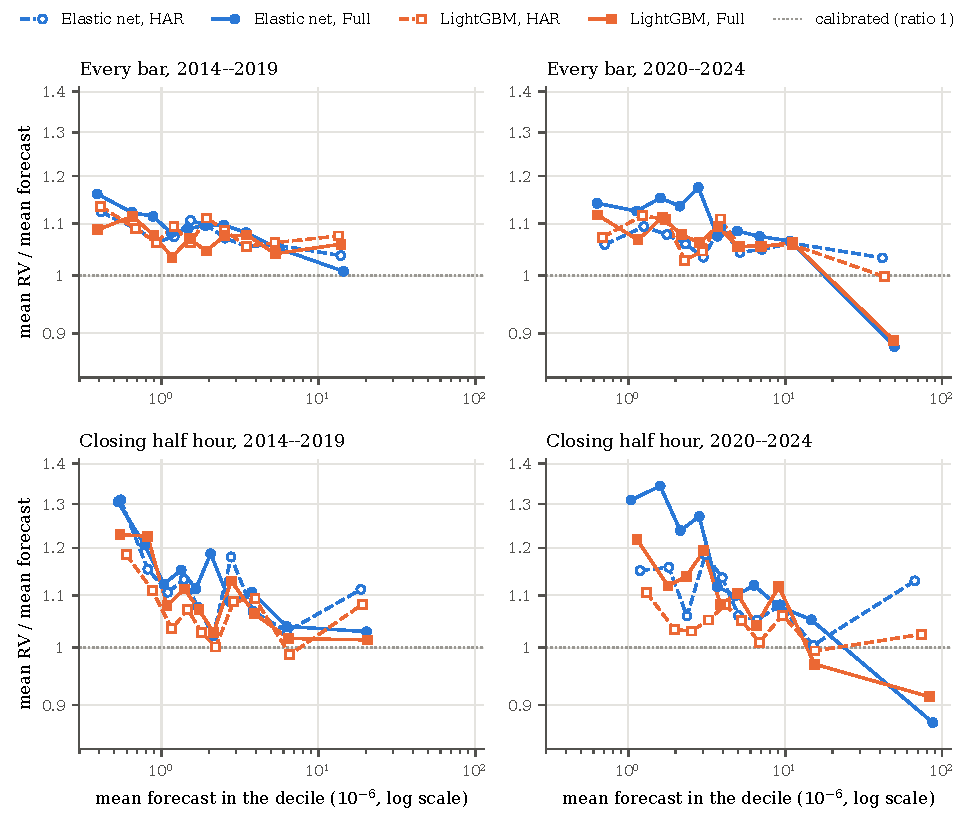
\includegraphics[width=\linewidth]{generated/rehaul_calibration.pdf}
\caption{Calibration by forecast decile. Within each decile of the forecast, the mean realized variance relative to the mean forecast (vertical axis; 1: calibrated, above 1: the forecasts are too low), plotted at the decile's mean forecast (horizontal axis), for the elastic net and LightGBM on the HAR benchmark (open markers, dashed) and on the full predictor set (filled markers, solid); log scales. Top: every bar of Table~\ref{tab:rh_oos}; bottom: the 16:00 bar (the forecast of the closing half hour). Left: \rhcaYearsPre{} ($\rhcaNdaysPre$ days); right: \rhcaYearsOos{} ($\mathcal T_{\mathrm{close}}$, $\rhcaNdaysOos$ days). On every bar in \rhcaYearsOos, the ratio of the full-set elastic net falls from \rhcaBotDecRatioEnetFullBarOos{} in the bottom decile to \rhcaTopDecRatioEnetFullBarOos{} in the top decile (HAR benchmark: \rhcaBotDecRatioEnetHarBarOos{} and \rhcaTopDecRatioEnetHarBarOos), and the top decile carries \rhcaTopDecSeEnetFullBarOos\% of its squared error.}
\label{fig:rh_calibration}
\end{figure}
